\chapter*{}

\vspace*{\fill}

\begin{flushright}
\begin{adjustwidth}{2.0cm}{}
\raggedleft\scriptsize\emph{A \versal{\emph{Coleção Ataque}} irrompe sob efeito de junho de 2013.
Esse acontecimento recente da história das lutas sociais no Brasil, a um só
tempo, ecoa combates passados e lança novas dimensões para os
enfrentamentos presentes. O critério zero da coleção é o choque com os
poderes ocorrido durante as \emph{jornadas de
junho}, mas não só. Busca"-se captar ao menos uma pequena parte do fluxo de
radicalidade (anti)política que escorre pelo planeta a despeito da
tristeza cívica ordenada no discurso da esquerda institucionalizada. Um
contrafluxo ao que se convencionou chamar de onda conservadora. Os
textos reunidos são, nesse sentido,
anárquicos, mas não apenas de autores e temas ligados aos
anarquismos. Versam sobre batalhas de
rua, grupos de enfrentamento das forças policiais, demolição da forma"-prisão que
ultrapassa os limites da prisão"-prédio. Trazem também análises sobre os
modos de controle social e sobre o terror do racismo de Estado. Enfim, temas de enfrentamento com
escritas que possuem um alvo.}

\emph{O nome da coleção foi tomado de um antigo
selo punk de São Paulo que, em 1985, lançou a coletânea \emph{Ataque
Sonoro}. Na capa do disco dois mísseis, um soviético e outro
estadunidense, apontam para a cidade de São Paulo, uma metrópole do que
ainda se chamava de terceiro mundo. Um anúncio, feito ao estilo audaz
dos punks, do que estava em jogo: as forças rivais atuam juntas contra o
que não é governado por uma delas. Se a configuração mudou de lá para
cá, a lógica e os alvos seguem os mesmos. Diante das mediações e
identidades políticas, os textos desta coleção optam pela tática do
ataque frontal, conjurando as falsas dicotomias que organizam a
estratégia da ordem. Livros curtos para serem levados no bolso, na
mochila ou na bolsa, como pedras ou coquetéis molotov.
Pensamento"-tática que anima o enfrentamento colado à urgência do
presente. Ao serem lançados, não se espera desses livros mais do que
efeitos de antipoder, como a beleza de exibições pirotécnicas. Não há
ordem, programa, receita ou estratégia a serem seguidos. Ao atacar
radicalmente a única esperança possível é que se perca o controle e,
como isso, dançar com o caos dentro de si. Que as leituras produzam
efeitos no seu corpo.}

\medskip

\textsc{acácio augusto \& renato rezende}
\end{adjustwidth}
\end{flushright}
\thispagestyle{empty}

\pagebreak

\vspace*{\fill}\thispagestyle{empty}
\begin{flushright}
\emph{Paratodos}
\end{flushright}
\pagebreak

\vspace*{\fill}\thispagestyle{empty}
\begin{flushright}
\emph{{[}\ldots{}{]} apenas discordamos disso com afeto.}
\end{flushright}

\chapter*{Apresentação}
\addcontentsline{toc}{chapter}{Apresentação, \emph{por Bruno Cava}}
\hedramarkboth{Apresentação}{}

\begin{flushright}
\textsc{bruno cava}\footnote[*]{Mestre em Filosofia e Teoria do Direito
(\versal{UERJ}) e professor de cursos livres. É autor de \emph{A multidão foi
ao deserto} (Annablume, 2013) e coautor de \emph{A terra treme: Leituras do
Brasil de 2013 a 2016} (Annablume, 2016) e \emph{A Constituição do Comum} (Revan,
2017). Organizou, com Murilo Duarte Costa Corrêa, \emph{Pensar a Netflix: Séries
de pop filosofia e política} (D’Plácido, 2018). Mantém, no Youtube, o
canal \emph{HorAzul}.}
\end{flushright}

Quando conheci o Murilo, mal pude acreditar que tinha diante
dos olhos o autor de tantos textos de ataque --- no sentido musical do
termo --- que eu admiro. Aquele corpo franzino, branquinho, com óculos de
aro circular e um visual meio ``Harry Potter'' (sobre o qual ele mesmo faz
troça) podia modular a escrita segundo um envelope bastante amplo de
intensidades. O mesmo autor que, em 18 de junho, no auge da
mobilização de 2013, escrevia em seu blog pessoal \emph{A navalha de
Dali} que ``A liberdade só deixa de ser um conceito abstrato na medida em
que se converte em revolta profunda e real''. O mesmo que, em meio a uma
campanha geral de descrédito e criminalização, conseguia enxergar o que
de singular há no fenômeno brasileiro dos black blocs. Enxergava e, por
meio da escrita, prolongava. Porque o black bloc, no levante da
multidão, tem sido antes um efeito multiplicador e transformador, mais do que
qualquer grupo orgânico, apaziguado numa identidade visual. O black bloc
é algo que acontece.

Meu interesse comum com o Murilo costuma ser o pós"-estruturalismo
francês: Michel Foucault, Gilles Deleuze, Félix Guattari e quejandos.
Mas não pense o potencial leitor, que agora cheira estas linhas, que tem
nas mãos um livro recheado de jargões e paralogismos anistóricos --- um
livro ``pós"-moderno'', na acepção ruim do termo, escrito para
\emph{hipsters} refugiados da rua em uma espécie de esnobismo cult. Não há nada
aqui que possa ser mais distante do relativismo, de valores flutuantes e
não"-referenciais, ou da morte do sujeito celebrada \emph{em si mesma} ---
sem casar o esforço da destruição com a alegria da criação. Murilo é um
leitor intensivo e rigoroso, mefistofélico, e cultiva o mau hábito de
atualizar ``teorias viajantes'' segundo manobras impensadas.

Neste, Foucault, Deleuze, Guattari etc. se encontram com Tom Zé,
Décio Pignatari, Caetano Veloso, Rita Lee, Gilberto Gil e, eminência
parda do livro, Oswald de Andrade. Murilo, com grande efeito, provoca
uma afinidade eletiva. Mas também é um livro em que o pós"-estruturalismo
francês viaja para reencontrar --- outra vez diferente! --- as barricadas
e o fogo político agenciador de investimentos libidinais, que os
``pós"-modernos'' esqueceram. Se a apreensão \emph{radical chic} da
``teoria francesa'', de extração norte"-americana, fez de tudo para
confiná"-la a galerias, libretos de vanguarda e o ``alto circuito'' das
artes, aqui, Murilo se deixa chinchar o pensamento pelos blacks blocs
para conferir à teoria a potência e o sentido políticos que o evento
reclama. Pois estética e estilo --- o dos black blocs é \emph{all over}
--- têm tudo a ver com política. Em chave etnográfica, comparece também
Pierre Clastres, ativado na medida em que o tema do livro é, sobretudo,
uma \emph{anticomunidade}: como as tribos quinhentistas das terras
baixas sul"-americanas, é uma em permanente processo de desfiliação e
conjuração do estado.

A crítica radical da metafísica da presença não vem substituída por um
retorno nostálgico à ``presença selvagem'', do corpo em carne e osso,
aqui e agora. Como se, diante da inapelável execução do sujeito, não nos
sobrasse outra alternativa senão voltar a sentir"-nos vivos pulando de
\emph{bungee jump}, se acabando em raves pós"-punks ou exercendo
deliberadamente o donjuanismo. Esses seriam tempos mortos, homogêneos,
cuja intensidade repete, indiferente, o mesmo ego girando ao redor da
falta. Seria a única alternativa em tempos de black blocs? A resposta de
Murilo é não. A desterritorialização do sujeito autocentrado e
autoportante da modernidade não significa, pois, que outros corpos
não possam ser recompostos --- politicamente, esteticamente --- no comum
das barricadas, na expressão constituinte, na arte violenta dos
encontros amorosos pela cidade. Este é um livro sobre o que os corpos
podem, corpos que nas ruas e redes desembotam e recuperam o viço. Diriam
Deleuze e Guattari, desterritorializar não funciona sem a
reterritorialização. ``Toda ação black bloc se define como a criação de
um entretempo onde a política se tornou possível.'' Fazer corpo político
é também constituir outra terra.

Murilo sabe muito bem, sim, fazer corpo --- um híbrido, um devir"-black
bloc, um Harry Potter subdesenvolvido das cavernas. Este livro
testemunha a sua vitalidade irreverente, ele próprio um importante
momento da recomposição político"-corporal que estamos vivendo.



\chapter*{Prefácio}
\addcontentsline{toc}{chapter}{Prefácio, \emph{por Peter Pál Pelbart}}
\hedramarkboth{Prefácio}{}

\begin{flushright}
\textsc{peter pál pelbart}\footnote[*]{Filósofo e ensaísta, é
Professor Titular do Departamento de Filosofia (\versal{PUC"-SP}).}
\end{flushright}

Prepare"-se o leitor. Não há neste livro"-manifesto uma única frase que
não seja pura irreverência, provocação, argúcia, arremesso teórico. Ao
abordar a atitude black bloc, o autor opera uma reversão
impiedosa: tira a máscara da democracia ocidental e de sua versão
brasileira. Sim, desta que invoca constantemente a paz social, embora se
assente na violência cotidiana do Estado, que garante a aberração
socioeconômica, jurídica, politiqueira e midiática.

Ao leitor é oferecida aqui uma chave que devolve sentido àquilo que
parecia vandalismo, baderna, anarquia, niilismo. Quando invoca a
cumplicidade entre a violência e o Estado, o rosto e a captura, o
contrato e a obediência, a mídia e a disciplina simbólica, aparece o
sentido da ação direta que visa, através do corpo, ``contestar
abertamente a repartição entre legalismos e ilegalismos''.

As táticas black bloc, portanto, são entendidas como uma
contraconduta física que dessacraliza o ordenamento jurídico, expõe a
violência do Estado, bem como as iniciativas de criminalização da
manifestação política: ``Toda revolta é, em primeiro lugar, a recusa
profunda, afetiva e vital da repartição do lícito e do ilícito. Por
isso, ela margeia estrategicamente o ilícito, vaga nos limiares
indecisos da lei''.

Mas nada aqui é austero --- há muito humor, etologia, música, poesia: a
defesa do \emph{bicho} contra a barbárie civilizada, do \emph{happening}
contra os códigos morais, bem como conexões inusitadas com o
tropicalismo e a estética concretista, Tom Zé, Caetano, Décio Pignatari
(``o Brasil está um cu''), filosofemas de procedências diversas
(``Amarildo, não o \emph{homo sacer}, é o corpo político paradigmático
da legalidade de democracia aparente do Brasil contemporâneo'').

O leitor pode concordar ou discordar, ficar irritado e até furioso com
este libelo, ou apreciá"-lo e se deliciar, mas não pode deixar de
reconhecer que Murilo Duarte Costa Corrêa, formado em Filosofia do
Direito, nos ajuda a entender um dos pontos mais cegos dos movimentos
iniciados em Junho nas cidades brasileiras.

A defesa radical de uma democratização do pensamento no Brasil também
passa por esta abertura --- a de acompanhar o esboço de um pensamento
black bloc, cujos frutos e efeitos ninguém tem como antecipar.

\part{\textsc{filosofia black bloc}}

\chapter{Manual de Junho}


Cinco anos depois, Junho de 2013 continua a ser o evento recente mais
enigmático e o mais pregnante para compreender os destinos da política
no Brasil contemporâneo. As ruas daqueles dias testemunharam o
transbordamento da matéria múltipla e em movimento de que o desejo
social é feito. Com seus perigos e chances, correntes de desejo e crença
afluíram nas noites das metrópoles; aos seus fluxos, seguiu"-se um grande
número de trabalhos que, sob o pretexto de analisar os elementos
conjunturais que favoreceram a emergência dos protestos, disputavam a
semântica do levante brasileiro (Ortellado 2017).

Isso instaurou um cenário analítico em que a aparente heterogeneidade
das leituras sobre Junho contrastava com a submissão do evento a toda
sorte de interpretações autocomplacentes que --- apesar da variedade ---
deixavam escapar a matéria efetivamente plural e em movimento de que
Junho foi feito. Escrevendo a fórceps, e premida pela urgência de
oferecer respostas diante da corrosão das velhas categorias, a crítica
política nacional perdeu a oportunidade de compreender Junho em meio a
leituras parciais do fenômeno e, ao mesmo tempo, carregadas de
pretensões de totalidade. De lá para cá, não cessamos de fazer funcionar
as nossas velhas armas teóricas como gastos leitos de Procusto.

Apesar de as interpretações autocomplacentes seguirem mutilando o
essencial, compreender Junho é o esforço coletivo para transcrever a
multiplicidade das forças sociais e políticas que emergiram durante
aqueles dias e noites: o levante foi um acontecimento do comum (Cava e
Mendes 2017: 21--23); foi a expressão de multiplicidades de linhas de
fuga que definem um campo social.

\section{O Estado contra o black bloc}

Quando a maior parte dos analistas
resolveu analisar Junho mais em termos de ato que de potência, mais em
termos de atualidade nua do que de diferença social e política, era
sinal de que os intelectuais cumpriam seu papel na divisão social do
trabalho: esgotar o acontecimento"-Junho, submetendo as multiplicidades
rizomórficas de desejo e de crença daqueles dias e noites ao molde
cômodo das grandes categorias segmentares e de Estado.\footnote{Eis o
  ponto em que ``o pensamento toma emprestado sua imagem
  propriamente filosófica do Estado como bela interioridade substancial
  ou subjetiva'' (Deleuze 1998: 21).} Seu efeito é o de bloquear
antecipadamente qualquer interpretação de Junho que não passe pelo
filtro das categorias ``maiores'' --- os binarismos que servem para fixar
e codificar as linhas de criatividade que definem um campo social em
função de referenciais preestabelecidos~---, forcluindo (Lacan 1966:
558) todo o resto: isto é, todas as constelações de fugas sociais e
políticas possíveis.

Com isso, tentavam liquidar a possibilidade de pensar Junho em seus
próprios termos, submetendo as multiplicidades do acontecimento à
avaliação homogênea de seus impactos na esfera tradicional da política.
Não cessamos de ler Junho sob o ponto de vista de Brasília, dos palácios
de governo, dos partidos recusados pelas multidões, da surpresa e da
inércia dos poderes constituídos, da decadência da representação formal,
das ficções democráticas fissuradas, das categorias de classe cerradas
para o social, das noções consumeristas de serviços públicos ou das
relações laxistas e abstratas travadas entre sociedade e Estado. Pensar
Junho nesses termos torna"-se então ``capturar e destruir'' sua potência
específica. Não é por acaso que boa parte das interpretações de
intelectuais se parece tanto com os discursos de políticos, policiais ou
jornalistas da grande imprensa que vimos circular naqueles dias (e.\,g.,
Chauí 2013; Souza 2015; Nogueira 2014; Rosenfeld 2014).

Não se trata de afirmar a existência de um bloco de leituras homogêneas.
Alguns intérpretes de Junho (e.\,g., Pinto Neto 2013; Cocco 2014; Arantes 2014;
Nunes 2014; Avelar, 2017; Cava e Mendes 2017) leram o
acontecimento em seu terreno imanente. No entanto, trata"-se de exceções
que confirmam a regra: a maior parte das análises dedicadas a Junho
preteriu o acontecimento em razão das explicações globais, das
categorias segmentares e das ciências maiores (Deleuze e Guattari 2007:
24--43). Sem serem afetados por Junho, continuaram a fazer do pensamento
uma dobra da forma"-Estado, e deram à luz um dos mais orgânicos e tesos
dispositivos de saber"-poder dos últimos decênios, neutralizando os
traços de uma emergência efetiva contida em Junho. No âmbito do
pensamento, esse intelectuais foram a encarnação do Estado contra Junho.

Suas análises aparentemente heterogêneas resultaram especialmente
similares com relação ao black bloc. Entre analistas representantes de
espectros políticos bastante distintos, é possível encontrar descrições
multifatoriais das razões que teriam levado aos protestos: a ``ausência
de correspondência entre carga tributária e serviços públicos''
(Figueiredo 2014: 63); a ``crise de valores enfrentada pela sociedade
brasileira'' (Rosenfeld 2014: 139); uma ``crise de longa duração''
atribuída à ``falta de dirigismo político dos governos do \versal{PT}'' (Nogueira
2013: 21--22); e a possibilidade de ``fazer demandas aos poderes
constituídos'' (Chauí 2013). É possível ouvir, sob essas
interpretações autocomplacentes, ecos que vão das ambições
capitalísticas nada subterrâneas da \versal{FIESP} à categoria de guerra de
posição de Antonio Gramsci.

Ney Figueiredo (2014: 63) destaca os significativos ``prejuízos
materiais do comércio e do sistema bancário'' com as depredações; Denis
Rosenfeld (2014: 139--143) qualifica o black bloc como ``grupos
que depredam e saqueiam, parecendo ser meros criminosos comuns quando,
na verdade, são agremiações políticas cujo propósito é levar o país a
uma crise institucional'', ``grupos de ideologia
anarquista/socialista/comunista, de espírito {[}\ldots{}{]} contrário à
economia de mercado, ao direito de propriedade, ao estado de direito'';
à esquerda, Marilena Chauí (2013) afirmou encontrar no black bloc
tendências ``mais fascistas do que anarquistas'', desqualificando"-os
como sujeitos revolucionários na medida em que não têm ``uma visão do
que é inaceitável no presente e qual a institucionalidade futura que se
pretende construir''; por fim, Marco Aurélio Nogueira (2013: 102--103),
além de reafirmar que o black bloc atua ``com táticas
fascistas'', afirma se tratar de ``minorias do mal'' que agem para
``humilhar as maiorias. {[}\ldots{}{]} Não querem confluir para nenhuma
maioria, porque acham que as maiorias são passivas e `dóceis'.
{[}\ldots{}{]} Usam máscaras porque precisam de identidade.
{[}\ldots{}{]} não são progressistas, nem muito menos radicais da
democracia''. Finalmente, ``o que sobra de suas ações é
péssimo para a democracia e a reforma social''.

Apesar de estarem politicamente distantes entre si, os textos citados
permitem perceber que os adeptos da tática black bloc foram qualificados
à direita e à esquerda como ameças violentas e ``fascistas'' à ordem
democrática liberal, e acusados de atuar de forma niilista e
antipolítica. Entre intelectuais de esquerda e de direita, os conteúdos
semânticos desses termos variam significativamente, mas é interessante
notar como o black bloc foi objeto de uma recusa visceral e em bloco por
intérpretes de praticamente todos os matizes políticos representados na
esfera formal. De onde viesse o discurso, uma coisa era certa: os black
blocs deveriam ser repudiados pela sociedade como um fenômeno
antissocial e reprimidos pelo Estado como criminosos políticos --- quando
não como criminosos comuns, uma vez que não exprimiam qualquer
reivindicação legítima.

Um outro filão da esquerda tradicional, que se encontra bem representada
pelo recente livro de Eugenio Bucci (2016), analisou as ações diretas da
tática black bloc sob o ponto de vista de sua relação com a performance,
criticando"-as por sua suposta solidariedade com os circuitos
capitalistas ativados na sociedade do espetáculo. A tese de Bucci produz
uma dupla neutralização: de um lado, Junho é apresentado como um
fenômeno mais cultural do que político, alienado à forma do espetáculo e
do desejo coletivo curvado à imagem (Bucci 2016: 118) --- como se o
espetáculo e a imagem não fossem em si mesmos políticos; de outro, na
era da produção industrial do imaginário e do entretenimento, quando
olhar e trabalhar se convertem em uma só e mesma coisa (Bucci 2016:
136), ``a estética dos protestos de rua {[}\ldots{}{]} passa pelo
capital'' (Bucci 2016: 125), e o black bloc é definido como um clichê,
um modelo de comportamento emergente que permite ao telespectador um
gozo escópico --- por atração ou repulsão --- e ao adepto da tática, um
mais"-de"-gozar no olhar do mundo (Bucci 2016: 134). Com efeito, seria de
se perguntar que tipo de ação política não se encontra, hoje, engastada
de algum modo nos circuitos do capital, do espetáculo ou do valor de
gozo, especialmente se as nossas sociedades passam a ser organizadas por
referenciais perversos (Melman 2003: 51--52). Haverá, para a ação
política, um ``fora'' da perversão do espetáculo ou do ecumenismo do
capital? Ou não encontramos perversão também precisamente no olhar de
quem, gozando, delata o gozo no olhar ou o mais"-de"-gozar no ato político
alheio?

Essas obras conservam também um paralelismo formal notável. Nelas, o
black bloc aparece como um fenômeno lateral, minoritário e secundário
relacionado a Junho, do qual parece ser necessário desembaraçar a
análise o mais rápido possível para se poder chegar ao seu núcleo
efetivamente político. A forma pela qual isso geralmente se processa
consiste em descrever suas ações de maneira aparentemente imparcial,
deduzir sua apoliticidade, discutir seu caráter violento, concluir pela
sua incompatibilidade com a democracia e desconectá"-las das
manifestações majoritárias, politizadas e pacíficas. Descartando suas
expressões supostamente antipolíticas e selvagens, os analistas podem
dedicar"-se a descrever um Junho domesticado. A última fronteira em que o
Estado combate o black bloc é ao domesticar o pensamento de Junho, ao
submeter o evento a uma intelectualidade de Estado.

\section{Pensar o black bloc}

Nesses termos, o black bloc é tratado
analiticamente como um subconjunto sem relação com as demandas do campo
social; é literalmente anulado como sujeito político. Talvez por isso
seja relativamente raro encontrar nas obras sobre Junho capítulos
dedicados a analisar o black bloc, ou mesmo livros. Geralmente, a
análise se liga à necessidade de discutir a legitimidade política do uso
da violência nos protestos. Isso é sintomático porque, ao mesmo tempo em
que muitos desses intérpretes não cessam de tentar varrer o fenômeno
para debaixo do tapete analítico, o black bloc parece se acumular,
escapar e retornar a todo instante, não raro como o elemento violento
que permitiria determinar a novidade específica de Junho (Gohn 2014:
76), ou como o elemento que permitiria distinguir claramente entre
manifestantes politizados e vândalos programaticamente niilistas
(Nogueira 2013: 102--103). Com efeito, o truísmo de que as ações diretas
são intrinsecamente violentas é constantemente reafirmado, embora o
conceito de violência seja sempre um pressuposto não"-analisado\footnote{Um
  exemplar pode ser encontrado no texto de Maria da Glória Gohn (2014:
  76--77), em um trecho que se dispõe a definir violência, mas não
  consegue oferecer qualquer conceito claro e determinado para o
  contexto da violência imputada automaticamente às ações diretas: ``Há
  várias interpretações na literatura contemporânea sobre a violência.
  Seu significado é amplo e contraditório, depende do ponto de vista do
  autor do discurso. Pode aparecer como resultado de tensões e conflitos
  nos atos de cidadania insurgente, tendo por base um repertório
  universalista de direitos {[}\ldots{}{]}; ou como fruto de contextos
  situacional e relacional {[}\ldots{}{]}. Em qualquer vertente, ela
  surge como algo construído a partir da ação de indivíduos nas suas
  relações sociais e nos contextos sociopolíticos e culturais que
  vivenciam, atribuindo significados a seus atos e discursos
  {[}\ldots{}{]}. Atos de violência contra o patrimônio público e privado
  ocorreram em junho de 2013 {[}\ldots{}{]}''. Para uma discussão mais
  informada e contextualizada do conceito de violência, cf. Francis
  Dupuis"-Déri (2014: 79--118).}.

De outro lado, é preciso registrar a menos ruidosa publicação de textos
como ``Black Blocs'' (Dupuis"-Déri 2014) e ``Mascarados'' (Solano et al.
2014), que contribuíram para colocar em perspectiva a política do black
bloc suspendendo a disputa sobre a semântica de Junho. Enquanto
Dupuis"-Déri oferece uma pesquisa densa e informativa sobre a genealogia
da tática no cenário global, Esther Solano produz uma pesquisa de campo
com os adeptos da tática em São Paulo. ``Black blocs'' descreve o
fenômeno a partir de seus traços históricos, estéticos, políticos e
táticos mais globais, e ``Mascarados'' traça um perfil social,
existencial e político das pessoas que se encontram por trás das
máscaras: jovens de classe média"-baixa, usuários dos serviços públicos,
trabalhadores precários, relativamente politizados, que confrontam de
maneira violenta --- e, às vezes, reprovável --- a violência sistêmica e a
precariedade do Estado brasileiro (Solano et al. 2014: 17--43).

A corajosa beleza da pesquisa de Esther está no fato de que a etnografia
faz falar as vozes silenciadas, perguntando ``quem são?'', ``quais as
causas do enfrentamento?'', ``qual a mensagem por trás das máscaras e
das ações diretas?'', ``o que entendem por violência?'' etc. Essa
operação sensível faz perceber que, sob as máscaras, há pessoas e
sonhos, insiste uma cultura política viva sob um conjunto de
comportamentos aparentemente estereotipados ou espetaculares. No
entanto, eis o limite interior à pesquisa etnográfica: ela pode revelar
as pessoas sob as máscaras, as suas relações com o heterogêneo
(indivíduos, grupos, instituições etc.), induzindo certos traços
holísticos; mas tende, sempre, à definição de um grupo.

Se quisermos levar Junho a sério, é preciso levar o black bloc a sério e
produzir um modo do pensamento que corresponda ao fenômeno. Não
perguntar ``o que é o black bloc?'', mas como o black bloc nos violenta
a pensar --- já que pensar é a menos inata das atividades (Deleuze 2006: 214). Produzir, no pensamento, o devir"-black bloc da filosofia; criar
uma filosofia black bloc. Talvez não baste escutar as vozes silenciadas
e dar voz a elas; é preciso perguntar, também, de que outras forças, de
que outros gritos e de que outros mundos possíveis essas vozes são a
expressão? Que povo por vir elas prenunciam? Para tanto, é preciso
conjugar as superfícies pessoais e as identificações de grupo, expressas
nos achados etnográficos, com a descrição micropolítica das linhas de
fuga e de ruptura que definem um campo social.

Jamais estivemos verdadeiramente à altura de enfrentar o problema que o
black bloc nos propõe em toda a sua extensão. Isso requer que
suspendamos por um momento o juízo moral e as questões contumazes: ``o
que é o black bloc?'', ``quem são os adeptos da tática?'', ``são
justificáveis, violentas ou lícitas as ações diretas?'', ``como lidar
com alguns efeitos trágicos?''. É urgente mergulhar na profunda
antiontologia que o black bloc encarna. Aposentemos a ideia do black
bloc como um subconjunto social de Junho de 2013, passível de
identificar"-se com um grupo de jovens subproletários, relativamente
politizados, usuários de transportes públicos, para fazer o black bloc
funcionar como um analisador geral do tipo de vetor sociopolítico que
esteve em jogo nos levantes. Para tanto, não basta tornar visível o
ponto de vista por trás das máscaras, é preciso tornar as máscaras
mesmas um ponto de vista e, através dele, fazê"-las falar: eis o que
converte a etnografia em uma potente antropologia política, capaz de
demarcar as linhas gerais de ataque que o black bloc distendeu --- não
como grupo, nem como tática, mas na dupla condição de singularidade
política daqueles dias de Junho e de força capaz de afetar o pensamento.

\begin{center}
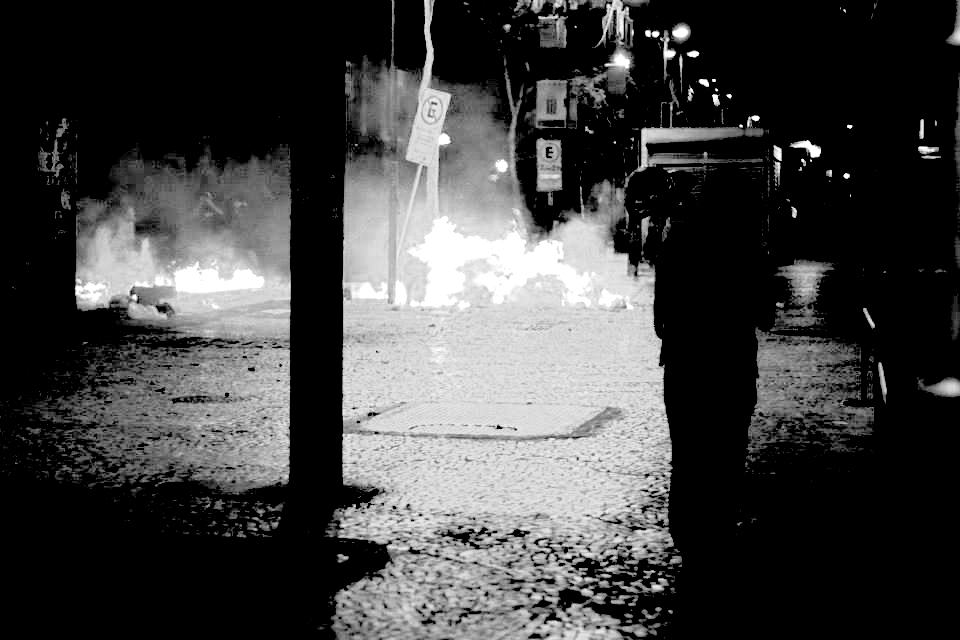
\includegraphics[width=9cm,height=6.1cm]{Imgs/img2.jpg}
\emph{Niilismo}, 2013
\end{center}

\section{Agenciamentos}

A única violência cometida pelo black bloc foi
nos levar a pensar. Foi impedir que permanecêssemos estúpidos no seio de
uma possibilidade unicamente abstrata do pensamento. Nem vitrines, nem
caixas eletrônicos, nem câmeras de vigilância destruídas ou carros da
polícia tombados ou incendiados. Nada disso é violência. Seu único
vandalismo é precisamente este: açoitar todos os inatismos, violentar a
um modo de pensar a contrapelo dos tribunais \emph{ad hoc} do juízo.

Um black bloc arremessa contra o que o real tem de insuportável uma
outra forma de vida e de sensibilidade à qual é impossível permanecer
indiferente. Gênese de afetos, produção de diferença a partir da
indiferença. Não é por outra razão que seus críticos logo ameaçaram os
intelectuais que assumiram posturas públicas de compreensão e análise de
suas ações diretas e os acusaram de serem cúmplices ou responsáveis.
Pensar em conexão corpórea com aquilo que nos \emph{força }a pensar
tornou"-se um crime. A culpa é \emph{a priori, }indubitável. E eles têm
razão. Pensar a fenomenologia da revolta como corpo encarnado de uma
ontologia da liberdade equivale a captar no ar uma \emph{filosofia black
bloc}: instaurar uma apologia proliferante. Nas suas margens, emerge
tudo aquilo que se tornou insuportável em uma democracia de tradição
autoritária e em um Estado de Direito em que a exceção foi transformada
em regra para manter a seletividade funcional dos aparelhos de controle
criminal e judiciário.

Nossos corpos torturados todos os dias por condições de trabalho e de
vida inumanas, ou nos transportes coletivos, nossas vozes sufocadas
pelos cartéis da liberdade de expressão, não aguentam mais. Eis os mil
índices sutilizados de que jamais deixamos de ser aquilo que fomos para
as ditaduras: corpos que não aguentam mais. Eis a condição material que
permite entrever, porque a adianta, a reversão da primazia aristotélica
do ato sobre a potência --- tudo o que interessa para pensar são as
potências dos corpos~---, da primazia hobbesiana do instituído sobre o
constituinte e da superioridade cartesiana do \emph{cogito }sobre o
corpo. Tudo se afirma de uma só vez na multidão contra o Um, se por
multidão compreendermos multiplicidades de multiplicidades de corpos.
Singularidades irredutíveis, os corpos jamais são ativados ao mesmo
tempo ou afetados da mesma maneira. Todos eles se movem, porém, na
univocidade de um desejo de multiplicar o múltiplo.

Agenciados entre si, seus afetos são como armas, propulsões, impulsos e
projéteis capazes de rearticular todas as dimensões do tempo;
testemunham uma vida inorgânica que atravessa a totalidade movente do
real. Fim da Polícia Militar, democracia real, crise de representação,
tarifa zero, passe livre, serviços públicos padrão \versal{FIFA}, fim da cultura
da impunidade, efetividade e ampliação dos direitos humanos, liberação
animal --- os corpos querem mais. Os corpos querem tudo e não têm modos:
constituem os seus por invenção. Precipitam, no presente, algo que é da
ordem de uma memória para o porvir. Eis o que torna a tarefa de uma
\emph{filosofia black bloc} uma espécie de classicismo metafísico:
subtrair as imagens da revolta da forma política negativa a que foram
lançadas pela opinião comum. \emph{Sophía} contra a \emph{doxa.}
Trata"-se ainda do gesto nietzschiano que, no fim da Genealogia da Moral,
perscrutava, no seio aparentemente negativo do niilismo ascético, a
positividade imanente do desejo: ``Querer o Nada é ainda querer''.

\chapter{Panis et circencis}

\begin{center}
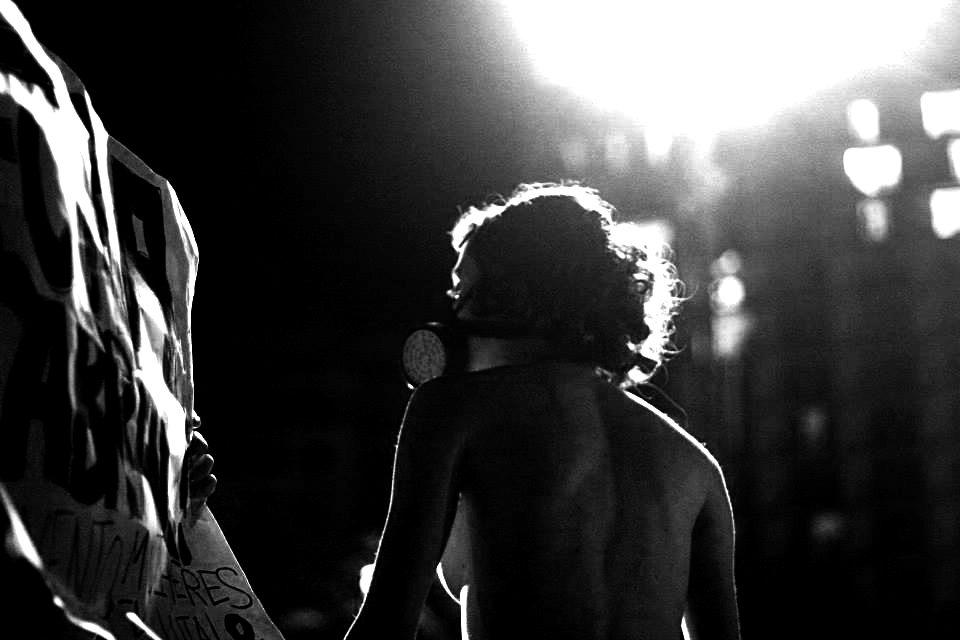
\includegraphics[width=9cm,height=6.1cm]{Imgs/img3.jpg}
\emph{3,20? Só vendendo meu corpo}, 2013
\end{center}

\section{Tudo começou com o corpo}

\subsection{Maus modos}

Ouve"-se o barulho dos talheres e pratos e a
conversa à mesa. Bocas cheias mastigam. Convém prestar atenção à
televisão. O rosto de um homem familiar, que veste uma voz grave e tem
uma gravata, conta histórias das ruas. Parece que puseram fogo em um
carro da televisão. Quebraram vidraças da prefeitura. Depredaram caixas
eletrônicos. Saquearam as Lojas Americanas. Um orelhão queimou. Atiraram
pedras. Construíram uma barricada. Bateram em um Coronel. Fugiram.
Picharam a estação do metrô. Tudo começou pacífico, mas terminou\ldots{}
terminou em vandalismo. É preciso dizer. É preciso usar as palavras
corretas. Essa gente não tem ideais. São baderneiros, vândalos,
bandidos, mascarados, bugios raivosos! Cobrem os rostos, os covardes.
Deveriam estar presos! Direitos Humanos para humanos direitos! E os
direitos humanos de quem tem de trafegar na Avenida Paulista? Pegar os
filhos pequenos na escola? Os direitos humanos de quem deixou o carro
parado na Avenida Brasil? Olha lá, começou a novela! Eu acho que o
direito de cada um termina onde começa o do outro. Não pode parar a
cidade inteira só para reivindicar\ldots{} reivindicar o quê, mesmo? Ora,
pensa bem: com o preço da passagem deve dar pra comprar um carro, um
carrinho 1.0 que seja. \versal{IPI} zero, juros baixos, duas mil parcelas. Você
paga e nem sente. Por que esses filhos da puta não compram logo um
carro? Um carro popular? Aí vão ver quanto é bom pagar \versal{IPVA}! Onde já se
viu?, ficar andando de ônibus. Tem é que morar mais perto, morar no
centro, perto do trabalho. Como não se dão conta? É que não têm
trabalho. Quer dizer, trabalho até tem, mas para quem quer trabalhar,
né? Não gostam. São uns moleques\ldots{}, ou bandidos. Mascarados de merda.
Tem que matar esses filhos da puta. A \versal{PM} tem que matar, não é possível.
Isso não é gente. Ouvi dizer que recebem Bolsa"-Família. Sim, sim, a
guerrilha que financia. Ouvi dizer que com o dinheiro do mensalão. A
cidade virou um campo de guerra. Isso que dá, votar num bando de
guerrilheiros. Eu não votei. É bolsa"-vagabundo. E um dia desses ainda vi
um deles pulando a catraca. Claro: não pagam, a passagem aumenta! São
uns vagabundos. Não são gente. A gente que é correto, paga imposto pra
tudo, até pra respirar, trabalha. A gente não tem direito nenhum. Esses
não são gente. Adoram uma baderna. Cem mil baderneiros na rua quebrando
tudo. Por que não quebram a própria casa, hein? Queria saber. Quero mais
é que a polícia mate todos eles. Arruaceiros. Baderneiros. Desgraçados.
Por isso (bufa, afrouxa o colarinho) me atrasei para chegar em casa. Só
sei que eu não aguento mais sustentar vagabundo. Não estão preocupados
com nada, esses filhos da puta. Animais. Viver ou morrer. Não importa.
Não importa.

\subsection{As pessoas na sala de jantar}

``O que conta aqui é
justamente o descontrole, o processo claro de inversão, de avessamento,
de começar o jantar pelo meio, de dispensar as cerimônias de nascer e
morrer e errar o rumo dado, o que, no caso, é viver, o gesto livre e
propenso ao erro, que costuma acontecer entre o nascimento e a morte''
(Jaffe 2010: 34). O desejo de libertação contra o ritual da sala de
jantar. Eis os termos de uma tensão que Celso Favaretto (2007: 102)
identificava no coração de \emph{Panis et Circencis} --- a canção"-força,
de Caetano Veloso, gravada pela banda Os Mutantes no \versal{LP}
\emph{Tropicália}, e que era, também, seu subtítulo incidental. De
alguma maneira, a tensão entre libertação e ritual, desejo e sala de
jantar, anunciaria nos termos simbólicos dessa canção de Caetano uma
espécie de triunfo de antevéspera da ordem cotidiana contra \emph{uma
outra} ordem onírica, ou inconsciente, que o surrealismo tropicalista
distendia. Toda a liberação e todo desejo parecem conjugar"-se na forma
passada e esconder"-se sob a subjetividade cada vez mais dissolvida de um
``eu'' cuja verdade lírica é ser unicamente um ``ele'', terceira pessoa
indefinida. Forma quase"-impessoal do \emph{se} agenciada com uma
dimensão dissolvente do passado, que é também o inconsciente e o sonho.
``Eu quis cantar'', ``Mandei fazer'', ``Mandei plantar''. Passado,
inconsciente e imagens de sonho, móveis e colorantes, se organizam em
nome de um porvir bloqueado. Era 1968. Era maio na Europa, mas, no
Brasil, era dezembro. O governo militar decretava a suspensão de uma
série de direitos e garantias fundamentais previstos na Constituição de
1967. Os aparatos policiais e judiciários funcionavam a todo vapor.
Inventou"-se a polícia militar. Os efetivos aquartelados saíram às ruas.
Antes que o Brasil pudesse inventar seu próprio maio, em seus próprios
termos, dezembro se antecipara. O verão bloqueava a eterna primavera
autenticada. Triunfavam os afetos da ordem contra toda outra ordem de
afetos que, até hoje, jamais cessaram de pulsar nos corpos. Assim como
\emph{Panis et Circencis} é a montagem e desmontagem de um imenso
desfile de sonho interrompido pelos ruídos de uma conversa banal à mesa,
e pelo tédio profundo da valsa vienense que a rodeia, 1968 permanece, em
seu duplo sentido, um procedimento interrompido. 2013 teria sido o ano
intempestivo em que a invenção de nosso próprio maio de 68 viria
contestar a clandestina repetição daqueles velhos dezembros. O black
bloc atestava sua emergência. Nova encruzilhada em que o passado, o
inconsciente e as imagens de sonho inventariam um novo e singular
agenciamento. Entre as ocupações de nascer e morrer, cometer o maior dos
erros: a própria vida. Seja como for, tudo começou com o corpo.

\asterisc

Depois de muitos decênios de mudez e autismo político, de pactos
hipnóticos e de compromissos vergonhosos, experimentamos, como uma
lufada de ar novo, a emergência de eventos políticos de grande escala no
Brasil. As multidões que invadiram as ruas das principais cidades do
país não apenas fizeram de seus movimentos autônomos um espetáculo de
reapropriação do espaço público; mais profundamente, as multidões
reinventaram e ressignificaram este conceito que até então parecia
bloqueado, ou definitivamente deposto pela violência performativa dos
consensos eleitorais. As multidões das ruas deflagraram o que parece ser
o mais significativo processo de acumulação primitiva de democracia
desde a instauração dos programas de distribuição de renda dos governos
Lula (2002--2010) --- que, alguns anos mais tarde, mostrariam seu
viés desenvolvimentista e autoritário --- e, também, desde os movimentos
pela redemocratização e pelo exercício do voto direto no Brasil, um
pouco mais recuados. Os movimentos das redes e das ruas multiplicam em
seus próprios corpos a capacidade de reabrir os horizontes do espaço
público, de reinstaurar um potencial de invenção política de nossas
formas de vida que parecia definitivamente alienado na forma de nossas
instituições pretensamente democráticas e reconciliadas.

O encontro entre corpos de manifestantes e corpos policiais revela o
sentido prático, e a apropriação politicamente útil, que nosso
característico liberalismo autoritário tem feito do conceito vago de
``Estado Democrático de Direito''. Só se pode aferir a qualidade
democrática das instituições quando com elas se confronta a figura de
carne e osso, mas sem espessura, daquele que não tem direitos --- os
Amarildos que, virtualmente, somos cada um de nós frente às práticas
ilegais do Estado e de sua burocracia empresarial~---, ou quando essas
instituições impotentes reprimem violentamente as expressões
genuinamente democráticas que vêm das multidões heterogêneas das ruas.

As sociedades policiais forjam seus consensos e contratos inoculando o
medo e a impotência para agir. Aprendemos o medo quando assimilamos que
o direito é uma disciplina normativa coercitiva, violenta --- mas, na
defesa histérica do instituído, comumente corroboramos essa violência
real que os Estados e suas polícias praticam para conservar o direito na
finalidade mítica da segurança, da pacificação e em um conceito estéril
de democracia --- porque limitado à forma jurídica historicamente
decantada do já instituído. Aprendemos a impotência e a servidão quando
nos convencemos de que a violência política --- potência específica que
percorre nossos corpos individuais --- deve ser alienada à forma"-Estado,
único ente supostamente capaz de produzir um acordo de todos com todos.

As multidões das ruas são a prova de que tudo isso, porém, não passa de
mistificação contratualista, pacto hipnótico, alienação da potência
comum na forma do Um. É por isso que o Estado e os poderes constituídos
(o Um) as criminalizam sem cessar. É também a isso que se deve todo o
esforço semiótico dos oligopólios midiáticos e das oligarquias
intelectuais (à direita e à esquerda) para criar a cisão artificial
entre o manifestante pacífico e o vândalo, violento e antidemocrático,
que passa, cada vez mais, a ser considerado um criminoso \emph{a priori}
em virtude de pequenas ações que não constituem crime: vestir"-se de
preto, dissimular o rosto, usar máscaras, sentar"-se em uma escadaria,
formar um bloco, compor a linha de frente das manifestações, registrar
(em celulares, câmeras fotográficas ou de vídeo) atos de depredação e de
violência policial, ``portar'' substâncias comuns lícitas (como vinagre
ou desinfetante, e.\,g.) etc.

Somos perversamente habituados a enxergar as vitrines de bancos ou os
caixas eletrônicos como exemplares do direito democraticamente garantido
de propriedade privada; porém, estamos sintomaticamente desacostumados a
fazer o mesmo quando a propriedade coincide com as moradias miseráveis
dos pobres nas ocupações, nos morros e favelas. Somos perversamente
habituados a aceitar que agências bancárias tenham o direito de instalar
ofendículas em calçadas públicas para impedir que mendigos durmam sob
suas marquises à noite e importunem funcionários e clientes logo pela
manhã. Nesse caso, porém, acreditamos que tudo siga a ordem natural das
coisas: nenhum de nós ousa colocar em questão por que os bancos odeiam
tanto os indigentes que sua própria taxa de juros fabrica sem cessar.

O Estado, a polícia e as mídias nos bombardeiam com imagens de
depredação e vandalismo. O uso da semiótica do poder, dos termos
``vândalo'', ``mascarado'', ``baderneiro'', só não é maior que o
\emph{bodycounting} policial, que os altos índices de letalidade das
ações policiais que sempre aconteceram nas periferias e, há poucos
meses, com os protestos populares recentes, tornaram"-se visíveis também
nos centros das grandes cidades.\footnote{Segundo dados
  da Anistia Internacional, publicados em 27 de março de 2012, as
  Polícias Militares do Rio de Janeiro e de São Paulo mataram mais
  pessoas em 2011 do que o total de executados por vinte países que
  possuem a pena capital instituída. Somados, os índices de letalidade
  das atuações das \versal{PM}s do Rio e de São Paulo chegavam, só em 2011, à
  monstruosa cifra de 971 mortos, segundo o informe da Anistia
  Internacional; enquanto isso, os executados pela via da pena de morte
  em vinte países, somados, chegavam ao número de 670 no mesmo período.
  Já no informe 2016/2017 sobre o estado dos Direitos Humanos no mundo,
  a Anistia Internacional registra cifras ainda mais preocupantes. Entre
  janeiro e novembro de 2016, apenas no Estado do Rio de Janeiro, 811
  pessoas foram mortas pela polícia. Esses números assustadores
  significam que as execuções extrajudiciais representam, no Brasil, a
  instituição paralegal da pena de morte, e têm por alvo privilegiado,
  segundo dados da Anistia Internacional, vítimas jovens, negras, do
  sexo masculino, residentes nas periferias das grandes metrópoles do
  país.}

Quando jovens mascarados e sem rosto surgem nas ruas para contestar essa
ordem de coisas, é mais do que natural que sejam considerados
criminosos. Todavia, o black bloc nada mais é --- como os professores em
greve do Rio atestaram --- que o guarda"-costas da multidão contra o Um, a
linha de frente que impede que a violência policial tome maiores
proporções, atinja os manifestantes ``pacíficos'', e também reage com
certa violência, simbólica e dirigida a coisas, à intensificação da
violência policial.

A estratégia de criminalização do black bloc não é apenas simbólica, mas
jurídica. Sem qualquer fundamento plausível, na noite do dia 07 de
outubro de 2013, delegados de São Paulo autuaram um casal de
manifestantes com base na Lei de Segurança Nacional (Lei nº 7.170/83),
uma lei de conteúdo ditatorial, antidemocrática, progênita do Ato
Institucional nº 05, e que mesmo sob nosso pretenso regime democrático
não foi, ainda, explicitamente revogada. Como a estratégia falhou,
passaram aplicar ao black bloc a recente Lei 12.850, que define
organização criminosa,\footnote{Lei Federal nº
  12.850/2013, Art. 1º, § 1º. ``Considera"-se organização criminosa a
  associação de 4 (quatro) ou mais pessoas estruturalmente ordenada e
  caracterizada pela divisão de tarefas, ainda que informalmente, com
  objetivo de obter, direta ou indiretamente, vantagem de qualquer
  natureza, mediante a prática de infrações penais cujas penas máximas
  sejam superiores a 4 (quatro) anos, ou que sejam de caráter
  transnacional.''} sendo que nada, na forma de ação política black
bloc, corresponde ao tipo objetivo (``estrutura ordenada'',
``caracterizada pela divisão de tarefas, formal ou informalmente'') ou
ao tipo subjetivo (``com objetivo de obter, direta ou indiretamente,
vantagem de qualquer natureza'') da norma penal. Mesmo com certa demora,
a tentativa de tipificação --- mais política que jurídica --- foi,
inclusive, rechaçada pela Ordem dos Advogados do Brasil.

Não sendo bastante a covardia de criminalizar jovens que jamais tiveram
sequer direito a voz nessa democracia seletiva, pela primeira vez, desde
os anos de chumbo, temos presos políticos no Brasil e arriscamos ter
presos por crime de opinião. O delegado da Delegacia de Repressão a
Crimes de Informática (\versal{DRCI}) do Estado do Rio de Janeiro, Gilson
Perdigão, veio a público afirmar que ``quem publica comentários ou fotos
de apoio aos atos de vandalismo está cometendo
crime''.\footnote{``Apologia de atos de violência nas redes sociais pode ser considerada
  crime''. \emph{O Globo}, 15/10/2013.}
Supostamente, aqueles que se manifestam publicamente em defesa do black
bloc incorreriam no tipo de ``Incitação à prática de crime'', previsto
no artigo 286 do Código Penal.

Ingressamos em uma esfera perigosa, do controle da expressão e da
opinião política. O que está por trás da criminalização da mera opinião
em redes sociais é, em primeiro plano, a tentativa de minar o principal
lastro comunicacional e o meio organizativo dos manifestantes. Em
segundo lugar, produzir certa disseminação social do medo, pois o menor
gesto pode conduzir"-nos à prisão. Finalmente, talvez, o medo que os
poderes constituídos têm da simpatia que, malgrado todo o insistente
bombardeio semiótico dos oligopólios midiáticos, o black bloc desperta.
Um célebre apresentador de programas policiais fazia, em junho, uma
enquete ao vivo em rede nacional com o tema ``Você é a favor de protesto
com baderna? Sim ou não?''. É impossível esquecer o mal"-estar coletivo
do grupo de comunicação (que, talvez não por acaso, homenageia em seu
patronímico um grupo de genocidas coloniais) pela surpreendente resposta
da maioria. ``Sim, sou a favor de protesto com
baderna''.\footnote{Cf., sobre o episódio, o irônico
  ``Será que formulamos mal a pergunta?'', de Silvia Viana (\emph{In:}
  Maricato et al. 2013: 53--58).}

Mais um signo de que o terror governamental é autorreferente parece ser
o editorial publicado em 10 de outubro de 2013 na Gazeta do Povo,
intitulado ``cúmplices do vandalismo''.\footnote{``Cúmplices do vandalismo''. \emph{Gazeta
  do Povo}, Editorial, 09/10/2013.}
No texto, o editorial apócrifo afirma que ``Tão preocupante quanto a
violência dos black blocs é a construção, nas universidades, de um
arcabouço teórico que justifica a depredação verificada em grandes
cidades brasileiras''. Eis o triplo sintoma: em primeiro lugar, sintoma
daquilo que os poderes instituídos temem; em segundo lugar, sintoma
daquilo que deveria ser a função institucional das universidades ---
educar para o conformismo tecnicizante, o que as peças publicitárias das
universidades chamam eufemisticamente de ``desenvolver habilidades e
competências para inserção no mercado de trabalho''; em terceiro lugar,
o editorial forja um sintoma revelador da estratégia de poder dos
oligopólios da informação. Ignorando o princípio constitucional da
liberdade de cátedra, criminalizam, nas entrelinhas, o exercício do
pensamento ao mesmo tempo em que defendem a liberdade de informação e de
opinião apenas dentro dos códigos que seus editoriais estipulam.
Qualquer um que pense qualquer coisa fora dessa métrica, para além das
margens da crítica social autorizada pela imprensa, transforma"-se em
vândalo ou cúmplice --- e tudo se reduz à figura paradoxal do criminoso,
símbolo daquele que, porque já detém todos os direitos que as ``pessoas
de bem'' pretensamente não teriam, merece que nenhum deles seja
respeitado. Seja como for, qualquer pensamento desviante do pensamento
para o mercado e para o capital é considerado patológico ou criminoso.
Qualquer forma de filosofia não"-contratualista, que se exerça fora das
margens críticas controladas pelos titulares do aparato expressivo
oficial, se torna uma espécie de filosofia black bloc, filosofia
vândala da \emph{doxa }chancelada pelos valores sociais vigentes e
neutralizada nas escolas e universidades.

Fomos condicionados a pensar nos termos que convêm a essa repartição
histórica do poder: ``se está mascarado no espaço público é porque deve
alguma coisa, vai aprontar alguma, tem algo a esconder''. É urgente
desaprendê"-lo. Jamais nos damos o direito de perguntar, por exemplo,
``qual a qualidade democrática de instituições que não permitem a toda
uma geração de jovens o exercício da liberdade fundamental,
constitucionalmente assegurada, de manifestação, a não ser que
dissimulem seus rostos?''. O black bloc --- grupamento de autodefesa da
multidão nas lutas contra a violência policial e reação à violência
sistêmica que, desde o golpe de 1964, não cessamos de repetir --- nos
força a reaprender a pensar politicamente nossos compromissos
democráticos coletivos. É apenas no limiar do concreto, quando corpos
confrontam os poderes constituídos, que se pode aferir a qualidade
democrática das instituições do Estado. Se uma geração cobre seus
rostos, é para tentar escapar à máquina de rostificação, identificação e
culpabilização \emph{a priori} a que estão sujeitos.

\section{Soltei os tigres e os leões nos quintais}

\begin{center}
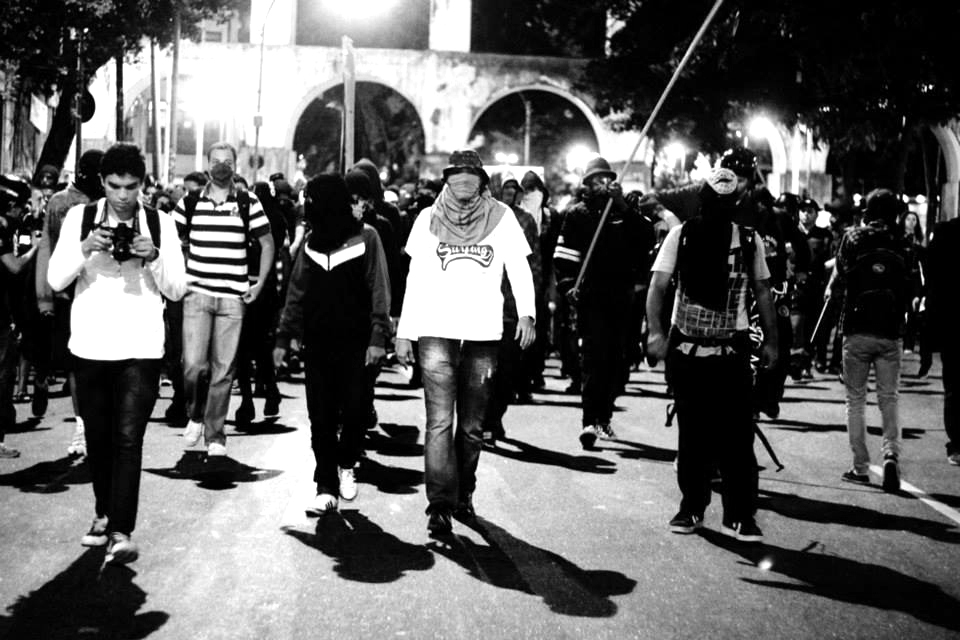
\includegraphics[width=9cm,height=6.1cm]{Imgs/img4.jpg}
\emph{Malta}, 2013
\end{center}

\subsection{Mapa}

Primeiro foi Porto Alegre; depois, Natal, São
Paulo, Goiânia e o Rio de Janeiro. Uma multidão de corpos indóceis e
inúteis impede as vias públicas, para o tráfego eternamente estagnado
das seis da tarde das grandes capitais e, paradoxalmente --- dirão alguns
---, em nome da liberdade de circular insujeitos pela cidade. Quem lhes
teria dado esse direito --- por tanto tempo exclusivo dos automóveis?

Os corpos jovens, liberados e frenéticos que entre 2013 e 2014 ocuparam
as praças e as principais avenidas de grandes cidades em um movimento
metarregional interromperam os fluxos do capital que as sucessivas
isenções de \versal{IPI} tornaram possível. É a potência e a~\emph{virtù~}desses
corpos indóceis e inúteis, insubmissos e nada comportados, que constitui
o princípio de desarticulação das estratégias de poder que se dissimulam
sob a questão da tarifa do transporte público nas grandes metrópoles.
Eis o que torna urgente tentar lançar luzes sobre os protestos que se
espalharam pelo Brasil, para muito além das frases efectistas e
midiáticas, das gritas reativas daqueles que ocupam os postos
discursivos por meio dos quais a grande mídia --- a serviço do Estado e,
sobretudo, dos interesses corporativos --- tenta incessantemente controlar
as margens de crítica social.

As vitrines quebradas --- alvo aparentemente preferido desses corpos
anarquistas --- formam, ao lado das máscaras de Guy Fawkes, de \emph{V
for Vendetta}, e do lixo incendiado,~ o conjunto das grandes marcas
simbólicas --- ou melhor, demasiadamente inconscientes e reais --- das
passagens revoltas dos corpos pelas cidades. Eis alguns dos signos que
permitem produzir uma genealogia dos acontecimentos de superfície que
visa a romper com os quadros de inteligibilidade dados, e enxergar um
pouco além do que, no movimento pelo passe livre e pela tarifa zero,
parece ser meramente acidental. Trata"-se de desentocar a própria
potência política vital de que a coragem crua desses corpos se tornou
depositária.

As vitrines estilhaçadas ---~nem sempre pelos manifestantes~--- nada mais
são do que o acontecimento de superfície de um atentado contra o
princípio de transparência e visibilidade de uma sociedade de controle
em que os corpos são constantemente vigiados nas margens virtuais de
seus gestos; basta um esboço ou um descuido para que o poder que
transforma cada corpo em um sujeito, ou em um indivíduo, torne"-se
sutilmente eficaz e maquinal. Assim, subterraneamente, normalizações vão
moldando cotidiana e continuamente, em um nível infralegal e
parajudiciário, os corpos dóceis e úteis. À luz das patologias da
normalidade que o poder implanta no coração das subjetividades que
produz, tudo o que ameaça a tranquila normalidade do retorno para casa
após um dia extenuante de trabalho só poderia significar um atentado à
liberdade dos ``cidadãos de bem'' --- esses efeitos do poder --- que se
comprazem em se comprimir uns contra os outros nos infinitos
engarrafamentos das metrópoles ou no interior dos coletivos abarrotados;
porém, esta não passa da perspectivação do fenômeno pela sensibilidade
estrábica dos doentes de normalidade, os sujeitos constituídos pelas
finas malhas de poder dos panoptismos que jamais deixaram de integrar as
estratégias das sociedades disciplinares ou de controle. Como as
vitrines estilhaçadas, deixadas para trás pelos corpos revoltos, não
seriam, também, o signo do contrapoder que circula em corpos que se
desejam anônimos, impessoais e inindividualizáveis?

Não se trata de fazer um elogio da violência; trata"-se de evitar
sacralizá"-la nas ilegalidades cometidas pelas Polícias e pelos Estados
pseudodemocráticos --- como o Brasil revela ser. O poder circula pelos
corpos das multidões. Assim como ele explode contra elas, nas ações
criminosas legalizadas em aparência pelas formas jurídicas do Estado e
do capital"-dinheiro, ele também explode~\emph{a partir delas}. É nesse
sentido que Antonio Negri (2006: 50) pudera afirmar que um protesto
pode ser não"-violento, mas jamais será pacífico --- é com o poder que
circula nos corpos que os contrapoderes, até então sujeitados, produzem
sua rebelião profunda.

Esses corpos indóceis usam máscaras. É preciso compreender que para além
da perspectiva da normalidade patológica, o gesto de dissimular o rosto
no espaço público consiste na mais radical afirmação de democracia ---
especialmente quando um Estado que se predica de democrático reprime
qualquer manifestação pública de forma tão sistemática e violenta que
não deixa outra alternativa a seus cidadãos senão a de dissimular o
rosto para ganhar as ruas e ver o enxame amorfo que pouco a pouco
receberá o nome impronunciável, impessoal e politicamente monstruoso de
multidão. Dissimular o rosto: a única forma pela qual essa multidão pode
reapropriar"-se do espaço público quando toda forma de dissidência parece
ter se tornado virtualmente impossível. Tecida apenas de singularidades
impessoais e precárias, é a própria multidão, constituída pela revolta
profunda dos corpos, que relança suas potências, que ocupa as ruas,
negando as identidades que o poder não cessou de tentar fixar sobre seus
corpos agora libertos.

Eis as táticas simbólicas, afetivas e, a um só tempo, inconscientes
mobilizadas a fim de liberar os corpos do jugo normalizante dos poderes
de uma sociedade de controle que ainda conserva muitos dos aparatos de
poder das sociedades disciplinares. Romper sua economia da transparência
(as vitrines, os rostos, as identidades), destruir seu princípio de
registro e controle contínuo (depredar câmeras de segurança ou a
iluminação pública), apor seus signos e palavras de ordem que denunciam
que, no limite, a partição entre o lícito e o ilícito, das formas
jurídicas do Estado, esconde, sob sua superfície verminal, a repartição
maquinal em que o poder seleciona ativamente certas ilegalidades para
receberem a forma legalizadora e o empenho do direito de Soberania. Eis
a macro"-operação de poder capitalística que cobre com o véu da
legalidade o infinito mapa de ilegalidades que essa comunidade de eus
profundos coloca em questão: da máfia dos transportes públicos à das
montadoras de automóveis; da máfia dos empresários do petróleo às
atitudes censoras que constituem a práxis cotidiana da mídia; das
violações de direitos civis que o Estado e a Polícia cometem
sistematicamente às ilegalidades do Direito de exceção que
já vige no país, mesmo antes da realização dos ``grandes eventos'' de
2014 e 2016, aos quais os corpos respondiam com toda a potência de sua
recusa política: ``Não vai ter Copa''.

Quando os corpos destroem o princípio de controle sutil a que se
encontravam submetidos --- as disciplinas infinitesimais que produzem o
sujeito e sua~\emph{belle âme}, que os colam a uma singularidade
orgânica como efeito da insidiosa inscrição desses poderes nos corpos, e
que classificam o bem e o mal, produzem e repartem o normal e o anormal
---, tudo o que resta aos poderes constituídos é fazer valer as
prerrogativas de um direito de Soberania. Isto é, só resta ao Estado
aplicar à massa informe, rebelde e perigosa na qual os indivíduos dóceis
subitamente se converteram às prerrogativas de violência, fiadoras de
primeiro tempo das disciplinas fustigadas pelos contrapoderes que corpos
indóceis e inúteis descobriram sob a superfície artificial e verminal de
seus eus sociais. Assim, o Estado pode transformar"-se em máquina de
abolição completa --- como não raro se transforma --- e fazer da
justiciabilidade dos ``vândalos, anormais e insubmissos'' um
desnecessário e, sob todos os aspectos, injustificável e criminoso
espetáculo de crueldade.

O lixo incendiado é o signo último desse combate. De um lado, a recusa
das dejeções que o sistema de exploração capitalista amontoa e produz
sem cessar; de outro, o princípio incendiário e contaminador que
comunica a indisciplina e a insubmissão como princípio de abertura e
questionamento radical de um corpo a outro; já não podermos falar em
comunicação do aberto entre almas, porque a alma foi queimada com o
fogo. Ela também é, de alguma forma, um dejeto incendiado que o poder
fabricou.

Eis o que todo corpo insubmisso, indócil e inútil que ocupa --- e ainda
ocupará por muito tempo --- os espaços públicos coloca em jogo: um devir
indomável de nossas formas de viver e de pensar para o capital e para o
mercado. Uma forma de reabrir o que parecia fechado, de combater o
fechamento e as estases que o poder produz nos corpos sujeitados.
Impedindo o trânsito violentamente, com a mesma intensa doçura de quem
escreve em um cartaz: ``Desculpe o transtorno. Estamos lutando por seus
direitos'', é o devir de todo um modelo de exercício de poder que esses
corpos jovens, indóceis e inúteis tentam precipitar no aberto. O devir é
o novo, o interessante, o vital que jamais cessa de estar em jogo ---
mesmo quando os corpos cedem ao poder ou se apaixonam por si mesmos. O
devir é o princípio vital, virtual e inorgânico que já se encontra
mobilizado por essas indomáveis existências políticas.

Eis o próprio tempo a colocar em xeque e a afetar irremediavelmente a
totalidade das formas de vida que o poder produziu, e produz, como seus
dejetos cotidianos: sujeitos, restos~\emph{ao lado}. Saímos às ruas e só
encontramos máquinas desejantes, potências selvagens, tesão
político.~\emph{Precipitar as formas de vida no devir}: o que podem
esses corpos rebeldes não é pouco --- sob nenhum aspecto.

\chapter{Contra o rosto}

\begin{center}
\centering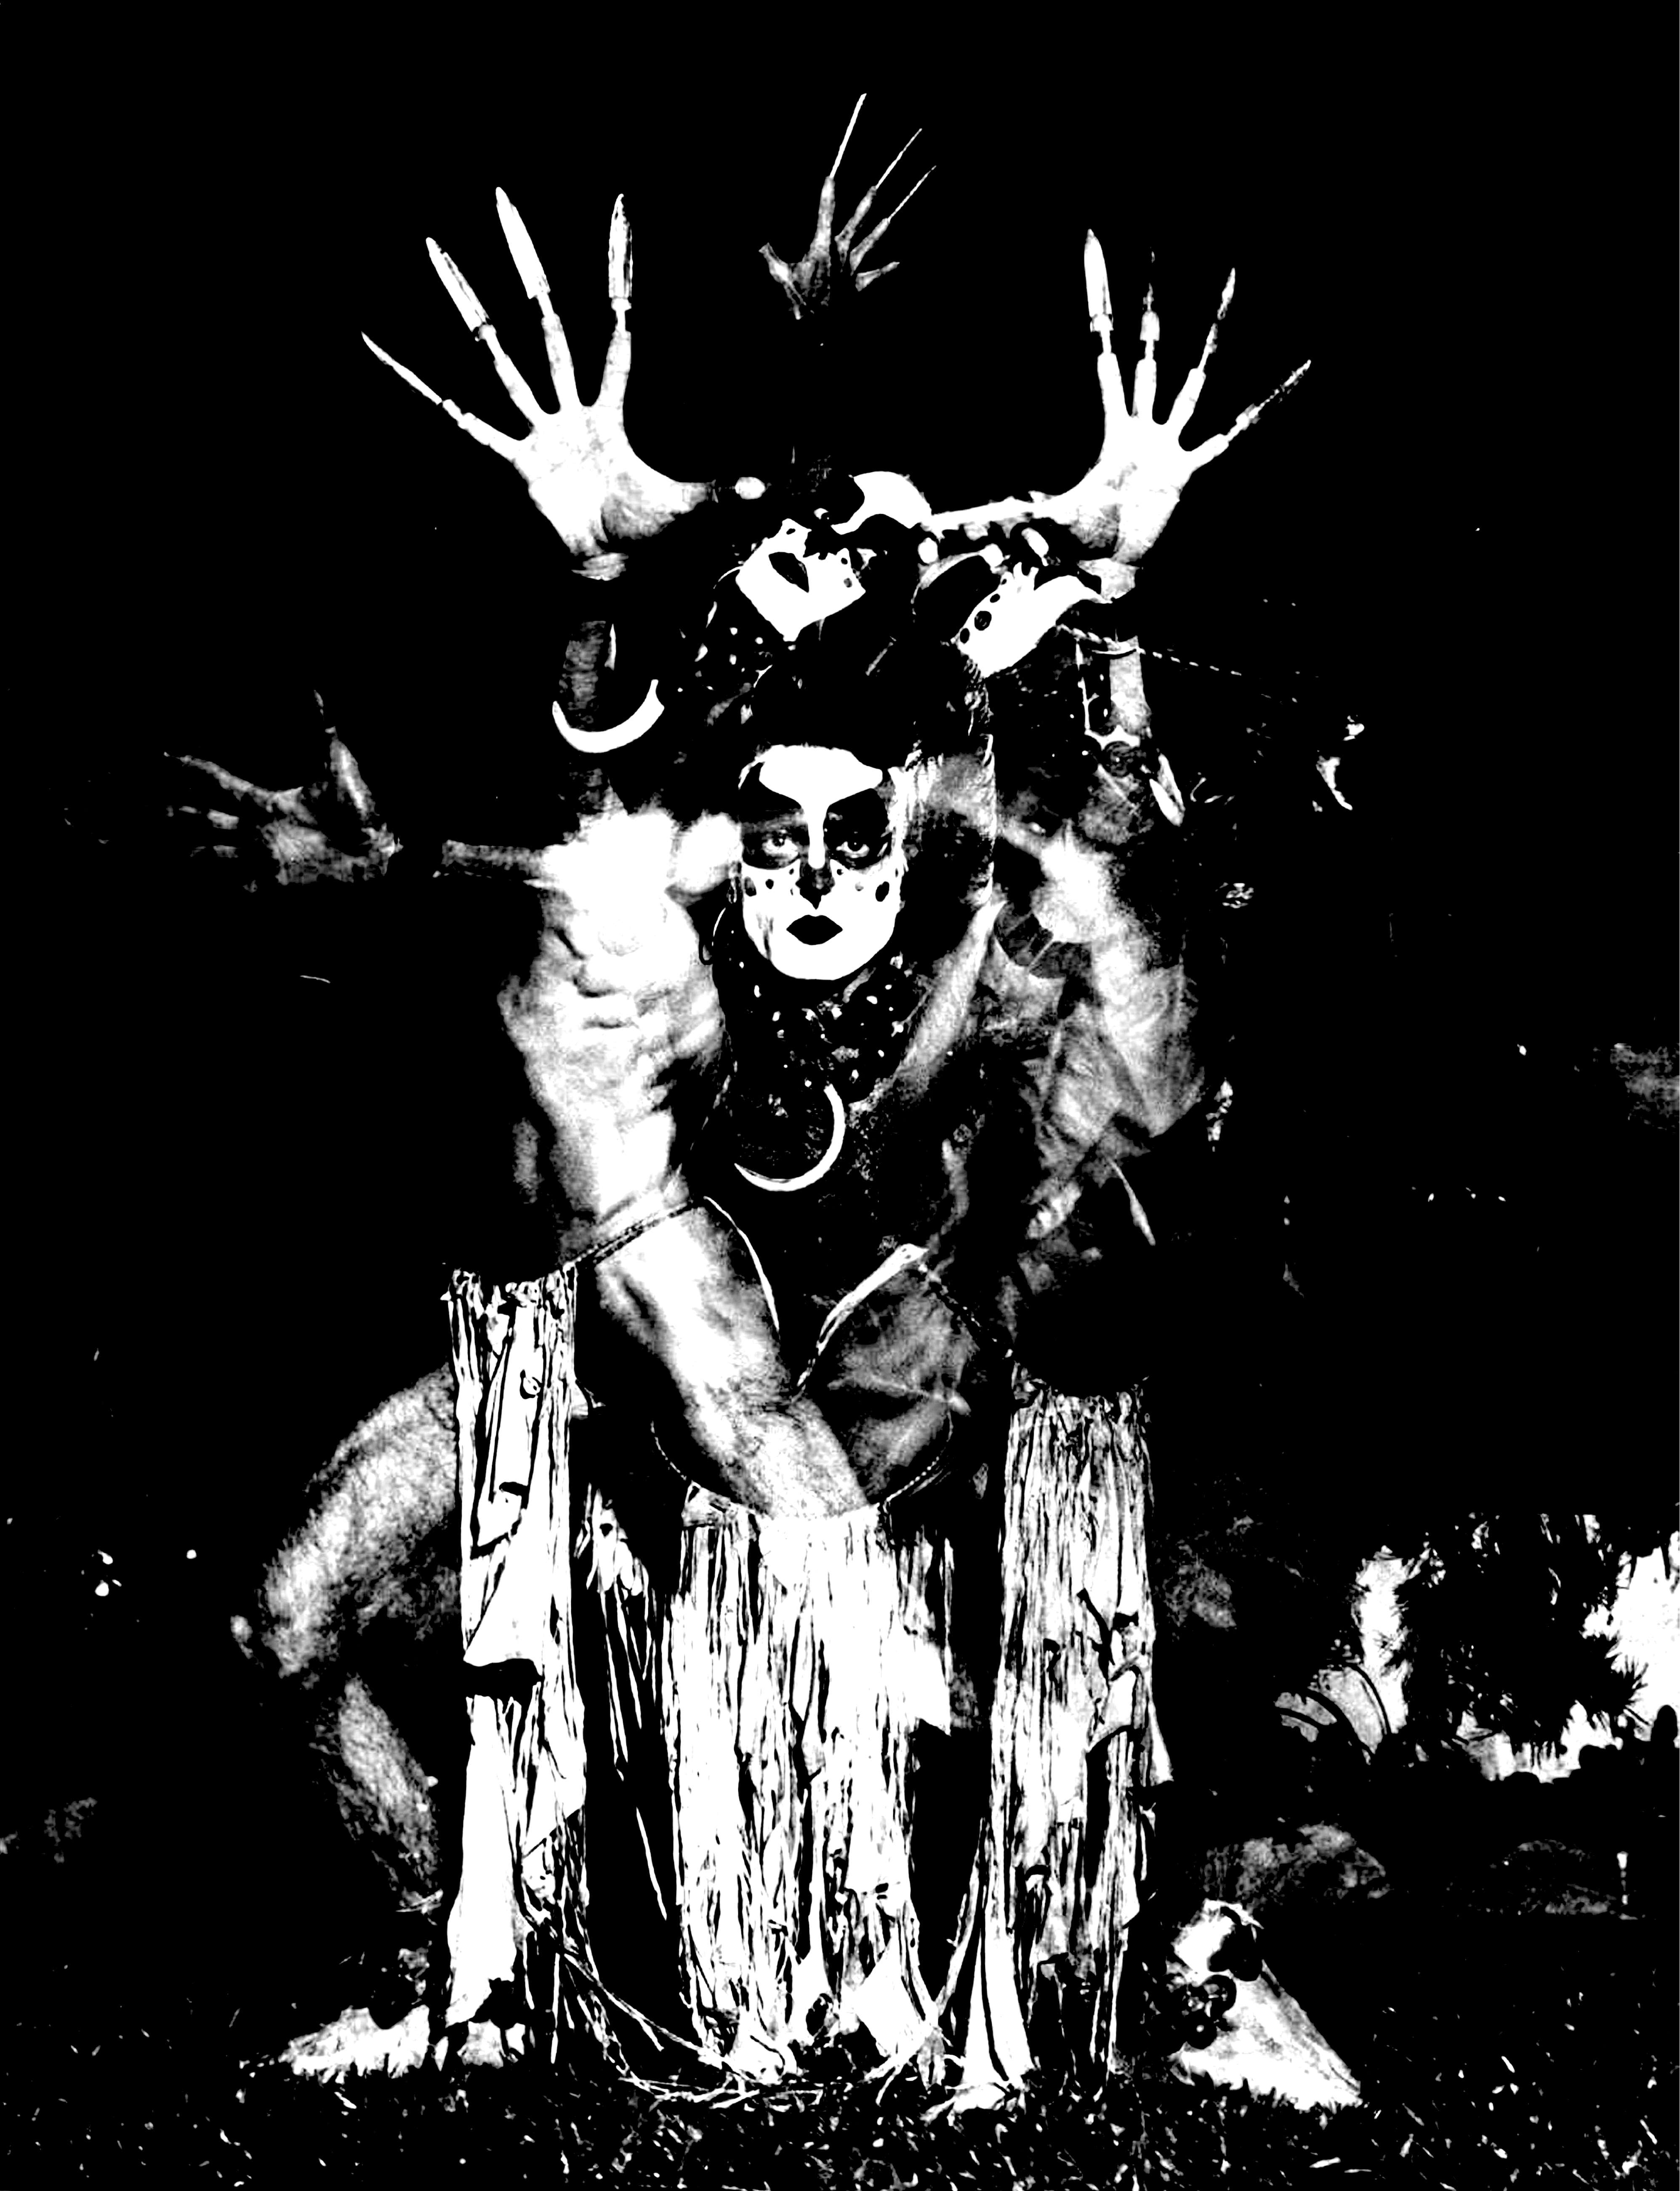
\includegraphics[width=7.245cm,height=11.019cm]{Imgs/img5.jpg}

\emph{Performance}, 1973
\end{center}

\section{E o que me resta é só um gemido}

As sociedades contemporâneas já foram definidas como sociedades
disciplinares, sociedades de normalização e sociedades de controle.
Esses conceitos remetem a uma linhagem que se origina em meados da
década de 1970 nas obras de Michel Foucault e se desdobra em horizontes
conceituais tão heterogêneos quanto aqueles instaurados pelos trabalhos
tardios de Gilles Deleuze, Antonio Negri, Costas Douzinas ou Maurizio
Lazzarato. É da obra desse último que recolhemos a primeira proposição
desse agenciamento \emph{contra o rosto}: ``os indivíduos e as classes
nada mais são do que a captura, a integração e a diferenciação das
multiplicidades'' (Lazzarato 2006: 61). Deleuze (2008: 223) afirma que
seria impossível compreender a passagem das sociedades disciplinares às
sociedades de controle apenas a partir das transformações do capitalismo
--- antes, seria necessário compreendê"-la a partir do que Lazzarato
chamou, na obra de Deleuze, de ``potência da multiplicidade'', que se
confunde com o \emph{fora} que se pretende capturar.

A passagem de um esquema de governamentalidade a outro não é diacrônica
(Foucault 2008: 10; Agamben 2008: 89). Não há transformação simples ou
superação dialética, mas uma sucessão por compenetração, a gênese
temporal e ontologicamente precária de híbridos flexíveis. A emergência
das sociedades de controle --- definidas segundo a difusão imanente dos
dispositivos de controle pela totalidade do campo social (Negri 2008:
39) --- não implica o desaparecimento dos dispositivos disciplinares, mas
a integração das estratégias de controle desenvolvidas durante os
séculos \versal{XVII} e \versal{XVIII} no interior de instituições asilares, hospitalares,
manicômios, escolas e fábricas a partir de outras formas de
governamentalidade das multiplicidades.

As técnicas disciplinares e as formas de governamentalidade biopolítica
incidem de modos diferentes no controle das multiplicidades, que
continuam a ser o seu objeto em comum. Eis o que torna possível que
atuem tanto no plano dos corpos individuais --- como uma anátomo"-política
--- quanto em larga escala, como uma biopolítica das populações (Foucault
2009: 151--152; Douzinas 2013: 33). Isso permite que as estratégias de
poder que atravessam o horizonte epocal da modernidade sejam duais e, ao
mesmo tempo, possam integrar"-se no limiar do século \versal{XX} a fim de
assegurar formas mais totalizantes de sujeição; finalmente, quando suas
sutis estratégias de controle falham, assistimos retornarem os
espetáculos atrozes de violência soberana contra grupos humanos inteiros
--- algo da ordem do suplício ou do soberano exercício do direito sobre a
vida e a morte --- ponto de conversão da anátomo"-política dos corpos ou
da biopolítica das populações em tanatopolítica (Agamben 2007: 129;
Negri 2008: 27). No capitalismo biopolítico, a copresença das formas
de governamentalidade implica uma dupla produção: a produção da sujeição
política e a formação de uma alma cativa, como seu efeito ou dobra
subjetiva.

\section{Minh'alma cativa}

As disciplinas convertem as multidões confusas, inúteis ou perigosas em
classes organizadas por meio de uma estratégia de distribuição de corpos
em espaços quadriculados, clausura, controle da atividade e dos gestos
dos corpos individuais, vigilância virtualmente infinita e sanção
normalizadora. Porém, esse poder não é unicamente externo. Ele
apresenta, como seu correlato, um efeito de subjetivação e
individualização das massas confusas\footnote{A
  individualização tem por efeito diminuir a potência confusa das
  multidões, fixar identidades e tornar indene sua lógica de contágio
  recíproco: ``A multidão, massa compacta, local de múltiplas trocas,
  individualidades que se fundem, efeito coletivo, é abolida em proveito
  de uma coleção de individualidades separadas. Do ponto de vista do
  guardião, é substituída por uma multiplicidade enumerável e
  controlável; do ponto de vista dos detentos, uma solidão sequestrada e
  olhada'' (Foucault 2012: 190).}. Numerosos dispositivos de
enclausuramento (prisão, escola, caserna, hospital, fábrica) definem"-se
como um corpo a corpo entre sujeitos e aparelhos que atuam sobre
multiplicidades pouco numerosas, distribuindo"-as e seriando"-as a fim de
recompô"-las no espaço, diminuindo em cada um dos corpos a potência de
rebelar"-se e aumentando sua sujeição, docilidade e utilidade.

As técnicas biopolíticas, que incidem sobre fenômenos heterogêneos de
grande escala (mortalidade, natalidade, escassez alimentar, desnutrição
etc.), exercem"-se de outra maneira, supondo um espaço aberto, ilimitado,
que abrange os corpos individuais apenas na medida em que eles pertencem
ao corpo biopolítico da espécie e da população. Nesse caso, é preciso
definir uma outra forma de divisão que, já não sendo tão
individualizante, não deixa de forjar um campo de subjetivação como
correlato das relações de poder que atravessam e formam populações
inteiras --- uma maneira de alienar a irredutível potência das
multiplicidades ao Um.\footnote{Essa forma de
  subjetivação, no caso da biopolítica das populações, pressupõe que os
  limites da população sejam definidos pela nação (Lazzarato 2006: 65).}

Nesses campos de relações de forças intrincadas e heterogêneas, não há
exercício de poder que não tenha como correlato a produção de alguma
dimensão de subjetividade (Foucault 2012: 32). Exemplar disso é que, na
teoria jurídica moderna, o exercício do poder de soberania não cessa de
subjetivar os indivíduos como súditos ou sujeitos de direitos; o
exercício do poder disciplinar subjetiva segundo a repartição entre o
normal e o desviante; os dispositivos biopolíticos subjetivam elementos
de cálculo governamental no corpo de massas humanas inteiras e
homogêneas segundo o binômio cidadão/não"-cidadão, o que equivale à
repartição do comum dos seres humanos entre pertencentes e
não"-pertencentes ao corpo biopolítico da população de um Estado. A mesma
operação não cessa de apresentar"-se no campo das ciências humanas. Todas
as tecnologias da alma, da psicologia à antropologia, oferecem um
\emph{anthropos} a ser liberado que é, já, um efeito de poder exercido
sobre os corpos. Sob todo exercício de poder e sujeição insistem
processos de subjetivação como seu correlato. Em síntese, o poder se
exerce sempre sobre multiplicidades, mas atua de tal maneira que cria
sempre uma identidade de maior ou menor escala --- uma alma ou o corpo
biopolítico de populações inteiras --- como efeito desse poder.

Encontramos aí, nesses sujeitos ou grupos, o artifício com que os
poderes moldam desde massas inteiras de cidadãos anônimos --- as massas
confusas, inúteis e perigosas, de Foucault --- sem deixar de atuar sobre
o mais fino grão dos indivíduos, criando uma alma, uma consciência, uma
\emph{psique} para cada corpo. Eis o que torna as sociedades de controle
eficazmente difusas e modulares. Capazes de exercer controle em
praticamente qualquer espaço, seus dispositivos vigiam desde as massas
anônimas e anárquicas até as rugas de um rosto na multidão; com a mesma
naturalidade de quem dá \emph{zoom} em uma câmera de videovigilância
superpotente, as sociedades de controle abrangem virtualmente, e a um só
tempo, os conjuntos totais e a menor partícula, domesticam diferenças
macro e micropolíticas.

Assim como os sujeitos --- suas identidades e almas --- não passam de um
efeito das relações de poder que atravessam seus corpos, seus rostos ---
que não se confundem com a sua cabeça ou com seus corpos --- são apenas
suas máscaras disciplinares ou biopolíticas. Os corpos são sutil, mas
indelevelmente, marcados com o selo de uma forma de exercício de poder
que funde e difunde sobre toda a extensão do tecido biopolítico esses
diferentes modos de exercer o controle sobre as multiplicidades das
vidas e dos corpos. Imanente à totalidade do campo social, o exercício
de poder nas sociedades de controle deixa de ser unicamente vertical,
embora ainda possa encontrar no Estado e nas instituições sociais alguns
de seus atores privilegiados --- máquinas que terminam por polarizar, em
determinados momentos, as gramáticas das relações de poder.

De todo modo, encontramos aquilo que a análise microfísica do poder de
Foucault descrevia já em meados dos anos 70:

\begin{enumerate}
\item O poder é sempre uma
relação de forças --- eis o que define sua horizontalidade e imanência,
como a possibilidade de contrapoderes e contracondutas (o polo
ontologicamente anterior a qualquer formação de poder: a resistência)
(Deleuze 2014: 207--208);
\item O poder incide sobre o corpo, e o sujeita
ao mesmo tempo em que o subjetiva;
\item A produção de subjetividade advém
tanto do exterior quanto do interior --- isto é, não apenas a linha dura
e segmentar dos poderes que penetram os corpos criam um sujeito para
eles, mas, em seu seio, não é possível haver subjetivação sem criar, ao
mesmo tempo, resistência à linha dura que vem de fora, que cria um
corpo, mas também uma alma e um rosto, no qual se territorializa sempre
uma multiplicidade a controlar.
\end{enumerate}

Se observarmos as emergências das manifestações populares --- renascidas
em junho de 2013, a partir do Movimento Passe Livre (Judensnaider et
al. 2013), em seguida arrefecidas e retomadas no início do mês de
setembro com uma potência nova, junto à manifestação de professores da
cidade do Rio de Janeiro, veremos a operação fluida desse tipo de
mecanismo ganhar um aparente corpo institucional. Os aparelhos de Estado
impõem progressivamente algumas estratégias para tentar fixar as
subjetividades das multidões indecisas em função da produção de
identidades e rostos. Não podendo mais ignorar as multidões nas ruas das
maiores cidades do Brasil, os oligopólios da mídia produzem velozmente
uma estratégia de disciplina simbólica que visa a promover a divisão
politicamente útil entre o manifestante pacífico e o manifestante
violento. Na medida em que o manifestante violento é paulatinamente
identificado com os garotos que se utilizam da tática black bloc, a
estratégia passa a ser aprofundar ainda mais a cisão entre o
manifestante pacífico e o violento de duas maneiras isométricas: ora
identificando o manifestante violento com a figura socialmente
naturalizada do criminoso desprovido de direitos, ora identificando o
black bloc --- que não é um grupo de pessoas, mas verdadeiro agenciamento
temporal, kairológico e precário --- como coletivo.

Na medida em que se pode identificar um coletivo, a polícia persegue o
que supõe serem organizadores ou líderes de um acontecimento político
que se define pela horizontalidade, pela dissolução da identidade
individual e pela acefalia --- isto é, pela potência imanente aos
próprios corpos. De outro lado, o Estado, a fim de garantir que a
polícia possa responsabilizar os indivíduos que fazem parte das ações
black bloc, passa a proibir por lei a dissimulação do rosto em
manifestações populares.

Eis o ponto em que encontramos não apenas a articulação entre
estratégias de poder e de subjetivação, mas, sobretudo, a clara
interpenetração de estratégias de biopoder que compreendem heterogêneos
e integrados modos de exercício do poder sobre os corpos: a soberania
manifesta"-se na lei e na violência; a disciplina, na conversão semiótica
do black bloc a criminosos comuns; o biopoder, no bloqueio maciço e
simbólico à variação biopolítica das formas de vida que o black bloc
reivindica ativamente sob a forma de uma agressiva recusa do capital e
do Estado.

Chegamos ao ponto duplamente interessante em que as multidões indóceis
--- os corpos anarquistas e sem rosto das ruas --- coincidem com o objeto
de que o poder quer se assenhorear, cuja potência política quer
neutralizar, cujo rosto quer inventar (e, em sentido etimológico,
invenção é, também, apropriar"-se, assenhorear"-se), e cujas
singularidades precisa organizar sob uma forma jurídica criminalizável.
O poder não se exerce senão em correlação com sucessivas formações de
subjetividade, atribuições de identidades e feições, semióticas e
símbolos sempre dispostos à hipocrisia ou à perversão dos tribunais
morais, justamente porque formar uma identidade por meio da qual se
torne possível assenhorear"-se da potência de um corpo --- ou, pelo menos,
neutralizá"-la temporariamente --- consiste em uma espécie de meio caminho
para a dominação.

Em 11 de setembro de 2013, o governador do Rio de Janeiro, Sérgio
Cabral, sancionou o inconstitucional\footnote{À luz dos
  incisos \versal{IV} e \versal{XVI} do artigo 5º da Constituição da República, bem como
  do artigo 23 da Constituição do Estado do Rio de Janeiro, fica
  bastante claro que os poderes constituintes da República e estaduais
  não atribuíram qualquer competência aos poderes legislativos federal e
  estadual para regulamentar restritivamente os direitos fundamentais à
  livre manifestação de pensamento e à livre reunião. O único
  condicionamento formal à liberdade de reunião é administrativo, e
  consiste no ``prévio aviso à autoridade competente''. A
  inconstitucionalidade formal da Lei Brazão é, portanto, evidente. Para
  além disso, se a Constituição da República condicionou o exercício do
  livre pensamento à vedação do anonimato, foi a fim de impedir a
  ausência de identificação em documentos e escritos --- princípio útil à
  potencial responsabilização jurídica de seus autores. Porém, um
  manifestante cessa, por manter seu rosto coberto, de ser
  identificável? Evidentemente, não, na medida em que nos termos do
  inciso \versal{LVIII} do artigo 5º da Constituição da República, ele deve estar
  civilmente identificado --- isto é, deve portar seus documentos de
  identificação civil~---, ou poderá ser conduzido pela polícia para que
  seja realizada sua identificação criminal. Como se vê, o manifestante
  de rosto dissimulado e a condição de anonimato não coincidem
  absolutamente; ao contrário, indicam dois institutos diferentes.
  Todavia, o esforço das instituições policiais e da mídia em
  identificar anonimato e dissimulação do rosto, revela, finalmente, o
  escopo criminalizante que insiste isomorficamente sob a identidade que
  funda o que Foucault chamou de ``função"-autor'' em nossa cultura: a
  possibilidade de apropriação penal de textos e escritos, no caso da
  autoria (Foucault 2001: 827), que, entre nós, revela"-se na
  possibilidade de apropriação prisional dos corpos, no caso da ação
  política.} projeto de Lei Estadual nº 2.405/2013 que pretende
proteger ``O direito constitucional à reunião pública para manifestação
de pensamento {[}\ldots{}{]}''. Para tanto, determinou ser ``{[}\ldots{}{]}
especialmente proibido o uso de máscara ou qualquer outra forma de
ocultar o rosto do cidadão com o propósito de impedir"-lhe a
identificação.'' Mais adiante, a mesma lei condiciona o exercício do
direito à reunião pública e manifestação de pensamento à não"-utilização
de ``máscaras nem de quaisquer peças que cubram o rosto do cidadão ou
dificultem sua identificação'' --- regra excepcionada no caso de
``manifestações culturais estabelecidas no calendário oficial do
Estado'', como o Carnaval do Rio, e.\,g. Dessa maneira, o Rio
entrava para um grupo de cidades ao redor do mundo que --- por razões de
segurança nacional, prevenção ao terrorismo ou proteção internacional
aos Direitos Humanos --- possuem legislações que proíbem a dissimulação
do ``rosto do cidadão'' no espaço público.

O primeiro país europeu a editar uma lei que proibia a dissimulação do
rosto no espaço público foi a Bélgica, sob o contexto da discussão
acerca da proibição do uso da Burca e do Niqab pelas mulheres
muçulmanas no espaço público. Se a Lei Brazão importa uma exceção às
Constituições da República e do Estado do Rio, a lei belga derivou de
uma simples positivação legislativa de regras que já preexistiam como
regulamentos de polícia vigentes em praticamente todas as comunas belgas
e que vedavam, ``por razões de ordem pública'', circular em vias comuns
com o rosto encoberto. Em julho de 2010, na França, a Assembleia
Nacional alterou o Código Penal francês a fim de proibir a ocultação do
rosto no espaço público. O argumento dos defensores da medida procurava
seu fundamento no direito das mulheres muçulmanas radicadas na França de
coabitarem no espaço público com seus rostos livres das constrições da
tradição muçulmana, que lhes impunha o véu e a dissimulação do rosto.
Eis porque a lei ficou conhecida como ``lei do véu'' ou ``lei da
burca''. Porém, a despeito de todo o contexto de produção dessas medidas
legislativas, tanto a lei belga como o projeto francês interditam
simplesmente a ocultação do rosto com o uso de vestimentas no espaço
público; nada mais.

Em todos os casos, a proibição da dissimulação do rosto no espaço
público vincula"-se sempre, de algum modo, a conteúdos identitários ---
seja a conteúdos culturais formadores de identidade de grupo (direitos
humanos, papel social da mulher, direito à igual dignidade), seja a
conceitos jurídico"-políticos fundantes da subjetividade biopolítica ---
como a noção de cidadania --- mais diretamente relacionados com a
política de assimilação de estrangeiros e a persistente sombra do
terror. Portanto, quando a Lei Brazão condiciona o exercício do direito
constitucional à reunião pública e livre manifestação de pensamento à
não"-dissimulação ``do rosto \emph{do cidadão}'', será preciso considerar
essa expressão \emph{à la lettre}.

Eis o ponto que revela o significado profundamente político da Lei
Brazão; ela engendra um dispositivo de poder comum a todas as leis que
proíbem a dissimulação do rosto no espaço público e mantém sua relação
com a anulação dos perigos que os corpos sem rosto comportam ou
traduzem.

A lei que interdita o direito de dissimular o rosto no espaço público
coloca em xeque o significado profundamente biopolítico do rosto e de
sua relação com os corpos e sua potência. Como o Estado faz do rosto uma
política de subjetivação e, ao mesmo tempo, de controle dos corpos? Se
quisermos responder a essa questão, é preciso compreender o que é um
corpo, o que é um rosto e como o rosto pode se tornar um elemento"-chave
na dominação dos corpos.

\section*{Quebrei a lança, lancei no espaço: um grito}
\addcontentsline{toc}{section}{Quebrei a lança, lancei no espaço}

Embora não se confunda com ele, o corpo pode passar integralmente pelo
rosto. Na medida em que o rosto é produzido a partir de elementos de
subjetividade, mas também de paisagem, um corpo pode ser inteiramente
rostificado (Deleuze e Guattari 2008: 35). O corpo remete ao um código
polívoco multidimensional; ou melhor, ele remete à descodificação, na
medida em que jamais se pode saber \emph{a priori} ``o que pode um
corpo''. A determinação de sua potência é da ordem contingente dos
encontros, da formação de afetos, da variação de sua potência de agir. O
rosto, porém, na medida em que recobre a cabeça, em que separa a cabeça
do corpo, os sobrecodifica. Na operação de rostificação, toda a potência
de um corpo é alienada ao vazio e ao tédio unidimensionais do rosto,
enquanto o semblante corporifica uma formação codificada. Fazer o corpo
passar pelo rosto é uma forma de apagá"-lo enquanto tal, de remetê"-lo ao
despotismo de um significante: dois olhos, um nariz, uma boca, orelhas
--- jogo de superfícies e buracos, \emph{close} e sombras organizadas
para significar.

Procuremos compreender o que Deleuze e Guattari querem dizer quando
afirmam que ``O rosto é uma política''. Nas formações sociais ocidentais
modernas e contemporâneas, o Estado implanta uma máquina de rostificar
ao lado do corpo social; máquina que se apodera dele, que o rostifica
inteiramente, reduz corpos a rostos, fixa singularidades metaestáveis a
identidades fixas. O rosto é, sobretudo, o análogo, no corpo, da divisão
mais profunda entre sociedade e Estado. O rosto aliena a potência dos
corpos da mesma forma como o Estado aliena o poder do corpo social ---
poder no qual as multidões das ruas nos fizeram submergir como no mais
profundo de nós mesmos. Segundo essa divisão, o corpo deve confinar"-se
ao privado --- espaço em que também os prazeres do sexo, ou os desvarios
do desejo, devem permanecer confinados; o rosto, porém, pertence ao
público, como signos da sexualidade ou do desejo que podem aparecer em
um semblante, portador de índices significantes. A divisão corresponde,
sempre, à sobrecodificação dos corpos em uma ordem espacializante. Os
corpos impotentes, inermes e rostificados são confinados ao espaço
privado; enquanto isso, o Leviatã --- que deseja eclipsar nas suas
instituições a totalidade do espaço público --- torna"-se ``o corpo de
corpos'' que define a unidade identitária à qual se subsumiria o espaço
público, na modernidade.

Os aparelhos de Estado funcionam como uma horrível cabine de
\emph{instant photos}: assinalam e atribuem a identidade unívoca de cada
corpo e, reduzindo o corpo ao rosto, conjuram a multiplicidade confusa
das multidões indóceis, anulam o elemento ontológico e político
irredutível que constitui sua potência específica: ser um corpo no qual
nada se assemelha a um rosto, uma diferença livre na qual nada se
concilia com tecnologias identitárias. Os primitivos cobriam"-se de
máscaras para atestar a pertença da cabeça ao corpo; os contemporâneos o
fazem sempre em fuga, para converter os rostos em cabeças"-pesquisadoras
(Deleuze e Guattari 2008: 61).

O Estado identifica mascarado e criminoso sob o signo da culpa \emph{a
priori }(segundo o léxico do poder, ``se esconde a identidade, é porque
está devendo --- e covardemente\ldots{}''). Serve"-se da perversa naturalização
da categoria do criminoso, pois, assim, pode"-se negar"-lhe direitos,
capturando"-o em um espaço exterior ao direito. Justamente por isso,
Amarildo --- o pedreiro torturado, morto e cujo cadáver foi ocultado pela
Polícia Militar do Estado do Rio de Janeiro --- não foi logo acusado de
colaboração com o tráfico? O crime --- exceção prevista na ordem jurídica
--- cria o universo simbólico bastante para justificar perante a opinião
pública toda a violência policial estrutural --- a exceção não"-prevista
como estratégia de controle dos corpos.

Capturado fora das leis que assinalam o hipnótico pacto social, a
coincidência entre o mascarado e o criminoso é o sintoma mais
superficial da profunda crise desse ``contrato''. O efeito simbólico e
político do retórico ``recurso ao pacto'' é alienar toda possibilidade
de pensamento ao código de suas razões, fazer"-nos abdicar da crítica,
que Foucault (1990) definiu como ``a arte de não ser governado assim e a
tal preço''. Desfazer o seu próprio rosto, no Brasil atual, é resistir a
abdicar da faculdade de pensar --- não é nada fácil e implica o risco de
ter, de novo, um corpo implicado na política ou na prisão.

No campo instável e aberto da ``baderna'' e da ``subversão'', a polícia
--- e seus antigos aparelhos jurídicos de Segurança Nacional, jamais
formalmente revogados --- tornam"-se o instrumento por excelência de
governamentalidade para controlar situações fluidas, metaestáveis e de
emergência. Isso porque a polícia e seus aparatos técnico"-sociais, como
as mídias e a videovigilância, são capazes de restabelecer as
identidades, de reatribuir o rosto a quem ousou desfazer"-se dele. Ao
mesmo tempo, a micro"-mídia, como a Mídia Ninja e.\,g., ensaiou, nos
primeiros dias, uma dinâmica contra"-hegemônica: transmitindo a
insurgência das multidões via \emph{live stream}, acompanhando e
denunciando ao vivo situações de abuso policial, com apoio das redes
sociais, mas sob a constante ameaça de violência e encarceramento.

``A cada corpo, seu próprio rosto'' é a injunção do Estado, e tudo o que
coloca em xeque a ordem das coisas é violentamente conjurado. Nada de
massas confusas, nada de corpos anarquistas e indisciplinados, nada de
multidões sem rosto: mesmo fora de qualquer conceito de
organização, o Estado continua a afirmar e enquadrar tudo
o que ensaia sua fuga como organização ``informal'', ``disforme'', mas
inequivocamente ``criminosa''\footnote{``Polícia vai
  enquadrar vândalos em nova lei de organização criminosa.'' \emph{O Globo}, 08/10/2013.}. Nesse caso, ``Manifestação pacífica''
coincide, ponto por ponto, com a abolição da política; coincide com a
aderência ao rosto e aos afetos da ordem, quando toda política é, no fim
das contas, a possibilidade de criar uma outra ordem dos afetos. Toda
ação política que combata a ideologia que aliena e sacraliza a violência
como prerrogativa exclusiva de um Estado violento e de uma polícia
assassina deve ser violentamente conjurada, pois desafia o Um, a
sociedade dividida entre dominadores e dominados, ricos e pobres,
exploradores e explorados, alienação do poder do corpo social ao Um
transcendente do Estado.

O que define a verdade profunda das multidões --- o que as subjetiva como
tal --- é a recusa ativa do rosto em proveito das singularidades
irredutíveis de um corpo social criativo, múltiplo, nômade, anônimo,
potente, inclassificável e incoercível. O rosto é uma política --- e
desfazê"-lo é nosso destino --- porque no seio de uma cultura metafísica e
política identitária, a política é, antes de tudo, uma guerra de
guerrilhas entre corpos indisciplinados e rostos despóticos.

Por essa razão, as máscaras podem desempenhar, ainda hoje, a função que
tinham para os primitivos que, muito antes de Nietzsche ou de Foucault,
conheciam a guerra como relação social fundamental. Como atesta Pierre
Clastres (2011: 236), a função da guerra nas sociedades primitivas era
a de conjurar o aparecimento da forma"-Estado na chefia, da sociedade
dividida, da conversão irracional de suas sociedades de abundância e de
lazer em sociedades"-para"-a"-acumulação. As sociedades primitivas são
sociedades contra"-o"-Um: sociedades centrífugas, que perseveram no seu
ser"-para"-o"-múltiplo.

Instaurada uma máquina de rostificação, uma correlação de forças se
estabelece entre dispositivos que querem atribuir a cada corpo um Rosto
e entre singularidades que resistem à identificação e instauram uma
micropolítica da invisibilidade: cobrem o rosto para se verem livres,
pelo menos temporariamente, do controle virtualmente infinito, contínuo
e insidioso dos aparelhos de Estado e das tecnologias que lhe são
correlatas.

O Estado e o rosto são os antípodas da política --- antes uma máscara
diabólica para assegurar uma cabeça bem atarraxada ao corpo que o rosto:
máscara biopolítica. No Brasil, as ruas assinalam muito mais que uma
acumulação primitiva de democracia; marcam, em coextensão com ela, a
emergência de uma nova noção de espaço público, completamente emancipada
do Estado e para além de sua métrica: desejo de desfazer o rosto, de
multiplicar o múltiplo, de ser contra"-o"-Um.

\section{«Não tinha rosto. Eu oferecia meu corpo»}

Estamos em 1973. Um corpo esguio, seminu e frenético dança na televisão.
Ao ritmo quatro por quatro do \emph{rock ``}Sangue Latino'', os quadris
e o abdômen se movem como moinhos --- mas não graças aos ventos do norte,
ou à sua transcendência. O corpo é mais que uma presença: é uma
performance. O rosto está inteiramente despedaçado sob uma pesada
máscara \emph{kabuki} de tinta e pó. A lógica da rostidade,
buraco"-negro/parede"-branca, é conduzida ao limite imanente do corpo.
Nariz, olhos e boca são, agora, apenas linhas de força contra o muro. Os
buracos"-negros são ainda mais negros e parecem se chocar, ou dançar,
como um grafite sobre uma enorme parede branca. A boca é um buraco"-negro
que se fecha e abre. Em perfil, os ombros se curvam e encolhem na
direção da cabeça tornando"-a indiscernível do corpo. Indefinidamente sem
rosto, a cabeça se continua na intimidade exposta de um corpo seminu. As
longas penas sobre a cabeça que percorrem a extensão do corpo, ao mesmo
tempo em que o delimitam, não cessam de remeter a um devir"-índio,
lobisomem ou pirilampo.

Ontologia política dos Secos \& Molhados: se o rosto é uma política, e
se as máscaras dissolvem as identidades, tudo o que resta sob elas é uma
multiplicidades de corpos anárquicos, frenéticos e indomáveis. Secos \&
Molhados compreenderam com precedência a natureza biopolítica do rosto,
as estratégias disciplinares que envolviam o processo de rostificação e,
nesse sentido, apareciam no kairológico ano de 1973 como o primeiro
grupelho disposto a depor o despotismo do rosto que a ditadura
brasileira --- e sua polícia política --- queriam inventar.

Os corpos e as máscaras contra o rosto. Nem as máscaras indicavam o
rosto, mas a insistência da cabeça, nem o corpo denunciava o indivíduo,
mas o dissolvia e convertia em um ponto de passagem violenta de uma
força da natureza: o devir contra o tempo cronológico e os espaços
quadriculados da disciplina e do biopoder. Ainda que seus eus o
ignorassem, os Secos \& Molhados formaram o primeiro black bloc ---
vandalismo significante, ação direta contra o rosto (a propriedade
primeira, já que, antes do nome, temos um rosto), confusão das
identidades, multiplicação dos gêneros e explosão infinitesimal dos mil
sexos.

Quase quarenta anos mais tarde, Ney Matogrosso --- o nome próprio e o
rosto familiar --- explicaria que foi a Liberdade, bairro paulistano
povoado pelos imigrantes e pela cultura japonesa, que inspirou a criação
de suas máscaras.\footnote{``{[}\ldots{}{]} eu já pensava em
  desenhar no meu rosto uma máscara. Fui numa casa de maquiagem para
  teatro e comprei potes de tinta branca e preta. Me inspirei nas
  imagens no teatro ``kabuki'', que para mim eram muito fortes, e com as
  quais tive contato no bairro da Liberdade, quando morava em São Paulo.
  Passei a me apresentar mascarado, porque tinha muito medo da
  exposição. Ouvia dizer que artista não podia andar na rua. Eu tinha
  pavor de perder esse direito. Na medida em que fui observando o
  aumento da receptividade ao Secos \& Molhados, fui fechando a máscara
  no meu rosto. Eu não permitia que publicassem fotos minhas sem a
  pintura. Foi uma atitude.'' Revista \emph{Brasileiros}, 01/08/2013.}
Ao mesmo tempo em que o tímido e esguio rapaz desejava preservar sua
identidade --- pois não queria perder a liberdade de andar na rua --- a
máscara era, também, a única maneira para ter
coragem\footnote{``No momento que fiz aquela máscara no
  rosto, adquiri superpoderes\ldots{} Eu, que sempre fui uma pessoa
  tímida, inibida, regatada, não sei mais o quê, deixei de ser tudo
  isso. {[}\ldots{}{]}. Era incapaz de trocar de camisa na frente de
  alguém. Vivia com as mãos no bolso, porque tinha vergonha delas.''
  Ibidem.}
e sustentar a atitude \emph{rock} das baladas \emph{pop }que embalavam
os textos poéticos de João Ricardo, o principal compositor de Secos \&
Molhados. Mascarado, Ney Matogrosso afirmava que ``Não tinha rosto. Eu
oferecia meu corpo''. O real do corpo contra o significante do rosto; o
devir e o \emph{kairós} do encontro contra o espaço quadriculado das
disciplinas, ou o tempo mensurável do biopoder dos militares e suas
fábricas de desaparecer com corpos --- que se tornam atualmente visíveis
no desaparecimento de Amarildo e no encarceramento de Rafael Braga
Vieira, morador de rua da cidade do Rio, detido no protesto de 20 de
junho de 2013 e condenado à prisão por ``porte de artefato explosivo''
--- duas garrafas plásticas com álcool etílico e água
sanitária.\footnote{``Catador é o
  primeiro condenado após protestos.'' \emph{Folha de S.\,Paulo}, 04/12/2013.
  Ainda, sobre o caso Rafael Braga Vieira, cf. \versal{CORRÊA}, 2018.} Rafael
é o primeiro condenado pelos protestos de junho --- signo de que não
apenas jamais abandonamos as prisões políticas, como de que toda prisão
é radicalmente política.

\asterisc

Em um de seus últimos textos, Foucault (2001: 1527) dizia que a
infelicidade dos homens jamais pode ser um resto mudo da política; a
infelicidade dos homens funda um direito absoluto de se insurgir e de
interpelar aqueles que detêm o poder. Surdamente, o direito absoluto de
se insurgir torna mais uma vez visível, sob as formas jurídicas, uma
ontologia jurídica espinosana, segundo a qual o direito não pode
definir"-se senão por aquilo que os corpos podem: sua potência de agir e
de compreender, de agenciar"-se, afetarem"-se e criar novas formas de
liberdade e de resistência.

Uma tal ontologia jurídica define"-se pelo amor de que os corpos são
capazes, do qual as máscaras biopolíticas são apenas testemunhas frias.
O direitos humanos não são mais do que a faceta instituída desse amor ---
frutos da revolta, memória para o porvir (Lapoujade 2010: 93) que
lembra os corpos daquilo que eles podem. Os direitos humanos só podem
deixar ser o que foram para a tradição e o cânone, universais abstratos,
se forem religados à memória do intolerável, da insurgência e da
revolta.

A potência específica do black bloc está em reatualizar a ontologia
política dos Secos \& Molhados: ``Não tinha rosto. Oferecia meu corpo''.
Contra o rosto --- a propriedade primeira~---, suas ações diretas são
verdadeiros \emph{happenings} inorganizados, a não ser, talvez, pela
mediação de simulacros que jamais prefiguram uma identidade de grupo,
pois são todos atos absolutamente \emph{comuns}, dividuais, difusos no
espaço, mas atualizados no tempo simultâneo da ação direta (comunhão
ideológica, gestão de perfis e compartilhamento de informações em redes
sociais, formas de ação, indumentária preta e dissimulação do rosto).

A tática black bloc comporta uma etologia pós"-humana da ordem das
contracondutas ou da indisciplina; sua ética recusa, contesta e destrói
a cronologia das relações de poder constituídas --- os espaços
individuais bem determinados da era disciplinar --- com uma potência
kairológica de um tempo de compenetração. Contra sua captura imóvel em
uma atualidade absoluta, os corpos supranumerários dissolvem seus rostos
e identidades; abandonam os espaços quadriculados aos quais os poderes
gostariam de conformá"-los e escapam, ainda que por um entretempo, à
pertença ao corpo biopolítico das populações que lhes fora destinada. O
rosto dissimulado é sempre o do cidadão, repete a Lei Brazão. Não sendo
mais cidadãos, não são mais homens --- e sabemos, como Arendt (2009:
333) e Agamben (1996: 25), que nos esquemas do Estado"-Nação o homem
jamais deixou de ser o pressuposto mais ou menos evanescente do cidadão.
Ocultado ou dissolvido o vínculo jurídico"-político de cidadania, resta a
inumanidade e o abandono à morte violenta, mas, ao mesmo tempo, a
potência de inventar novos modos de existência para corpos inconformados
e informes. A recusa da máscara biopolítica, que por tanto tempo se
confundiu com seus rostos é, também, a primeira afirmação de uma \enlargethispage{\textheight}
multiplicidade qualquer --- modo de subjetivação singular e
\emph{contra"-o"-Um} que define o sentido genealógico da política na
democracia.

\chapter{Filosofia dos corpos misturados}

\begin{center}
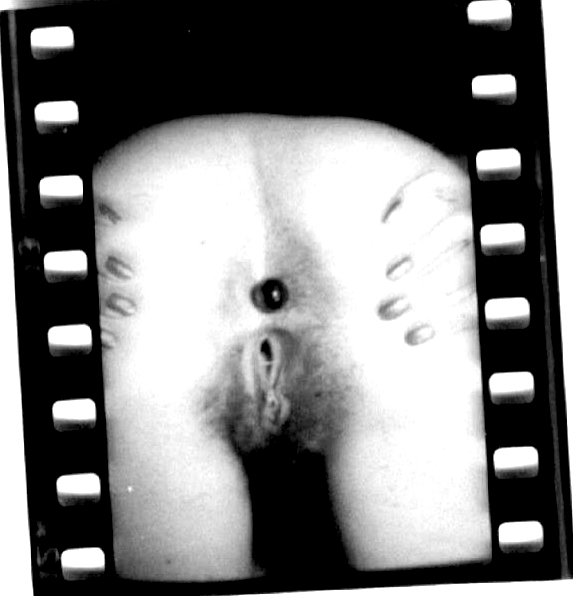
\includegraphics[width=9cm,height=10.6cm]{Imgs/img6.jpg}
\emph{Origem}, 1973
\end{center}

\section*{Vamos pôr um cu na vitrine\protect\footnote[*]{\MakeUppercase{F}rase
  atribuída a \MakeUppercase{D}écio \MakeUppercase{P}ignatari por \MakeUppercase{T}om \MakeUppercase{Z}é, em entrevista à \MakeUppercase{F}olha
  de \MakeUppercase{S}ão \MakeUppercase{P}aulo, sobre o projeto da capa de ``\MakeUppercase{T}odos os olhos'',
  de 1973. (\MakeUppercase{F}olha 2001)}}
\addcontentsline{toc}{section}{Vamos pôr um cu na vitrine}

\subsection{A história do olho}

Era 1972 e Tom Zé estava prestes a lançar o
\versal{LP} ``Todos os olhos'' pela Continental. Tom Zé encontra"-se com Décio
Pignatari, poeta à frente da agência \emph{E=mc²,} e pede"-lhe uma capa
provocativa, mas capaz de driblar a censura da ditadura militar
brasileira. Décio aceita o desafio e assim vem ao mundo a capa
internacionalmente conhecida em que um olho enorme parece imitado por
uma boca semicerrada no interior da qual era possível discernir algo
como uma gema de vidro. Mais de quarenta anos mais tarde, a genealogia
da capa permanece controversa e obscura, ainda que Tom Zé e, depois,
Chico Andrade tenham confirmado publicamente a suspeita de certos
olhares sobre a misteriosa capa do \versal{LP}.

Na ocasião do convite de Tom Zé, Décio sugere enfiar na capa um olho de
cu, mas que permanecesse irreconhecível como
tal.\footnote{``Colocaríamos uma bolinha de gude no
  cu e ampliaríamos esse cromo até começar a estourar os grãos da
  foto\ldots{} tornando a mesma irreconhecível a olho nu\ldots{}''.
  Em: ``A verdadeira (e única) história do disco do Tom Zé\ldots{}''. \emph{Blog do Chico Andrade}, 01/09/2012.}
No projeto\footnote{Tom Zé, em entrevista a Luiz Tatit
  e Arthur Nestrovski, narrou a origem da capa de ``Todos os olhos'':

  \versal{AN} - Podemos voltar ao Décio? Você não quer contar como foi
  a história da famosa capa {[}de Todos os olhos{]}?

  \versal{TZ} - Foi ele quem deu a idéia. Pensei que fosse desistir daquilo {[}a
  foto que aparece um olho, mas na verdade é uma bola de gude num
  ânus{]}, porque no princípio achei muito perigoso. Claro que a
  gravadora nunca poderia saber nada; a história só foi publicada por
  David Byrne na contracapa do disco The Best of Tom Zé.

  \versal{AN} - E de quem é o famoso ânus?

  \versal{TZ} - Ah, era uma modelo. Antes da bola de gude, que foi uma solução
  final. O Décio um dia me ligou, depois que eu já estava até
  esperançoso de ele ter se esquecido, ligou e disse assim: ``Tom Zé, já
  tenho algum material, o pessoal lá na agência fez algumas fotos.''
  Eram closes ainda não radicais, via"-se parte do bumbum da moça,
  parte das pernas, parte dos próprios órgãos genitais --- tudo muito
  acanhador para mim. Eu tinha que fazer o papel de civilizado, ``Muito
  bem\ldots{} Este ângulo aqui\ldots{} o enquadramento\ldots{} a luz\ldots{}'' Tudo mentira.
  Eu estava era com vergonha. Por fim, ele propôs a idéia de um close
  máximo. No fundo, acho que Décio tinha esse dilema: como botar isso na
  rua? Uma banda, naquele ano, tinha cantado num show a palavra
  ``seio'', e foi presa na descida do palco. Só pela palavra ``seio''\ldots{}

  \versal{LT} - Era outra época mesmo.

  \versal{TZ} - E esse cu ficou na praça da República! A gente ia lá visitar.
  Naquele tempo, realmente havia esse sentido de rebeldia, de dar um
  cascudo na visão militar do mundo e do Brasil, não é? A gente tinha um
  prazer imenso de ir lá e ver aquele cu na praça da República --- mas
  isso entre nós, aqui, muito famíia. (\versal{ZÉ} 2003: 229--230).}, o cu
seria mais um olho entre todos --- mas um olho tão corporal, tão
desconcertante e confuso, que muitos dos fãs de Tom Zé acreditaram por
longo tempo tratar"-se dos lábios de uma ex"-namorada de alguém que
sensualmente envolvia uma bola de gude.\footnote{Essa é
  a versão do fotógrafo Reinaldo de Moraes, a quem os créditos do miolo
  de ``Todos os olhos'' atribui a realização da fotografia de capa.
  Moraes contesta a versão mais conhecida, de Tom Zé e Chico Andrade.
  Segundo ele, nem a modelo era uma prostituta --- mas uma ex"-namorada
  sua, fã de Tom Zé e dos artistas da Tropicália~---, nem a foto que
  efetivamente se tornou a conhecida capa de ``Todos os olhos'' estampa
  um ânus, mas uma bola de gude envolvida pelos lábios de Vera.
  Empecilhos técnicos e o resultado final teriam impedido, segundo
  Reinaldo, que a fotografia da capa fosse a de um ânus (Cf. Athayde e
  Moares 2010).}
A versão mais conhecida é a de que uma modelo --- talvez uma ex"-namorada,
talvez uma prostituta, isso também é incerto~---, teria sido convidada
para posar para a capa. Segundo essa versão, nem o olho da capa era uma
boca, nem a boca imitava o olho vidrado da capa: o olho era, na verdade,
um cu abocanhando uma bola de gude. Importa muito pouco saber se se
tratava realmente de um olho, uma boca ou um cu, de uma ex"-namorada ou
de uma puta: a confusão imensa dos elementos, agora livres, do corpo se
oferecia como tal e sem qualquer predicado. Imagem pura que o olhar
captura, em 1973 o cu havia sido exposto na vitrine. Não se trata de
fazer jus a versão alguma, mas de dar o devido crédito à operação
impessoal e ontologicamente subversiva por detrás dessa confusão
infinita em que os objetos parciais paranoicos, obsessivos, histéricos e
perversos se permutam livremente. O que finalmente importa é compreender
como o agenciamento olho"-boca"-cu"-bola de gude da capa de ``Todos os
olhos'' funda uma filosofia dos corpos misturados e confronta o controle
repressor; como a metafísica pressuposta pelo sensível dessas imagens
reemerge, em sua diferença irredutível, na resistência black bloc.

\subsection{Todos os olhos se voltam para mim}

1973. O ano é o
mesmo do lançamento do álbum mascarado dos \emph{Secos \& Molhados}.
Enquanto o incógnito Ney Matogrosso desfazia seu rosto e oferecia seu
corpo frenético, um agenciamento entre o tropicalismo indomável de Tom
Zé e o concretismo obsceno de Décio e seus convivas usava um corpo que
se oferecia sem qualquer reserva --- com a generosidade dos namorados
apaixonados, mas também das putas --- para desterritorializar o olho (um
elemento de rostidade e captura) em proveito do corpo. Para saltar do
olho ao corpo, não bastaria o olho em máximo foco, ou os lábios
contraídos, envolvendo uma bolinha como um cu faria; só mesmo a total
indiferença entre uma boca e um cu abocanhando uma bola de gude para
contrafazer o rosto, do qual o olho pode ser metonímia, no corpo.

A provocação e o drible talvez quisessem expor a obscenidade da censura
e da ditadura no Brasil. Tom Zé e Décio queriam dizer, talvez
literalmente, ``o Brasil está um cu'' (Rodrigues 2007: 134). Porém, com
``Todos os olhos'', Tom Zé conseguira mais do que um jogo de
corpo; conseguira desterritorializar o olho para atestar sua pertença
última ao corpo. Já não bastavam os rostos mascarados e as
cabeças"-pesquisadoras --- oferecidas em uma bandeja, como na capa do
primeiro álbum dos \emph{Secos \& Molhados.} Era preciso curtocircuitar
dentro e fora, cabo e rabo, olho e boca, cu e gema. Na capa de ``Todos
os olhos'', Tom Zé e Décio convertiam o olho, protótipo biopolítico dos
insidiosos e universais aparelhos de controle e videovigilância,
princípio de aprisionamento do sensível, em mônada anal: em potência,
cada corpo envolve um mundo que é a um só tempo imagem sensível,
obscenidade e desejo. Primeira tese de uma filosofia dos corpos
misturados que ``Todos os olhos'' inventa: se é possível fazer
buraco"-negro com o corpo (olhos, boca, nariz, orelhas), só é possível
desfazer um buraco"-negro ao desterritorializar a rostidade na integral
do corpo. E isso se faz na superfície dos signos --- um olho que é uma
boca que é um cu --- que assinalam uma posição de desejo e um afeto que
percorre o corpo. O rubor ou o tesão que a obscenidade provoca são
afecções políticas porque atravessaram por um corpo, como matilhas sobre
um deserto.

A gema, superfície do olhar, encerra o protótipo de uma máquina
identitária que será pouco a pouco generalizada. A filosofia platônica
sempre sonhou o ``olho que se olha por dentro'' (Foucault 2006: 88--89),
como a alma que reconhece sua essência no \emph{Eidos} e desterra a
sensualidade, fonte do erro e do negativo. O ``conhece"-te a ti mesmo''
platônico é obra de um olhar interior, máquina identitária que
atravessará a história da filosofia até os cristãos assombrados em
sonhos pelo fantasma do próprio desejo. Janela da alma, o olhar atesta a
pertença do corpo a uma identidade prévia que circunscreve o corpo em
uma forma e aliena a ela suas potências. O olhar identitário, dobrado
sobre si, ou o olhar censor do estrangeiro que há em mim, prenuncia a
alienação da potência na forma em proveito de uma máquina identitária.

Se o olhar é o princípio do panoptismo que reduz a multidão confusa às
individualidades dóceis (Foucault 2012: 87--89; Platão 2011: 38--39),
nas sociedades de controle tudo se passa como se todos os olhos se
voltassem para mim. Qualquer possibilidade de ação livre no Brasil atual
encontra"-se sujeita ao controle dos aparelhos de captura de Estado e da
mídia que se sustentam indistintamente sobre uma dupla operação: captura
e registro; todos os olhos, mas também memória de inscrição infinita. As
sociedades de controle funcionam a partir de um princípio de inscrição e
registro disciplinar dos gestos. Esse princípio de inscrição e registro
disciplinar dos gestos assume a forma de uma memória dos menores
eventos, mas de uma memória tornada consciente, manipulável e
informacional. Mesmo as polícias têm se utilizado da vídeovigilância
pública e privada para reconstituir narrativas de crimes obscuros. Tudo
se passa como em um \emph{thriller }policial, em que as investigações
cravam as garras sobre o dorso quente de uma imensa memória que coincide
com a integral da realidade urbana. Como em um campo transcendental de
imagens --- como encontramos em Bergson (2001: 167--172) --- a imagem e os
acontecimentos que a envolvem dispensam toda forma de consciência. As
câmeras dos prédios de apartamentos, condomínios fechados,
estabelecimentos comerciais, controle de tráfego, coletivos e táxis,
viaturas policiais e ambulâncias, metrôs e estações de trem,
\emph{shopping centers}, estacionamentos e vias públicas são colocadas
lado a lado. As extremidades de seus cortes perceptivos formam um
gigantesco contínuo de captura e registro de imagens a que, por
princípio, nenhuma ação poderia escapar. Será, para sempre, possível
identificar sujeitos e atribuir autorias.

Do panoptismo de Jeremy Bentham à difusão dos aparatos técnicos de
controle social, a diferença é que o olhar virtual e sem registro das
disciplinas, senão pela consciência dos vigias, torna"-se agora o
controle atual insidioso que recobre todo o campo transcendental como
superfície de captação e como memória de inscrição e registro. Se o
cinema é a arte da recomposição do movimento através dos recortes e dos
quadros, o controle é o pesadelo de um cinema"-total: ele é a arte
governamental de tornar virtualmente contínuos os recortes e quadros
perceptivos a fim de capturar a totalidade dos movimentos. Sem produzir
nenhum percepto, nenhum afeto, ele repete nuamente toda a porção do
visível.

Tudo se passa como se a difusão imanente dos dispositivos de controle e
videovigilância imitasse o gesto bergsoniano que tentava provar a
existência de uma duração e de uma memória universais que penetravam o
real a partir da simultaneidade (Bergson 2006: 52--53). Trata"-se de
recobrir o mundo com consciências cujos recortes perceptivos toquem os
extremos uns dos outros e, por isso mesmo, tornem"-se capazes de
registrar simultaneamente os menores movimentos e as mínimas durações.
Trata"-se de capturar o fora (Lazzarato 2006: 69--73), mas também de
afirmar operativamente que não existe fora, de transformar o real em uma
platitude, de expropriar tecnicamente uma memória"-mundo que daria acesso
ao lado de fora.

Edward Snowden, talvez o preso político mais célebre do mundo hoje,
percebeu com predência a latitude dos procedimentos de controle
contemporâneos postos a serviço do combate ao
terrorismo.\footnote{Em uma carta aberta aos
  brasileiros, em que pede asilo político ao Estado brasileiro, o
  ex"-cidadão estadunidense e agora apátrida Edward Snowden afirma ter
  exibido provas de que ``Alguns governos estão montando
  um sistema de vigilância mundial para rastrear secretamente como
  vivemos, com quem conversamos e o que dizemos. {[}\ldots{}{]} essa
  vigilância ameaça tornar"-se o maior desafio aos direitos humanos de
  nossos tempos''. Em: ``Leia íntegra da carta de Snowden ao Brasil''. \emph{Folha de S.\,Paulo}, 17/12/2013.}
Os bancos de dados da \emph{National Security Agency, }nos Estados
Unidos, formam uma espécie de memória virtualmente integral dos menores
acontecimentos: pequenos débitos, recargas de celulares, telefonemas
interceptáveis, acessos a sites\footnote{Na
  mesma carta, Snowden afirma: ``Hoje, se você carrega um celular em São
  Paulo, a \versal{NSA} pode rastrear onde você se encontra, e o faz: ela faz
  isso 5 bilhões de vezes por dia com pessoas no mundo inteiro. Quando
  uma pessoa em Florianópolis visita um site na internet, a \versal{NSA} mantém
  um registro de quando isso aconteceu e do que você fez naquele site.
  Se uma mãe em Porto Alegre telefona a seu filho para lhe desejar sorte
  no vestibular, a \versal{NSA} pode guardar o registro da ligação por cinco anos
  ou mais tempo. A agência chega a guardar registros de quem tem um caso
  extraconjugal ou visita sites de pornografia, para o caso de
  precisarem sujar a reputação de seus alvos.''}.

Por trás desse aparato mnemônico virtualmente total, produz"-se uma
operação tão disciplinar quanto antropológica. A inscrição e o registro
das menores durações e dos eventos infinitesimais subordinam"-se a uma
lógica informacional que é, também, antropogênica. As menores memórias
de eventos cotidianos --- para as quais Snowden não cessou de chamar
nossa atenção --- constituem uma espécie de polícia da ação e do sentido
em escala planetária. As memórias"-informação não são senão seus efeitos
visíveis, palpáveis e manipuláveis que, atualmente, podem substituir boa
parte das investigações policiais. A vontade de saber, que a tortura da
polícia política no Brasil dos anos 60 e 70 praticava sem escrúpulos
tem, hoje, nesse imenso \emph{corpus }inscritor, sua fonte privilegiada.
As perguntas ainda são as mesmas, e vagam ao redor das identificações
espaço"-temporais e subjetivas: ``Quem?'', ``Com quem?'', ``Como?'',
``Quando?'', ``Onde?''.

Se uma memória"-informação manipulável é o produto extraído pelo aparato
técnico da máquina identitária, é na medida em que sua operação
específica supõe não apenas uma subjetivação do corpo a ser controlado,
mas, antes, a produção da própria memória que deve ser tornada
manipulável. A produção da memória"-informação, manejável pelas polícias
e mídias, sustenta"-se sobre uma memória"-arquivo, que se define pelas
operações de captura, inscrição e registro. Nem ``Todos os olhos''
bastariam sem a memória insidiosa de que o poder os dotou. Sob as
operações superficiais de uma memória"-arquivo, a polissemia de
\emph{archê} atesta a copertença entre memória arquivística, poder
nomológico e escritura da lei.\footnote{\emph{Archê} é
  a raiz grega que designa, ao mesmo tempo, ``o originário'', ``o
  primeiro'' ou ``o primitivo'', mas também ``o comando'' em sentido
  nomológico; sentido presente na palavra ``arconte'', que designava os
  magistrados encarregados de fazer as leis, ou de as fazer representar,
  mas também de interpretá"-las com exclusividade na antiguidade grega.
  No cruzamento entre o topológico (o lugar do depósito dos arquivos) e
  o nomológico (o comando que emergia da inscrição da lei no corpo no
  \emph{nómos}), encontraríamos o fundamento da autoridade (Derrida 2001: 12--13).}

Toda memória"-arquivo supõe uma antropologização da memória, que se torna
manipulável como uma lembrança consciente. Os aparatos de controle
realizam quatro operações ontológicas fundamentais:

\begin{enumerate}
\item Operação
metafísica: reduzir a memória"-mundo, e as potências de uma memória para
o porvir que os corpos podem atualizar, a uma memória antropológica;
dali para diante, toda memória será apreendida como reminiscência,
memória"-lembrança útil para uma consciência atenta aos perigos que o
instante presente encerra;
\item Operação nomológica: selecionar as
lembranças úteis aos poderes constituídos, eliminar as inúteis e
docilizar as perigosas;
\item Operação topológica: conservar arquivos que
encerram as inscrições e os registros da máquina identitária;
\item Operação arcôntica: monopolizar a produção e a interpretação dos
registros mnemônicos.
\end{enumerate}

Nada parece ser mais exemplar dessas quatro operações técnico"-políticas
dos aparelhos de controle do que as imagens espetacularizadas dos
confrontos entre black bloc e policiais, ou as imagens de suas ações
diretas contra símbolos do capital. Em um caso como em outro, os
registros dos eventos estão sempre subordinados à monotonia da narração
dos telejornais do horário nobre, codificados às margens de crítica
social que as mídias contrafazem e reproduzem no \emph{socius}. Se o
vandalismo black bloc primeiro assume uma forma de ascese \emph{contra o
rosto} liberadora do corpo em determinado horizonte político epocal, o
segundo vandalismo black bloc, que também decorre da destruição dos
rostos, é o vandalismo contra as operações ontológicas de controle.

Por definição, o black bloc é um anarquivismo. As mídias independentes e
as redes sociais visam a perverter as operações ontológicas dos
aparelhos estatais de captura, restabelecendo os direitos das
memórias"-mundo contra as memórias antropogênicas. As memórias"-mundo
equivalem a regiões inconscientes, ou não"-percebidas, do real (Bergson
2001: 284/158), mas também são indiciárias da persistência de uma
memória para o porvir que corpos podem estar em vias de atualizar em sua
ação. Se o corpo constitui o epicentro político por excelência, é porque
ele é um corte instantâneo nos devires das forças (Bergson 2001:
223/81). Se os poderes constituídos podem representar as forças
unificadas em um estado determinado, os corpos nos lembram a todo tempo
de que as forças só podem encontrar"-se em estado metaestável, em vias de
conjurar o estado em que são continuamente representadas. As ações
diretas black bloc contra os signos do ``capitalismo universal'' do
\emph{télos }histórico furam a seleção nomológica das lembranças úteis e
reinseminam o imaginário simbólico coletivo com os índices dos
potenciais da revolta que constitui a verdade mais superficial e, ao
mesmo tempo, profunda de qualquer revolução. As operações topológica e
arcôntica são desterritorializadas no \emph{corpus} da \emph{web} --- e é
impossível responsabilizar fenômenos fluidos e difusos quando o poder se
exerce mediante identificação de sujeitos ou grupos.

Ao reintroduzir a impureza política no seio do imaginário social ---
ainda que aparentemente sob a forma do negativo em que as mídias
significantes a convertem --- é toda uma memória para o porvir que pode
novamente infiltrar"-se por essa fissura imperceptível. A captura, a
inscrição e os blocos de significação que as mídias constroem no nível
da consciência coletiva não podem tratar a ação black bloc como um mero
indiferente político; a captura mesma já implica uma radical produção de
diferença política, ainda que apanhada pelo olho, quando deveria, como o
\emph{desejo}, ser apanhada pelo rabo.

O controle se caracteriza pelo entrelaçamento de múltiplas estratégias
de governamentalidade. A soberania, com o poder de vida e morte sob os
arcanos da segurança nacional, do combate ao terrorismo e da produção de
sujeições pelo terror do Leviatã; a disciplina, com a infinita topologia
dos corpos identificáveis, sua regulação moral operada no nível do gesto
e da virtualidade do gesto; a segurança, como o controle de todos os
olhos, de repente voltados para mim, mas que se espraiam em um campo
espaço"-temporal infinitamente aberto, constantemente indefinido e
insidioso. Se se pode afirmar, com Agamben ou Negri, que a exceção se
torna o paradigma de governo destinado a regular situações fluídas e
metaestáveis, é porque sua forma governamental permite articular
estrategicamente no controle as três dimensões fundamentais do poder e,
ainda, permite violar direitos humanos utilizando"-se da própria
gramática da defesa dos direitos humanos (Negri e Hardt 2006: 36 e
Douzinas 2007: 32--33). Eis o que Edward Snowden prova com o próprio
corpo, sob a dupla condição de testemunha (\emph{testis}) e sobrevivente
(\emph{superstes}), quando luta com todas as suas forças para se tornar
um apátrida e um refugiado, escapando à condição de preso político de
sua própria nação de origem. Arendt teria estado sempre certa ao afirmar
que o refugiado constituiria, após Auschwitz, a vanguarda de seu povo.
Não é possível determinar, ao certo, mesmo no caso de Snowden, se ``seu
povo'' se refere à população estadunidense ou aos refugiados
desnacionalizados em que os controles e as políticas que envolvem os
corpos de cada um de nós virtualmente nos converteram.

Seja como for, como na ontologia bergsoniana, em que as mais vastas
realidades materiais são circunscritas pela duração universal como
porções inconscientes do real, os dispositivos técnicos de controle
contemporâneos têm por objetivo expropriar essa memória"-mundo,
tornando"-a virtualmente manipulável e cronológica. Não se trata,
todavia, do mesmo tempo, nem da mesma memória ontológica elementar, que
Bergson interrogara, mas de análogos seus politicamente impotentes que
as tecnologias policiais fabricam: as capturas do fora equivalem à
expropriação dos mundos possíveis. Nas sociedades de controle, a memória
e as potências do tempo permanecem fechadas e virtualmente submetidas ao
campo perceptivo total que a arrogância dos controles descreve. Por
isso, hoje, a condição transcendental da ação livre, que entre os
antigos foram a ascese e a coragem parresiasta, tornou"-se a ação direta
das multidões sem"-rosto --- único modo de ação para escapar dos controles
insidiosos e criar um \emph{entretempo} no qual a ação política se
tornou, sob todos os olhares, novamente possível.

\section*{Olho por olho\protect\footnote[*]{\MakeUppercase{P}oema de \MakeUppercase{A}ugusto de
  \MakeUppercase{C}ampos, de 1964, que ilustrava, remodelado, a contracapa de ``\MakeUppercase{T}odos os
  olhos'' (1973).}}
\addcontentsline{toc}{section}{Olho por olho}

\begin{center}
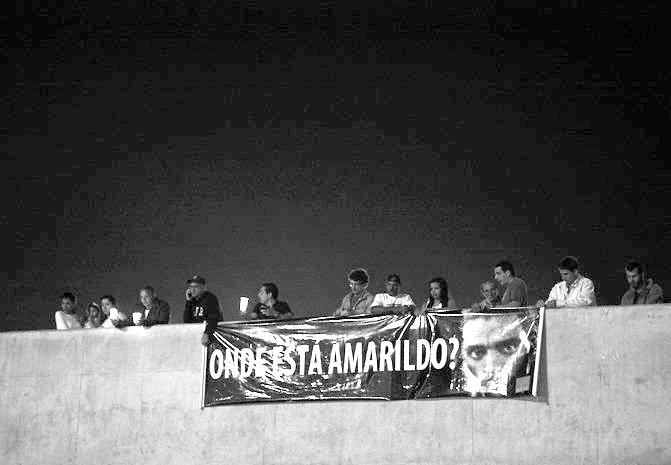
\includegraphics[width=9cm,height=6.1cm]{Imgs/img7.jpg}
\emph{Limite}, 2013
\end{center}

\subsection{Talião}

Em ``Todos os olhos'', o que nos olha é um olho
antiplatônico. Gema vítrea, borda confusa. Não se sabe muito bem onde
termina o olho e começa o corpo. Assim como foi preciso estourar os
macros da fotografia da capa do \versal{LP} de Tom Zé para ocultar o corpo como
sede material do olho, a ação black bloc precisa subtrair os rostos a
todos os olhos para liberar o corpo em um espaço controlado. O
vandalismo primeiro é uma espécie de ludismo contra a máquina
identitária. Olho por olho, entre o black bloc ou Tom Zé, não se trata
de conhecer a si mesmo, mas de deixar"-se afetar pelo real do corpo.
Expor o cu de uma \emph{jeune fille en fleur} em máximo foco na
vitrine não apenas testa o olho do poder, seus aparelhos de captura
simbólica, mas desafia a máquina repressiva com a mais sutil das
ameaças: o devir"-imperceptível. O imperceptível --- um pouco como
Deleuze, que enfiava as longas unhas no bolso do casaco --- é o signo
clandestino de toda revolta contra o platonismo identitário do poder.
Repetir o imperceptível, primeiro em si, contra o próprio rosto,
constitui um atentado contra a máquina identitária, o vandalismo
arqueológico.

Podemos nos ver na gema vítrea, mas jamais na borda confusa, que
assinala o corpo. O corpo não é espectral ou translúcido. Ele é a
muralha cerrada da alma, sua recusa ao mesmo tempo mais profunda e
profusa. De todos os olhos, o cu é o mais antiplatônico: a imanência
rósea do corpo, perversão da origem do mundo de Courbet. Enquanto
``todos os olhos se voltam para mim de lá de dentro da escuridão'', o
olho antiplatônico assinala o duplo fundamento da política: o corpo e o
desejo. Diferença profunda, simetria aparente: olho por olho\ldots{}

\subsection{Cademar(ildo) que não vem?}

Todos os olhos inscrevem e
registram os pequenos eventos, imagens dos corpos, dos seus movimentos,
remontagens infinitas, constroem mapas borgianos dos acontecimentos,
promovem capturas cronológicas, sustentam"-se em uma obscena máquina
identitária. Aquilo que um devir"-imperceptível revela é a copertença do
corpo ao desejo e do desejo ao corpo, ponto de partida da política. O
corpo só pode se tornar eficaz se puder ser tão clandestino quanto o
desejo, como uma rachadura que se propaga anônima em um prato (Deleuze e
Parnet 1998: 147). Sob todos os signos superficiais da revolta, há uma
emoção criadora que a precede --- como o poder constituinte é, ao mesmo
tempo, esteio e lado de fora do constituído.

Porém, a máquina identitária, positiva e fabril, sutil e disciplinar,
possui tanto um campo de atuação quanto um limite no corpo sobre o qual
se inscreve. Tanto se pode ``forjar uma alma'' como um efeito de poder
quanto aprisionar, torturar ou destruir um corpo. O limite de sua
captura é o desaparecimento material do corpo --- superfície física de
inscrição --- e a dimensão de sua prática não será menos biopolítica do
que a operação de forjar um rosto. O desaparecimento de um corpo pode
ser fabricado espiritualmente, pelo adestramento e pelas disciplinas,
como rearranjo das forças sediças, ou no nível da matéria, por sua
tortura e desaparição física. As prisões brasileiras estão a meio
caminho entre a produção da desaparição espiritual e a da desaparição
física. Também por isso, todo preso é um preso político; porque o
prisioneiro é, em primeiro lugar, o corpo --- posição de desejo que
coincide com a liberdade.

Sempre se trata de separar uma força daquilo que ela pode --- e o corpo é
a sede inconsciente das forças (Deleuze 2001: 65). Sempre se trata de
separar, portanto, em um corpo, suas forças do que elas podem. Como não
teria sido essa toda a estratégia profunda da história da filosofia
política no decorrer da modernidade ocidental? Na lógica da edificação
da cidade ideal, como na lógica soberana, trata"-se sempre de forcluir as
potências dos corpos, alienar sua multiplicidade na forma unitária do
corpo político. Assim como em Platão o poeta imitador instaurava na alma
do indivíduo um princípio de mau governo, lisonjeador da parte irascível
da alma humana,\footnote{``Se, porém, acolheres a Musa
  aprazível na lírica ou na epopeia, governarão a tua cidade o prazer e
  a dor, em lugar da lei e do princípio que a comunidade considere, em
  todas as circunstâncias, o melhor'' (Platão 2012: 469 {[}605a/606{]})}
em Thomas Hobbes os poderes inerentes ao corpo que descreviam seu
direito natural deveriam ser objeto de uma privação em comum a fim de
fundar uma comunidade política, renunciando ao seu direito sobre todas
as coisas ou transferindo"-o a um outro homem (Hobbes 2010: 72--73). Eis
como o corpo se torna o irrepresentável da política e, ao mesmo tempo, o
fundamento imperceptível e enigmático da soberania moderna.

Sob a célebre representação do Leviatã --- corpo soberano feito de
infinitos corpos --- já se pressente que a formação da cidade depende da
sujeição das multiplicidades dos corpos à forma do Um. Alienação da
potência na forma, ``submissão das vontades de todos à de um homem ou
conselho'' (Hobbes 2002: 96), o que significa redução da multiplicidade
dos desejos e apetites à vontade do Um, mas também cessão do direito de
usar as múltiplas riquezas e forças contra qualquer um; ``àquele que
submete sua vontade à vontade de outrem transfere a este último o
direito sobre sua força e faculdades'' (Hobbes 2002: 96), isto é, sobre
as forças de seu corpo. Hobbes dirá mais de uma vez que transferir a um
só homem ou a um conselho toda a sua força ``nada mais é do que abrir
mão do seu direito de resistência'' (Hobbes 2002: 98). Se o corpo é a
sede material das forças, ele é, por definição, o foco de toda potencial
resistência às forças que o penetram. Contra todas as ordens de afetos
políticos, os corpos individuais são organizados pelo afeto homogêneo da
ordem soberana. É o terror que o enorme corpo político inspira que
garante a concórdia e a unidade das vontades; terror, conjuração do
desejo.

Na lógica da soberania, o corpo resta elidido, a não ser como ponto de
aplicação do poder e sede de forclusão de seus potenciais específicos.
Os afetos perigosos que nutrem ou revelam as múltiplas composições de
forças que atravessam os corpos, que revelam sua resistência e liberdade
ontológicas contra a sujeição, permanecem inermes. Corpo e vida são a
direção ao mesmo tempo material e metafísica contra a qual a soberania
investe. Se Foucault (2009: 127--128) dissera que o velho direito de
soberania encontra na matabilidade seu fundamento primeiro, é na medida
em que ``fazer morrer'' significa anular permanentemente um corpo na
tessitura social das forças. A governamentalidade soberana é o desterro
do corpo para apropriar o corpo. Não apenas a vida, mas também o corpo
do vivo, são objeto de uma dupla exceção. Se a vida só ingressa na
esfera política na exata medida de sua intrínseca matabilidade --- como
quisera Agamben (2007: 90) --- um corpo, e as forças em um corpo, só
podem ingressar na esfera da soberania política na medida de sua
forclusão. O corpo designa a porção ingovernável de real que retorna nas
revoltas e as revela como tais. Toda revolta é sempre a revolta profunda
dos corpos, porque o corpo jamais se insere nos mecanismos de
representação política.

Mesmo como elemento de controle biométrico --- talvez a mais recente
máquina identitária que o Brasil tenha inventado --- o corpo entra na
política sem qualquer \emph{virtù; }assinalar sua identidade, ligar um
rosto a um corpo, a suas dobras físicas, revela o campo de inscrição do
poder, mas mantém ocultas as forças que um corpo conserva
irrepresentáveis. O corpo é, a um só tempo, matéria de sujeição e campo
incessante de subjetivação soberana. Em uma palavra, o corpo é
\emph{subject,} o sujeito político por excelência. Eis o que supõe a
construção de uma antropologia de fundo para os direitos humanos, cujo
advento teria assinalado que a vida se tornava, na passagem da soberania
régia para a dos Estados"-Nação, o portador imediato da soberania
(Agamben 1996: 134; Agamben 2007: 25).

Servindo"-se dele, seria preciso ir mais além de Agamben. O poder se
exerce sobre a vida dos corpos como forma para inscrever"-se no
\emph{corpus }da vida. Ainda que a vida seja a verdade profunda do
corpo, os corpos são a verdade mais superficial da vida, seu ponto de
encarnação e aparição, de construção de mundo, de sujeição e
resistência. Não há como produzir a exceção política da vida sem
forcluir o corpo, sem dominar suas forças, sem arrastá"-lo para fora da
política, sem sublimar sua multiplicidade de afetos no terror
virtualmente total que o Leviatã inspira e que sua polícia pratica. O
corpo é a base material sobre a qual todo poder se inscreve, faz memória
com ele, o espiritualiza --- como a tortura dos primitivos servia para
criar, no corpo, uma memória da lei (Nietzsche 2008: 50; Clastres 2003:
198--204). Princípio antrópico da genealogia da moral: o homem se torna
o animal capaz de fazer promessas apenas na medida em que o terror e a
crueldade forjaram, em seu corpo, uma memória e uma alma prenhes de
má"-consciência. Paradoxalmente, o corpo marcado assinala que a verdade
profunda do corpo é a alegria da crueldade --- seu sistema imanente de
afetos.

O corpo é, ao mesmo tempo, o Fora da política e a sua integral. Por essa
razão, de Platão a Hobbes, a cidade ideal só pode erigir"-se mediante a
forclusão de seus afetos, que são também suas forças e sua potência, as
intensidades que o atravessam de fora e as dobras com que um corpo cria
um lado ``de dentro''. É nesse sentido que o corpo desaparecido ou
oculto --- força separada da potência --- confunde"-se com o corpo ideal do
súdito. Dupla captura soberana: apropriação e, ao mesmo tempo, forclusão
do corpo pelo Um. Exclusão das potências do corpo --- sua multidão
indócil de \mbox{afetos~---,} invenção do corpo do súdito e construção do corpo
soberano. \emph{Reductio ad unum. }Mesmo que estejam de quatro, os
soberanos só sabem gritar ``Morte ao múltiplo!''.

Talvez por isso, a tortura e o desaparecimento sejam, ainda hoje, as
demonstrações mais bem"-acabadas da tese segundo a qual o corpo é, a um
só tempo, o fora e o fundamento da política. Durante a ditadura militar
brasileira, a repressão, a tortura e o assassinato sistemático de
opositores constituirão, ao longo de algumas décadas, os paradigmas de
exercício do controle social e da repressão estatais contra as
insurreições da luta armada revolucionária (Negri; Cocco, 2005: 103).
Mesmo após a transição ao regime democrático, esses aparatos
burocráticos não são desmontados, não sofrem purgas, tampouco são
reestruturados no Brasil. Pelo contrário, em pleno funcionamento, o
aparato de violência legal permanece atrelado às estruturas herdadas do
regime precedente --- o que poderia explicar, ao menos em parte, a
escalada da violência endêmica no Brasil e no resto do continente
latino"-americano pós"-ditatorial (Pinheiro, 2002: 240), especificamente
estruturada sobre o \emph{rapport }Estado"-cidadão que se desenvolve em
culturas políticas autoritárias marcadas pela violação a direitos
humanos e pela lógica da impunidade.

Vladimir Herzog está para o sistema de legalidade aparente da ditadura
militar brasileira como Amarildo de Souza está para a democracia
aparente do sistema de pacificação carioca. O ajudante de pedreiro é
ilegalmente preso para averiguação --- forma de prisão comumente exercida
pela polícia política da ditadura militar brasileira~---, é torturado na
sede da Unidade de Polícia Pacificadora da favela da Rocinha e
assassinado. Sua morte não é forjada --- como a de Herzog~---, mas seu
corpo é ocultado pelos policiais envolvidos. Três formas de anular um
corpo: prisão, tortura, desaparecimento. O fato de uma Unidade de
Polícia Pacificadora ter se tornado, ainda que temporariamente, sala de
tortura, revela a verdade profunda da pacificação como apropriação
política dos corpos. O assassinato de Amarildo e a ocultação de seu
cadáver torturado revelam, ainda, que do sistema de legalidade aparente
ao sistema legal de democracia aparente, o corpo jamais deixou de ser
fundamental para os regimes de governamentalidade. O paradigma de
governamentalidade das polícias militares --- como sua estrutura
constitucional --- não se alterou de 1967 para cá. Enquanto a sala de
tortura produz um corpo violado, e o assassinato político produz um
corpo sem vida, o desaparecimento produz a ausência de corpo (Teles 2010: 305) --- destino autofágico da soberania política moderna.

Amarildo, não o \emph{homo sacer}, é o corpo político paradigmático da
legalidade de democracia aparente do Brasil contemporâneo. O corpo de
Amarildo foi o laboratório total do poder constituído: corpo ilegalmente
aprisionado --- como o de Baiano ou Rafael~---, torturado e morto --- como
o de Herzog~---, e finalmente desaparecido. A faixa título de ``Todos os
olhos'' aparece como uma resposta, mas também como um produto do corpo
torturado. De vez em quando, vindos do fundo da escuridão, todos os
olhos interrogam um corpo, ``esperando e querendo que `eu' seja um
herói'', e que lhes responde: ``Eu sou inocente'', ``Eu não sei de
nada'', ``Eu sou até fraco''. Todavia, ``Cademar'' --- a canção que
antecede ``Todos os olhos'' --- expõe o corpo como o duplo e paradoxal
fundamento da polícia política de seu tempo. O corpo antecede e borda a
gema vítrea de todos os olhos saídos da escuridão; a desaparição do
corpo é, ao mesmo tempo, o fundamento material do exercício do poder e o
destino autofágico da política soberana. A tortura é a inscrição obscena
da lei no corpo. O desaparecimento, a clandestina e integral absorção do
corpo pela lei --- limite ideal das repúblicas.

Por isso, do Ato Institucional nº 5 a Amarildo, a terceira faixa de
``Todos os olhos'' nunca deixou de ser atual. Topologicamente, a canção
de Tom Zé antecipa a faixa que dá título ao \versal{LP} de 1973 sob a forma da
questão que invadiu as ruas em outubro de 2013. O ``Cadê Maria que não
vem?'', de Tom Zé, revela a genealogia temporalmente insistente das
desaparições políticas, hoje praticadas pelos grupos --- por vezes
policiais --- de extermínio, moralmente neutralizadas como ``guerra
justa'' contra o tráfico e o crime organizado (Negri; Hardt 2006: 34).
Entre 1968 e 2013, ``Cadê Maria?'' --- o grito poeticamente recortado e
politicamente abafado de Tom Zé em plena ditadura --- atravessou
insensivelmente por milhares de nomes, dos autos de resistência
injustificáveis aos enterros de corpos não"-identificados como
indigentes. Em outubro de 2013, os milhares de pequenos gritos
inaparentes e sufocados sofreram um efeito de acúmulo e ``Cadê
Amarildo?'' definiu"-se como a sua integral: integral dos mortos e
desaparecidos do sistema de democracia aparente do Estado brasileiro
pós"-1988.

As prisões arbitrárias de Rafael, Baiano e Amarildo constituem o signo
incontestável de que corpo e liberdade são a verdade profunda da
política --- verdade que deve ser dominada em suas forças profundas,
reduzida em sua multiplicidade ao Um, anulada em sua resistência
natural. Os corpos, a forclusão de seus afetos, sua tortura e
desaparecimento, são os limites da política e expõem a verdade profunda
da política e da lei que, não sendo pacificação, como quisera Hobbes,
são guerra (Foucault, 2002: 22--24 e 58--59) --- hipótese"-Nietzsche.
Porém, um filósofo mascarado já afirmara que o espírito não é uma cera
mole (Foucault, 2001: 927), mas uma substância reativa. Tampouco o
corpo é uma cera mole. Borda dissoluta, não sabemos o que pode um corpo.

Enquanto todos os olhos do controle espreitam o corpo, seu olho
antiplatônico imperceptivelmente exposto na vitrine espreita a
\emph{pólis. }Tornados irrepresentáveis pelo poder constituído, os
corpos multiplicam suas forças elididas; e as forças que espreitam a
\emph{pólis} são as mesmas que conspiram em silêncio, clandestinamente,
pelo tempo que for preciso --- até que uma ontologia profunda dos corpos
se encarne, inesperadamente, em uma fenomenologia da revolta.

\chapter{Beaglepolitik}

\begin{center}
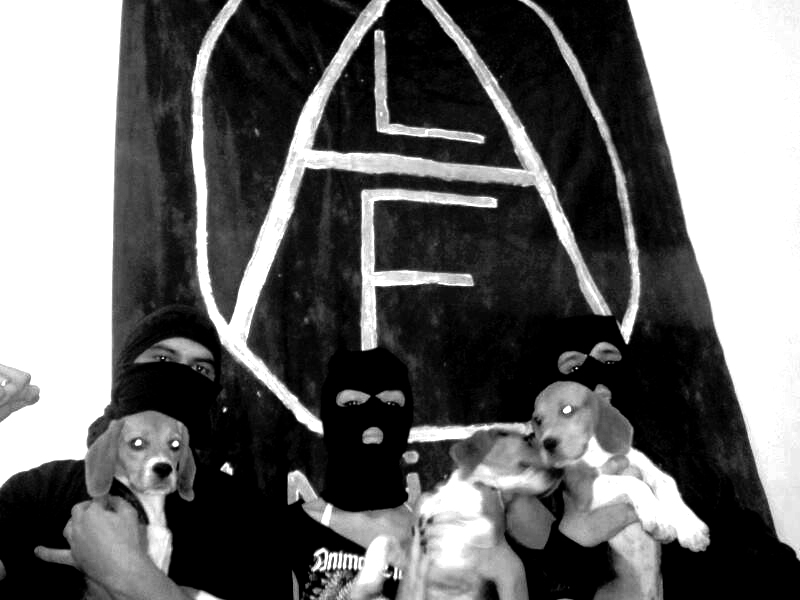
\includegraphics[width=9cm,height=6.1cm]{Imgs/img8.jpg}
\emph{Laboratório}, 2013
\end{center}

\section{O corpo é um bicho}

\textbf{}Quando Espinosa inscreveu no frontispício dos livros de
filosofia a questão ``\emph{o que pode um corpo?''}, queria dizer que
não sabemos \emph{o que é um corpo}. Enquanto toda a tradição metafísica
pré"-kantiana colocava em questão a demonstração de um Deus e de um
espírito transcendentes ao mundo, Espinosa era amaldiçoado por seu povo
por perguntar"-se o que constitui, em um corpo, o arranjo de suas forças
e sedições, das infinitesimais deposições de sujeições e subjetivações
que forjam, em um corpo, algo como uma alma inaparente e uma potência
divina de liberdade. Espinosa era amaldiçoado, ainda, por afirmar que a
mesma potência divina que era necessária a um ente para vir à
existência, era igualmente necessária para que ele perseverasse nela,
segundo seus modos singulares, suas paixões, desejos e apetites; e,
finalmente, por afirmar que a potência infinita de deus confundia"-se com
a potência da própria natureza: \emph{Deus sive Natura}. A imanência
espinosana trabalhava a quente contra a transcendência forjada a frio
pelos metafísicos.

Cada corpo age determinado por apetites e paixões, mais do que pela
razão e, por meio deles, cada um se esforça por perseverar na
existência. Sábios e tolos são igualmente partes da natureza e
esforçam"-se, segundo os modos singulares e afetivos de seu corpo, por
perseverar na existência. Em um caso como em outro, é a unívoca e divina
potência da natureza que atravessa os corpos e os determina a agir como
lhes convém --- segundo o desejo ou de acordo com a reta razão.

O corpo espinosano é um campo de variações de ações e paixões, e não há
potência para além dos afetos que o percorrem, como não há tristeza ou
alegria para além de um corpo. Responder à questão ``o que pode um
corpo?'' é, em Espinosa, perguntar"-se sobre os limites de sua potência,
o conteúdo variável de seu direito natural (Deleuze 1968: 236). Do
corpo, emerge um sistema imanente de direitos que coincide com os
conjuntos de potências e afetos definidos no campo de variação singular
que constitui um corpo. O direito de cada um estende"-se por definição
até o ponto em que se estende o seu desejo e a sua potência (Espinosa
2008: 234--235). Porém, quanto mais vivemos sob as injunções do terror e
do medo, menores são nossas capacidades de agir livremente, menor é
nossa compreensão sobre o desejo que nos habita. É preciso infundar toda
uma ordem hobbesiana e o terror pressuposto pelo \emph{rapport}
soberano"-súdito. É preciso relembrar as múltiplas escritas de um
anti"-Hobbes. Eis o ponto em que uma ontologia política reencontra a
verdade dos corpos, o desejo mais profundo que os corpos exprimem. O
corpo é o campo microfisiológico de rearticulação entre o erótico e o
político. O corpo é um bicho.

\subsection{Seu corpo vai se transformar num raio}

Tudo o que passa por um
corpo faz sua história mais ou menos demorada. Demografias, patologias,
processos metabólicos, necessidades e apetites, pestes, bacilos e vírus,
sujeição ao trabalho, conformação a cerimônias e a rituais. As
disciplinas transformam o corpo em um bicho de laboratório. Tanto quanto
a filosofia política da modernidade descobrira ser possível fabricar, no
corpo, um súdito de afetos anulados, o saber"-poder disciplinar e os
investimentos econômicos do capitalismo descobriram estratégias para
dobrar as forças de um corpo, a fim de transformá"-lo em corpo, ao mesmo
tempo, produtivo e submisso. A partir daí, um corpo é definido segundo
uma seleção estratégica de sua potência: corpo"-reprodução, corpo"-força
de trabalho, corpo"-produção, corpo"-usina. Porém, a seleção estratégica
deve significar, ao mesmo tempo, a adoção de estratégias microfísicas ---
exercidas no nível do detalhe, do gesto ou de seu esboço --- destinadas a
sujeitar certos vetores de forças que atravessam os corpos. Se as
estratégias disciplinares se definem pela fabricação de corpos dóceis e
úteis, é na medida em que as forças indóceis, de resistência e sedição
dos corpos, que os definem como tais, devem ser neutralizadas em
proveito da ação estratégica das disciplinas; alienação da potência na
forma de um arranjo fabril das forças de um corpo.

Eis o corpo político, objeto de investimento; objeto de violência e
ideologia, ponto de aplicação tanto da porrada quanto da propaganda mas,
principalmente, objeto de gestão estratégica, controle sutil e contínuo,
adestramento e laboratório fabril de produção de servidão voluntária (La
Boétie 1982). Nas disciplinas dos modernos, trata"-se muito mais de
investir um corpo de um conjunto de forças economicamente úteis e
politicamente dóceis do que de apropriar"-se dessas forças, como em um
pacto hobbesiano. Trata"-se muito mais de investir cada corpo como um
imenso laboratório das forças que de exigir sua rendição violenta. O
poder não é, portanto, uma coisa que alguém detenha, mas um nome que nos
acostumamos a atribuir ao ``efeito de conjunto'' das posições
estratégicas e para descrever os vetores ativos de dominação. A sujeição
voluntária de um corpo às disciplinas, como uma forma"-homem ou uma alma,
descreve antes os efeitos regulares dessa forma de exercício de poder do
que uma natureza naturada sempre já feita.

O poder tampouco implica obrigações ou interdições; seu modo de
exercício não é meramente repressivo ou violento: circulando entre os
corpos, por meio dos corpos, ele os investe e fabrica, apoia"-se neles
(Foucault 2012: 29). Portanto, seria um erro localizá"-lo pura e
simplesmente nos aparatos de Estado ou nas formas gerais da lei, se o
poder circula e se multiplica através dos corpos. Muito antes de ser a
propriedade de alguém --- do Estado ou de uma classe~---, o poder é algo
que se exerce em função de singularidades locais. Não pode, portanto,
ser descrito de maneira homogênea (Deleuze 1983: 33).

O ateísmo marxista venera o Estado analítica e estrategicamente, pois
crê encontrar na superestrutura a localização privilegiada do poder.
Porém, o Estado não pode constituir senão um efeito de conjunto de
posições estratégicas de uma microfísica que define as formas
metaestáveis pelas quais um poder circula pelos corpos, por seus pontos
estratégicos de submissão e singulares de sedição e revolta. Toda
revolução começa pela revolta que se produz, primeiro, nos corpos. Para
compreender adequadamente a natureza microfísica das mais infinitesimais
relações de poder, seria preciso abandonar uma teleologia da história em
proveito de uma ontologia política do devir; ainda, seria preciso
abandonar uma teoria da revolução redentora em proveito de uma práxis da
revolta que sempre esteve --- e ainda está --- nas ruas, mas jamais
ingressou nas bibliotecas.

Uma das principais teses de Foucault desde as primeiras páginas de
\emph{Vigiar e Punir} é a de que o poder não possui uma essência --- a
partir da qual seria possível atribuir aos sujeitos a qualificação de
dominantes ou dominados~---, mas o poder é operatório. Isto é, o poder
implica uma relação de poder; ele se define como um conjunto de relações
de forças que atravessam tanto pelos arranjos singulares que resultam em
forças dominadas como os que produzem forças dominantes. Mesmo o corpo
do submisso, do bicho de laboratório das disciplinas aplicadas ao corpo,
constitui ponto de apoio material para seu exercício. As forças não
podem produzir um tal arranjo se não circularem por ali, se não vencerem
as resistências que as potências indóceis de um corpo esboçam, se não
obliterarem as virtualidades mais ou menos espirituais que o percorrem.

Em uma entrevista concedida a Dreyfus e Rabinow, Foucault definira o
poder como relação da força com a força. Isso era uma forma de negar que
haja exercício de poder unidimensional, poder que se exerça simplesmente
como violência ou como ideologia, como porrada ou como propaganda. Há
sempre um ponto de apoio nos corpos que lhe corresponde, há sempre uma
imensa rede de contrapoderes e forças sediças a dominar e vencer, forças
das quais um corpo se deixa investir incessantemente e sempre em
relação. Nada de forças verticais e isoladas; mesmo a transcendência da
soberania se sustenta na horizontalidade aberta das microssujeições.

O corpo se determina, então, como um campo experimental das relações de
poder. O corpo se define, como uma perspectiva das relações de forças ---
borda dissoluta ou olho antiplatônico que todos os olhos do controle
vigiam. O corpo é um bicho de laboratório. Sempre se trata de definir
suas forças, conduzi"-las ao seu limite, experimentá"-las até o fundo de
suas resistências, dominá"-las, aplacar suas revoltas, torná"-lo
superficial. Toda relação de poder se define, então, como uma
anatomopolítica; a \emph{realpolitik }é uma \emph{beaglepolitik}.

\subsection{Teoria dos corpos anarquistas}

O corpo é uma perspectiva das
relações de força que se agenciam com ele. Contra todos os olhos, o olho
antiplatônico do corpo envolve e espreita o poder. Mas o corpo só pode
ser uma perspectiva das relações de força porque tais relações circulam
pelos corpos das multidões confusas, encontram nos corpos seus pontos de
articulação e apoio, agenciam"-se com eles, combatem estrategicamente
suas resistências. Assim como o poder explode contra as multidões nas
ações criminosas legalizadas pelas formas jurídicas do Estado e do
capital"-dinheiro, os corpos misturados explodem, também, a partir delas.

Toda ação black bloc se define como a criação de um entretempo em
que a política se tornou novamente possível. Sem identidade ou controle,
sem rosto e sob nenhum olhar senão o do olho antiplatônico --- que é puro
corpo~---, a condição de possibilidade da ação política investe"-se
plenamente nos corpos e na multiplicação dos corpos, na suspensão das
disciplinas e na reemergência de suas potências forcluídas. Como em
Espinosa o vir à existência de um ente e seu desejo de perseverar na
própria existência demandavam a mesma potência eterna da natureza,
resistência e reexistência coincidem nos corpos irredutíveis que compõem
os blocos negros. As multidões efetuaram a passagem das redes às ruas,
do cérebro eletrônico, de Gilberto Gil, à práxis concreta de uma
filosofia política dos corpos misturados.

Sob o eu social --- superfície verminal construída por mil e uma
microssujeições (como viajar em ônibus lotados, pagar mais do que um
serviço público vale, dar"-se conta dos lucros astronômicos dos
empresários do setor de transportes, conhecer as grandes ilegalidades
convalidadas pela lei que torna essas malhas de poder cada vez mais
tesas e ``naturais''\ldots{}) --- não cessam de se acumular e renovar as
potências rebeldes, os contrapoderes de corpos indisciplinados, indóceis
e, do ponto de vista dos poderes que se organizam para sujeitá"-los,
inúteis.

Na medida em que, contra o Estado, produz"-se a revolta profunda de todos
os corpos, esses corpos convertem sua fenomenologia da revolta em uma
ontologia da liberdade. Descobrem que a única consistência da liberdade
é a práxis da rebelião e, ao mesmo tempo, que a única forma de fazer uma
rebelião que seja também uma festa de destruição de todos os valores
contestados é tomando parte nessa experiência de liberdade. Sob a práxis
está a descoberta revolucionária de todos os corpos indisciplinados:
\emph{jamais fomos sujeitos}! O poder que circula pelos corpos --- seus
fluxos domados e axiomatizados pelo capital, pelo Estado, pelos aparatos
micrológicos e microfascistas das sociedades de controle --- é desejo
\emph{esquizo}, potência revolucionária. Rebelando"-se contra as
disciplinas, todos os corpos poderão, um dia, descobrir"-se profundamente
anarquistas, questionando a repartição do lícito e do ilícito a partir
das ações \emph{borderlines }como a de quebrar vidraças de bancos ou
depredar estabelecimentos capitalistas, usar máscaras, incendiar lixo ou
pichar palavras de ordem --- travar discursivamente, também, esse combate
pela produção de signos e pelo sentido comum do sensível (Rancière
1996).

O anarquismo profundo dos corpos confunde"-se com a descoberta prática e
concreta de que os corpos não são apenas feitos de investimentos do
poder, mas podem ser o laboratório ascético ou coletivo de
desarticulações que revelam, no corpo, a insistência de poderes sem
investimentos. Não basta rasurar o \emph{cogito. }Mais do que uma
política, desfazer o rosto tornou"-se condição da política; mas ainda é
preciso tornar o corpo impessoal a ponto de não mais reconhecer a
extensão que cotidianamente vemos refletida no espelho. Vestir"-se de
preto, mas jamais ceder a potência de seu corpo ao Estado ou a
grupelhos; tornar o corpo impessoal para liberá"-lo como uma força, uma
potência específica ou um raio. Podemos não sabê"-lo, mas se trata de
jamais renunciar àquilo que um corpo pode. Por isso, black blocs não
podem se confundir com sujeitos, grupos ou organizações, mas encarnam as
ações impessoais, praticam uma política do impessoal. Podendo ser algo
aquém ou além de um homem, a ação black bloc dissolve as cisões entre
homem e animal para revelar a sombra do animal contemporâneo ao homem;
ou, para revelar o homem como um animal biopolítico e seu corpo como um
bicho de laboratório. Não basta liberar o homem, que é um efeito de
poder. É preciso liberar o corpo, pois o corpo nos encarrega de nossos
animais. Encarregar"-se de nossos animais é atestar, mesmo que de um modo
obscuro à representação ou à inteligência, a copresença do primitivo.

\subsection{Queremos guerra}

``A guerra é a relação social fundamental''.
Escritores tão heterogêneos como Foucault e Clastres, sobre substratos
tão díspares quanto a formação das sociedades soberanas ou a lógica
guerreira nas sociedades primitivas, puderam afirmá"-lo. ``O natural, ou
o primitivo, persistem sob as infinitas camadas de cultura''. Tese de
\emph{As Duas Fontes da Moral e da Religião}, de Henri Bergson, mas também
do Manifesto Antropófago oswaldiano. Do entrecruzamento das duas teses,
o desejo de múltiplo que os corpos black blocs exprimem agencia"-se em
uma revolta contra o Um, em que a ação direta --- o vandalismo contra
bancos, caixas eletrônicos e empresas"-símbolo do capitalismo industrial
avançado --- é criador de um sentido a um só tempo novo e primitivamente
iniludível, contra as divisões sociais duras e segmentares que as
sociedades com Estado impuseram. Sob as infinitas camadas de cultura,
afirmar que o primitivo existe é, de algum modo, reafirmar que os corpos
não cessam de insistir e reexistir também ali.

O corpo é o primitivo, o aborígene e o nômade das estepes que jamais
deixou de ser --- apenas deixou de ser atual, ou ativo. Se a política
moderna forclui certas potências dos corpos a fim de investir outras,
dóceis e úteis, a persistência do primitivo encontra nas forças
indóceis, inúteis e revoltosas dos corpos seu princípio contra o Um.
Seria preciso falar, antes, nas multiplicidades e nas singularidades dos
corpos; no singular, ``o corpo'' não passa da grade de análise que
utilizamos como metáfora unívoca das multidões.

Clastres escrevera que uma linha divisória atravessa a história das
sociedades e as reparte entre sociedades com e sem Estado, sociedades
marcadas pela divisão entre dominantes e dominados e sociedades
indivisas ou, para utilizar torpemente um mitema ocidental, tais
divisões correspondem às sociedades selvagens e civilizadas. A etnologia
de seu tempo insistia em ver nas últimas uma forma evoluída das
primeiras, enquanto Clastres queria demonstrar sua diferença de natureza
irredutível. Jamais teria sido estruturalmente possível gerar Estado no
seio de sociedades primitivas --- não por uma falta de desenvolvimento
destas, mas por razões de ordem estrutural, de operações que conjuravam
a cisão interna do poder no corpo social, como a chefia e a guerra.

A modernidade eurocêntrica quase sempre sonhou as sociedades primitivas
como a matéria perdida que daria consistência ao hipotético estado
pré"-social que, por desenvolvimento, progressão ou contrato, estaria na
origem da gênese do Estado, da genealogia profunda da divisão entre
dominadores e dominados, que julgavam ser, desde Platão ou Aristóteles,
politicamente constitutiva. A hostilidade natural dos índios
comprovaria, finalmente, a tese hobbesiana de que a guerra de todos
contra todos termina por dar origem ao Estado e estruturar as divisões
políticas em que ele se sustenta.

Se Foucault (2002: 59) identifica o limite do pensamento político
moderno na inversão da fórmula de Clausewitz --- ``a política é a guerra
continuada por outros meios''~---, mostrando que a lei, nascida em meio
ao sangue e à lama das batalhas, não é pacificação, mas signo real da
dominação dos vitoriosos sobre os vencidos, Clastres descobre na máquina
de guerra primitiva uma relação social fundamental de outra ordem, que
sustenta a aliança e a troca, que é uma operação do \emph{nómos }próprio
às sociedades primitivas, que se inscrevia nos corpos dos jovens durante
os rituais iniciáticos. As sociedades primitivas jamais foram sociedades
sem Estado, mas sociedades \emph{contra }o Estado, que conjuravam a
formação de um órgão de poder separado do corpo social (Clastres 2011:
138). O lugar real do poder, e do desejo de poder, nas sociedades contra
o Estado, é o corpo social ``que o detém e o exerce como unidade
indivisa'' (Clastres 2011: 142).

Com isso, Clastres infirmava a tese da pretensão trans"-histórica da
existência do Estado e produzia uma fissura incolmatável na linearidade
simples dos modernos que acreditavam ter encontrado entre os selvagens o
\emph{missing"-link}: ``o Estado não é eterno'', ``ele tem data de
nascimento''. Depois de Clastres, não se poderia mais colocar a questão
da gênese do Estado da forma que ela se insinuava entre os modernos.

Sob a etnofilosofia selvagem de Clastres se dissimulava uma tese
profunda sobre a natureza formal do poder, cuja pressuposição se poderia
descobrir em uma linha divergente da filosofia política europeia
inaugurada por La Boétie: ``a divisão {[}entre dominantes e dominados{]}
não é uma estrutura ontológica da sociedade'' (Clastres 2011: 150). Por
mais que tenhamos perdido a lembrança de sua existência, a sua
desmemória é insistente. Claro que não podemos nos iludir sobre retornos
--- nem La Boétie, nem Clastres, ou Deleuze, o faziam. Porém, insistem
nos corpos civilizados vetores políticos de forças selvagens que é
preciso estimar. O primitivo é o imemorial contemporâneo --- tese
bergsoniano"-oswaldiana.

Clastres (2011: 217) não cessará de afirmar que o ser social das
sociedades primitivas é um \emph{ser"-para"-a"-guerra}. Deleuze e Guattari
(2007: 22) perceberam que a ``a organização da máquina de guerra é
dirigida contra a forma"-Estado, atual ou virtual''. Exterior ao Estado,
a máquina de guerra é o princípio operatório do contra o Um. A guerra
conjura a gênese efetiva ou potencial do Estado. Trata"-se de evitar o
mau encontro, de evitar toda corrupção do desejo de prestígio (comum ao
chefe como ao guerreiro) em desejo de poder. Trata"-se, sempre, de
abandonar quem ``quer bancar o chefe'' ao desprezo e à morte.

Porém, o que significa conjurar pela guerra a forma"-Estado? O que é o
``contra o Um''? O Um determina o nascimento de um polo de poder
separado do corpo social, transcendente em relação a ele. O nascimento
da forma"-Estado --- que Deleuze e Guattari (2007: 21) dizem ser um
``golpe de gênio'', não uma evolução, um desenvolvimento das forças
produtivas, ou uma diferenciação das forças políticas --- pressupõe
divisão, cisão e hierarquia; em uma palavra: distinção entre governantes
e governados. A guerra trata de evitar o infortúnio e o mau encontro,
consiste em um modo de existência que afirma a igualdade de cada um no
seio social, de uma maneira de perseverar em seu ser indiviso. Conjurar
a forma"-Estado, guerrear contra o Um, manifesta um irredutível desejo de
multiplicidade e diferença na manutenção de uma intranscendência social
do poder. Os poderes não podem fugir aos corpos, pontos de fusão e
multiplicação dos corpos anarquistas nas multidões confusas. \emph{Nómos
}contra a \emph{lei, }as multidões de singularidades insistem em uma
forma de diferenciação contínua que não implica divisão interna ou
hierarquia, que resiste a separar os poderes dos corpos em uma unidade
política distinta.

Por isso, conjurar a forma"-Estado é muito mais do que uma operação
negativa que visa a destruir uma formação política em estado nascente.
Ela só pode aparecer assim aos olhos de espíritos civilizados. A
exterioridade da máquina de guerra nas sociedades primitivas era
construída em um sentido absolutamente positivo, que era o de manter o
poder em uma relação imanente com o corpo social; combater, com a
máquina de guerra, toda e qualquer formação de poder separada ou isolada
do corpo social. Bastava ignorar as palavras do chefe, rir delas ou
abandoná"-lo à morte para garantir a imanentização da chefia aos
agenciamentos coletivos de desejo; bastava subordinar a guerra aos
interesses da coletividade, como todo indiviso, fazendo do guerreiro, de
sua capacidade técnica e de seu desejo de prestígio um simples
instrumento a serviço do corpo social indiviso; bastava converter as
corrupções do desejo de prestígio em desejo de poder em
ser"-para"-a"-morte, o que impedia pragmaticamente o aparecimento de uma
classe militar dirigente; finalmente, bastava conceber a guerra como uma
forma de indisciplina fundamental.

O ser contra o Um das sociedades primitivas é apenas o enunciado
civilizado, assombrado pelo negativo, que oculta o desejo profundamente
positivo de multiplicar o múltiplo (Clastres 2011: 248), de jamais
alienar o poder que percorre os corpos das multidões confusas a uma
forma"-Estado separada dele. Afirmar que a guerra é uma máquina exterior
ao Estado e à sua conversão em aparelhos militares significa
subordiná"-la a uma forma positiva de desejo que se entranha e reparte no
corpo social, que impede a sacralização da violência nas instituições
estatais ao mesmo tempo em que atesta a copertença entre poder e sua
imanência à multidão de corpos penetrados por uma indisciplina
fundamental.

Talvez por isso, em \emph{Queremos Guerra} --- a última faixa de
\emph{Gilberto Gil}, de 1969, escrita por Jorge Ben Jor --- a guerra
aparecia como um grito imenso, mas subordinado ora à mobilidade da
paixão e do desejo (``mas só se não fizer sol amanhã''), ora à
hostilidade e ao gozo ridículo (``Mas só se for para brigar / com a
minha sogra''). Ao mesmo tempo, a guerra é efêmera (``A guerra é um só
momento'') e constitui o sustentáculo imemorial (``Depois da guerra, /
Vem o esquecimento'') das alianças (que ensinam ``Como é feia a guerra /
Como é lindo o amor''). Mais do que gerar um ente político separado que
viria contê"-la --- um Estado hobbesiano contra a guerra~---, a guerra ou o
genocídio constituem função da forma"-Estado em sua gestão necropolítica,
de modo que \emph{viver é ingressar em uma guerra permanente contra o
Estado.}

A máquina de guerra parece funcionar por toda a parte em que há corpos
investidos de poderes, cedendo ou resistindo a eles, formando
blocos"-sujeitos ou blocos"-negros de corpos insubmissos ou liberados.
Trata"-se sempre da mesma máquina selvagem operando por baixo das
estruturas do Estado e, até mesmo, parcialmente capturada por seus
aparelhos militares e convertidas em máquinas de morte e abolição. Por
toda parte em que se faz ouvir uma máquina de guerra, \emph{isso
}funciona: a máscara contra o rosto, olho antiplatônico contra o
controle, vandalismo contra a propriedade, a sociedade contra o Estado.
Assim como a dissimulação do rosto é a recusa de um rosto biopolítico
que o poder inventou para cada cabeça, a dissimulação dos corpos
envoltos em vestes negras é o índice de uma operação ontológico"-política
em profundidade: a destruição de um corpo biopolítico e disciplinado, a
liberação de forças indomáveis e selvagens que se redescobriram na
multiplicidade confusa dos corpos. Sua aparente homogeneidade não
designa a forma interiorizada de um grupo identificável. Sugere, antes,
o pressentimento de uma sociedade indivisa que está no devir ou no
ecúmeno das sociedades divididas. Desejo de multiplicar o múltiplo, de
conservar a imanência de suas forças aos corpos das multidões prenhes de
singularidades confusas e potências inaudíveis.

\begin{center}
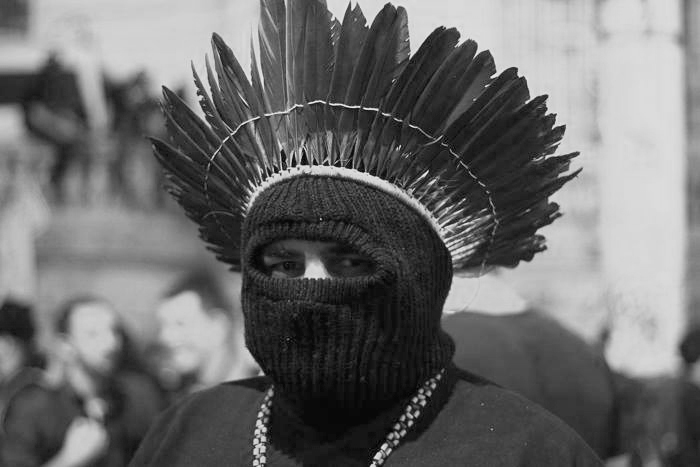
\includegraphics[width=9cm,height=6.1cm]{Imgs/img9.jpg}
\emph{Um índio}, 2013
\end{center}

\section{O homem é o fuleco do homem}

Até a metade dos anos cinquenta, a canção popular brasileira foi
espiritual, uma expressão sentimental. Nada, ali, se parecia com um
corpo. Muito romantismo, mas nenhum erotismo. Muito Apolo, mas nenhum
Dioniso. Muita beleza clara, mas nenhuma obscura embriaguez. A voz
sublime dos cantores da era do rádio formava um código expressivo e, ao
mesmo tempo, uma metonímia total da canção. O tropicalismo, porém,
reinventava a dimensão ritual da música (Favaretto 2007: 35) e
reintroduzia o corpo na canção. Em 1969, Gilberto Gil gravava pela
Philips um \versal{LP} que levava apenas seu nome, mas ficou conhecido como
``Cérebro Eletrônico'', especialmente após uma regravação da canção que
abria o álbum em 1996, por Marisa Monte. Assim como os corpos black bloc
se vestem de preto para produzir a reinserção do corpo na política,
Caetano Veloso, inspirado por Hélio Oiticica, vai vestir"-se de boá rosa
ou com roupas de plástico a fim de restaurar a dimensão profundamente
ritual do corpo erótico na música. Seu ponto de chegada e integração é o
corpo"-\emph{performance} dos \emph{Secos \& Molhados}, a expressão
integral das bordas dissolutas do corpo. A Tropicália fez da cultura a
sua natureza própria e íntima. O corpo, o campo ritual de fusão e
indistinção das cisões entre natureza e cultura.

 

\subsection{Tática}

Se os poderes que investem os corpos se definem
mais por sua distribuição imanente do que por sua unificação em uma
esfera separada, é preciso interpretar a ação direta black bloc para
além de toda significação negativa. É comum que as ações diretas sejam
definidas em função de uma tática simbolizada como ação sem sentido,
signo de niilismo político. Sob essa interpretação, as ações diretas
tornam"-se reféns do negativo puro ou de suas reduções simbólicas. O
ponto em que a tese da persistência do primitivo encontra a tese da
guerra como relação social fundamental, especialmente entre os
primitivos, não poderia ser outro: nos corpos, nos afetos e poderes
ontologicamente inseparáveis deles, insistem as virtualidades de uma
máquina de guerra que sempre pode ser inventada --- como uma malta contra
o Império. Portanto, é sob condições históricas irredutivelmente
heterogêneas que o black bloc tem em comum com as sociedades primitivas
a capacidade de invenção de uma máquina de guerra contra o Um. Eis o que
torna necessário perspectivar sua tática do ponto de vista de sua
positividade interna. Nada, na articulação concreta entre máquina de
guerra e persistência do natural, se assemelha a um anarco"-primitivismo;
já afirmamos mais de uma vez que retornos puros não são
possíveis.\footnote{``Homens de guerra
  renascem, com muitas ambiguidades; são todos aqueles que sabem da
  inutilidade da violência, mas que estão na adjacência de uma máquina
  de guerra a ser recriada, de revide ativo e revolucionário. {[}\ldots{}{]}
  Eles não ressuscitam velhos mitos ou figuras arcaicas, são a nova
  figura de um agenciamento trans"-histórico (nem histórico, nem eterno,
  mas intempestivo)'' (Deleuze e Guattari 2007: 84).}

Assim como Clastres pretendeu escrever o anti"-Hobbes primitivo, seria
preciso ensaiar uma espécie de anti"-Hobbes black bloc como a invenção de
um modo concreto contemporâneo de conjuração do infortúnio e do mau
encontro. Por meio dele, trata"-se de efetuar um largo salto da tática,
interpretada como ação sem sentido, à tática como horizonte de
instauração positiva de sentidos e de sua multiplicação.

Se a máquina de guerra permanece externa em relação ao Estado, a tática
será um conceito irredutível ao vocabulário militar. Ela está mais
próxima dos afetos que definem as linhas de latitude e longitude pelas
quais operam no cerne dos corpos; as táticas operam sempre como
descargas emocionais rápidas, projéteis velozes, como horizontes de
mobilidades contínuas (Deleuze e Guattari 2007: 79). Assim como a
tática é sempre a tática dos corpos que operam por afetos, os afetos são
como suas armas. Se perguntarmos a qualquer não"-policial e
não"-jornalista como nascem os quebra"-quebras em meio às manifestações,
obteremos a reposta: ``contra a violência policial''; se perguntarmos a
qualquer não"-policial ou não"-jornalista sobre a gênese da violência
black bloc, descobriremos que ``o Choque começou a bater sem qualquer
motivo''. A máquina de guerra é uma das respostas práticas sobre a
questão espinosana: ``o que pode um corpo?''. A tática não passa de uma
linha de desenvolvimento, ou de efetuação, de seus potenciais afetivos e
de ação.

O black bloc define"-se como uma tática, isto é, como uma multiplicidade
virtual de afetos que só podem definir"-se em concreto e em função de
corpos que perderam qualquer qualidade subjetiva: sem rosto e imunes aos
olhares, mas também contra o corpo das disciplinas, as roupas negras
ajudam a fabricar um corpo ritual e intensivo, cujas ações diretas
remetem a imensas constelações de ações livres (Deleuze e Guattari 2007: 79). As ações são corporais, mas tornaram"-se, ao menos na duração
intempestiva de um entretempo, inimputáveis a qualquer sujeito. Por
isso, é ingênuo esperar que as ações diretas não contrastem com
ordenamentos jurídicos positivos constituídos; mais profundamente, elas
colocam em xeque os próprios parâmetros de qualquer sistema jurídico ---
eis um de seus principais sentidos inaugurais, expor a fratura entre o
sistema legal de democracia aparente e os ilegalismos sobre os quais tal
sistema é constituído (dos bancos às empreiteiras, dos megaeventos às
remoções, dos lucros astronômicos à reprodução social da miséria e da
fome naturalizadas). Tudo se passa como se a integralidade de um sistema
jurídico unitário pudesse ser colocada em xeque por uma ordem jurídica
do múltiplo em que os corpos, indisciplinados e anarquistas, inventores
de uma multiplicidade nova de forças operativas --- uma máquina de guerra
contra o Um e o monismo jurídico estatal --- afirmassem seus ``direitos
naturais'', que coincidem com aquilo que seus corpos podem.

Sem suspender o ordenamento jurídico vigente, sob o risco constante da
identificação, do processo e da condenação pelas mais derrisórias
atitudes --- como vestir preto, dissimular o rosto, ``portar''
desinfetante ou vinagre~---, tudo se resume em contestar abertamente a
repartição entre legalismos e ilegalismos que constitui um ordenamento
jurídico. Tudo funciona como uma filosofia do direito dos corpos
misturados contra toda a teoria jurídica de Estado. Ainda que efêmera,
práxis de pluralismo jurídico, explosão das potências elididas do corpo
em direitos absolutos contra o poder que as subjugam.

A tática é a expressão prática do ``todos contra o Um'': ela revela a
insistência de direitos no \emph{fora} do sistema jurídico legal (as
potências elididas dos corpos), contesta a sacralização da violência no
monopólio coercitivo do Estado, de suas instituições policiais e
militares (pela ação direta dos corpos), instaura um potencial de
ruptura, a partir da ação, contra um sistema de legalidade que é
abolido, ou suspenso, assim que seus arcanos se encontram de algum modo
confrontados. Sob todos os sentidos, a tática --- armas dos corpos,
afetos de uma máquina de guerra --- é um contradispositivo (Agamben 2009: 42--51). Sua práxis produz uma reatriculação, ainda que singular,
intempestiva e efêmera, entre corpos e poder, ontologia e política. A
reinserção do corpo na política é uma espécie de tropicália black bloc:
anula o \emph{homo} em proveito do bicho --- que nem se confunde com um
animal, tampouco deve ser antropomorfizado.

\subsection{Dois eventos proliferantes}

Em certa noite da primeira semana
de outubro de 2010, na cidade Porto Alegre, um imenso mascote inflável
com a forma de um tatu"-bola colorido --- ``garoto"-propaganda'' de uma
marca de refrigerantes global que patrocinava a Copa do Mundo da \versal{FIFA},
no Brasil --- é atacado por manifestantes contrários à realização do
megaevento. Esse teria sido o ato final e ironicamente trágico da
manifestação, que foi acompanhada e, finalmente, reprimida pela tropa de
Choque da Polícia Militar do Estado do Rio Grande do Sul. Algumas horas
mais tarde, um jornal local estampava uma manchete em seu \emph{site}:
``Porto Alegre: Fuleco é esfaqueado por manifestantes''. Após o
incidente --- a imolação ritual de um ídolo do capital~---, as polícias
municipal e estadual reforçaram o esquema de segurança da mascote da
Copa do Mundo.

Na madrugada do dia 17 de outubro de 2013, na cidade de São Roque,
ativistas de diversas organizações civis pró"-liberação animal e black
blocs renderam os seguranças e invadiram a sede de uma empresa
farmacêutica que utilizava animais para realizar testes de seus
produtos. Sua ação libertou mais de duzentos cães da raça beagle,
que supostamente estariam sofrendo maus"-tratos. Em novembro do mesmo
ano, os ativistas retornaram à sede da empresa e libertaram centenas de
camundongos que, supostamente utilizados como cobaias, também teriam
sofrido maus"-tratos.

Fuleco esfaqueado e os beagles resgatados. Dois eventos
proliferantes na medida em que revelam cisões antropolíticas inaparentes
na cultura política ocidental, ao mesmo tempo em que sugerem um
potencial de abertura das ações diretas black bloc na direção precisa de
uma ontologia política do corpo que ultrapassa, em ambos os sentidos, a
forma ocidental de pensá"-la: nem animal, nem humano, o corpo é um bicho.

A cada evento corresponde uma perspectiva. Sob a figura murcha de
``Fuleco esfaqueado'' --- resultado de sua imolação quase"-ritual ---
oculta"-se uma verdade meta"-histórica da política no Ocidente que, de
Aristóteles a Hobbes, jamais deixou de ser repetida. O homem é um animal
político, mas também é o lobo do homem. Esse axioma da política
ocidental poderia ser resumido em outro, ainda, de que apenas esse
pequeno evento é revelador: ``O homem é o fuleco do homem''. Tanto em
Aristóteles, como em Hobbes, opera, sob as duas definições conhecidas,
uma antropogênese que produz a cisão entre natureza e cultura a fim de
afirmar a superioridade ontológica do homem sobre o inumano (a natureza,
o mundo), mas, também a sua diferença irredutível em relação à natureza.
Os grupos humanos aparecem, como quisera Phillipe Descola (2005: 353),
distribuídos em função de diferenciações culturais que excluem tudo o
que existe independentemente deles --- a natureza. Os homens possuem uma
fisicalidade mais uma interioridade, enquanto os animais, uma
fisicalidade menos uma interioridade (Descola 2005: 336).

Tudo se passa como se a operação antropogênica, de fabricação do
\emph{homo, }tivesse de se mirar continuamente no fundo da natureza em
geral para afirmar"-se, finalmente, como um antinaturalismo (Cocco 2009:
171). A humanidade se diferencia saltando de natureza em natureza até
afirmar sua diferença transcendente, sua alma ou cultura antinatural. O
resto dessa operação de divisão é o mundo sem alma, mente ou
interioridade; a alteridade fria cuja verdade transcendental as ciências
auscultam.

Há um efeito duplamente irônico em afirmar que ``o homem é o fuleco do
homem''. Em primeiro plano, porque Fuleco é um produto paradoxal da
lógica antinatural que as antropogêneses do ocidente supuseram. Fuleco é
algo mais que o inorgânico, porque pode ser ``esfaqueado''; supõe uma
interioridade, ainda que ela se resuma a uma pura forma destacada do
vivente. Para que ele possa ser ``esfaqueado'', pouco importa viver ou
não. Basta perder sua forma --- e a forma, sabemos isso desde Aristóteles
(1993: 91), é um produto tão político quanto cultural, tão humano
quanto sustentado pela criação de uma específica diferença da existência
humanamente predicada separada de uma existência zoológica. Aquilo que é
um ponto de partida para a filosofia política de Giorgio Agamben --- a
desarticulação entre \emph{zoé }(o mero fato de viver, comum a animais,
homens e deuses) e \emph{bíos} (a vida humanamente predicada, ou a
existência política) --- define, na verdade, a linha de chegada da
construção de uma cultura antropogênica que, a olhos ocidentais, uma
máquina antropológica parece reproduzir por toda parte (Agamben 2002:
38--43). Por isso, Fuleco é um produto paradoxal da lógica antinatural
que supõe ser necessário constituir uma diferença especificamente humana
mirando"-se no inumano em relação ao qual o destino dos homens ocidentais
é separar"-se. O naturalismo da espécie humana é, no final das contas, um
antinaturalismo.

Fuleco é, pois, uma fabricação política, a existência separada daquilo
que torna nossa vida propriamente humana: a insistência de uma forma que
a organiza. Quase um homem, Fuleco é uma reprodução ridícula, ou
paródica, de uma operação antropolítica pela qual o humano,
constituindo"-se e distinguindo"-se como tal no seio da natureza, vai
finalmente isolar sua forma de vida das vidas sem forma. Por definição
enciclopédica, os mascotes devem ser animais. Vagamente, Fuleco é um
tatu"-bola, um mamífero silvestre da fauna brasileira. Todavia, na medida
em que ele aparece inflado sob a forma de um avatar da cultura, de um
produto humano --- tanto quanto um automóvel, extensão da identidade
social de seus proprietários~---, ele deve aparecer como ``alguém''
passível de ser esfaqueado. O \emph{slogan} da divisão entre Natureza e
Cultura, animal e homem, é ``o corpo não é nada, a forma é tudo''.
Estamos muito longe de controvérsias como as que inspiraram os quadros
de René Magritte: na medida em que Fuleco é um produto da
cultura, a representação do animal e a forma antropomórfica se
curto"-circuitam.

``O homem é o fuleco do homem'' em outro sentido, inteiramente
insuspeito. Se a forma de vida, separada do mero fato natural de viver,
confunde"-se com uma produção antropolítica que origina a forma"-homem, os
portadores dessa forma passam a ser mais humanos que outros corpos
vivos. O anverso da condição formal antropolítica que torna Fuleco
esfaqueável é a mesma que define os corpos inumanos --- sejam eles corpos
de manifestantes integrantes de formações black blocs ou beagles
--- como bichos de laboratório. No léxico da polícia de costumes que os
jornais se tornaram, ``Fuleco foi esfaqueado'' significa: ``Fuleco é
mais humano que um manifestante, ou um beagle''.

O que o torna uma figura efêmera, mas a um só tempo paradigmática para
revelar os efeitos disciplinares e, no limite, necropolíticos das
antropogêneses ocidentais, da cisão entre natureza e cultura, é
precisamente o fato de que o humano só é capaz de se constituir como tal
se for capaz de se pensar como tal. Para que um humano se pense como
humano, será preciso reconhecer"-se no não"-humano, no natural, ao mesmo
tempo em que se pensa como ente ontologicamete separado dele. Uma
antropogênese não pode sustentar"-se senão no limiar em que uma cultura
se forja subtraindo a realidade da natureza, em que uma forma humana se
constitui eliminando as potências de um corpo ou de uma vida. Eis o
sentido antropogênico oculto, e talvez ainda
indeciso\footnote{Giorgio Agamben sugere que leiamos o
  mitologema hobbesiano sob nova luz: o \emph{homo homini lupus} de
  Hobbes não remeteria simplesmente à besta fera ou à vida natural, mas
  ao estado de indistinção entre humano e ferino --- justamente, o que é
  banido da ordem jurídico"-política mantendo"-se, a um só tempo, em
  relação com ela. Isso o leva a afirmar que ``O estado de natureza
  hobbesiano não é uma condição pré"-jurídica totalmente indiferente ao
  direito da cidade, mas a exceção e o limiar que o constitui {[}\ldots{}{]};
  ele não é tanto uma guerra de todos contra todos'', mas, sim, ``uma
  condição em que cada um é para o outro vida nua e \emph{homo sacer}''
  (Agamben 2007: 112). Com efeito, isso leva Agamben a
  afirmar ser ``chegado {[}\ldots{}{]} o momento de reler desde o princípio
  todo o mito de fundação da cidade moderna, de Hobbes a Rousseau'' ---
  compreendendo que o estado de natureza nada mais é que um estado de
  exceção em que a cidade se apresenta na forma de sua própria
  dissolução; isso torna necessário compreender que o elemento
  originário da política não é a vida natural reprodutiva dos gregos,
  nem uma forma de vida qualificada, mas ``a vida do \emph{homo sacer} e
  do \emph{wargus}, zona de indiferença e trânsito contínuo entre o
  homem e a fera, a natureza e a cultura''; isto é, uma profunda
  indiscernibilidade entre \emph{nómos} e \emph{phýsis.} O que recusamos
  da tese de Agamben é que ela permanece, com efeito, presa nas
  infinitas formas de articulação e cisão entre natureza e cultura --- o
  que, por caminhos heterogêneos e interessantes, Giuseppe Cocco (2009:
  177) já observara. Prosseguindo sua crítica no plano de uma ontologia
  constituinte, com a intercessão da antropologia ameríndia ---
  renovadora do perspectivismo leibniziano --- de Eduardo Viveiros de
  Castro (2002: 380), Cocco (2009: 184--185) reencontrará o corpo como
  lugar do agenciamento e da diferença.}, que percorre a fórmula
hobbesiana segundo a qual ``o homem é o lobo do homem'', e que coincide
com o estado pré"-social de natureza ou de guerra: o homem só se
constitui após o Estado; antes disso, é lobo --- potência irascível do
corpo que precisa ser elidida, anulada e proscrita.

Insistamos que o corpo black bloc --- bicho de laboratório para as
disciplinas, espécie humana suposta pelo naturalismo antinatural da
antropobiopolítica --- desestruturou as significações políticas e
culturais que o formavam. Não é animal, nem humano. Na medida em que os
vandalismos operam como desarticulações (rosto, identidades, controles,
corpos disciplinados) e como contradispositivos que reúnem uma vez mais
poder e corpo, reinserem os corpos na política, um corpo black bloc não
pode ser nem humano nem animal, mas qualquer coisa de diferente e
potente que está ao mesmo tempo \emph{entre }as cisões e
\emph{fora }de sua semântica antropolítica.

Assim como ``Fuleco esfaqueado'' revela a constituição antropogênica da
política ao mesmo tempo em que expõe a cisão entre natureza e cultura
que permite articulá"-la, a ação direta de resgatar beagles e
camundongos --- bichos de laboratório --- revela, na diferença específica
de seu agenciamento concreto, que animal e humano são conceitos mais
históricos e culturais do que cisões metafísicas ou ontológicas. Bichos
de laboratório liberados voltam a ser bichos, assim como corpos até
então disciplinados, no corpo"-a"-corpo indisciplinar dos movimentos e
armas"-afetos de uma máquina de guerra, são atravessados por um
devir"-bicho. Um devir não pode acontecer sem supor um agenciamento
concreto entre corpos: vespa e orquídea, carrapato e boi, nômade e
cavalo, black bloc e beagle, ou camundongo. O devir é um
incorporal que passa pela superfície dos corpos. Tudo passa pela
\emph{res extensa} --- antihobbes, mas, também, antidescartes. A guerra
coincide com a liberação das forças e afetos dos corpos forcluídos. As
roupas pretas fabricam multidões de corpos indisciplinados. É sempre a
máquina de guerra contra o Estado, o múltiplo contra o Um, o bicho --- e
o mundo --- contra a barbárie civilizada. A tática só é ação desprovida
de sentido sob o olhar civilizado, no plano de interpretação que os
afetos da ordem forjam nas boas e humanas almas. A tática black bloc é,
ao mesmo tempo, práxis de pluralismo jurídico na afirmação dos direitos
dos corpos contra o Um, contradispositivo que dessacraliza a violência
monopolizada pelo Estado e suas polícias, estratégia que desarticula as
cisões entre natureza e cultura, animal e homem, em proveito do corpo. O
corpo é um bicho que segue os rastros dos fluxos do desejo de múltiplo
contra as divisões e pressente uma comunidade ontológica e política
profunda na cosmologia dos corpos misturados: o corpo é um bicho, o
bicho é um mundo. Seu \emph{entre }(potência concreta de
agenciamento), pelo qual se infiltra um \emph{fora }(potência
virtual dinâmica do devir), determina a formação de novos sentidos que a
abertura significante da tática multiplica. Em uma palavra, a tática
constitui um índice do aberto irredutível ao humano.

\chapter{Etologia black bloc}

\begin{center}
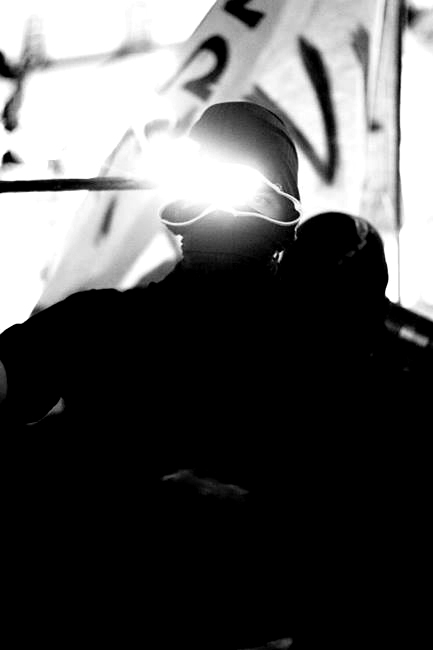
\includegraphics[width=8cm,height=10.7cm]{Imgs/img10.jpg}

\emph{Não tem arrego}, 2013
\end{center}

\section{Eu digo não}

\subsection{``Amanhã vai ser maior''}

O desejo não é uno nem múltiplo, mas
multiplicidades que operam por proliferação. E multiplicidades são, a um
só tempo, impredicáveis e substantivas. Quando saíram às ruas, o que se
ouviu dos que gostariam de organizar as revoltas como sua revolução
particular --- da direita à esquerda --- foi ``Eles não sabem o que
querem''; depois, ``Eles querem tudo'' (Cava e Cocco \emph{In}: Cava
2013: 67--68). E ``querer tudo'' aterroriza mais do que projetos
políticos niilistas. Jamais houve conversão de objeto: se é o desejo, e
não o interesse calculado, que move as multidões nas ruas, é de sua
essência querer tudo ou desejar o impossível. Esse é o momento a um só
tempo potente e perigoso do desejo --- as multiplicidades são o princípio
motor, mas nada garante que aquilo que constitui o ideado pelo desejo se
atualize porque ele opera por divergência e multiplicação. Não há, nem
pode haver, garantias --- mas perigos e prudências, conjurações e
criações que ninguém pode saber de antemão aonde vão dar --- porque o que
o desejo atualiza no campo político é sempre um efeito de criação. Por
isso, no intervalo de alguns dias em que o Movimento Passe Livre ganhou
as ruas e parecia catalisar desejos políticos heterogêneos, com
potencial de atingir escalas cada vez maiores, em que esquerda, direita
e partidos lutavam por espaço com diversos movimentos sociais urbanos
autônomos, mas também com \emph{skinheads e punks}, uma certa prudência
precisava vencer as tiranias que o desejo libertava no espaço público.
Tudo se passou como se o inconsciente coletivo, desejante, acumulado de
todos os seus fascismos e potenciais de transição, transbordasse de
repente.

Nesse momento, não podendo capitalizar os movimentos, as esquerdas ora
os qualificavam de fascistas, ora auxiliavam a esvaziar as ruas. As
manifestações da metade final de junho (Judensnaider 2013: 151--154 e
173--179) degeneram, ao menos parcialmente, em uma espécie de Marcha da
Família com Deus e a Pátria contra a Corrupção. Depois de ter falhado a
estratégia da soberania --- a porrada e a criminalização --- funcionava
disciplinarmente a da propaganda; a Imprensa havia conseguido
sobrepautar as demandas e emplacar \emph{slogans }bloqueadores da
política. O potencial político parece, então, cada vez mais intensamente
capturado por imperativos categóricos e sua má"-consciência: era preciso
rejeitar o Projeto de Emenda Constitucional nº 37, era preciso combater
a corrupção a qualquer custo, era preciso comportar"-se pacificamente,
manifestar"-se com ordem e sem violência, ajudar a identificar e prender
os vândalos etc. No fim de junho, as multiplicidades dos primeiros dias
pareciam inteiramente submetidas pelo despotismo dos corpos
bem"-comportados e pela tirania moral anticorrupção; a política
encontrava"-se inteiramente bloqueada pelo tira que cada um tem na
cabeça; o corpo era bloqueado pelo rosto que a imaginação anacrônica dos
poderes construíam como ``os caras"-pintadas''. Contra o grito efectista
de ``Não é só por 20 centavos'', do aumento do transporte público na
cidade de São Paulo --- aumento que acontecia em maior ou menor grau em
cada grande capital do Brasil --- o próprio Movimento Passe Livre, talvez
o responsável simbólico por aquilo que o imaginário político já não era
mais capaz de suturar no real, teve de ir a público mais de uma vez para
afirmar que os protestos tinham por único propósito ``os vinte
centavos''. Intelectuais, como Pablo Ortellado, também o fizeram por
mais de uma vez.

É preciso compreender que esses gestos afirmavam um item na agenda
política. Em tese, o Movimento Passe Livre só teria tido tanto sucesso
em colapsar o sistema político representativo como um todo na medida em
que possuía, como ainda hoje possui, um programa preciso nutrido por
antecedentes que não escondem o caráter multíplice do tesão político que
os sustenta.

Há alguns anos, as ruas das grandes capitais são atravessadas por
protestos multiplicadores. Nem o Movimento Passe Livre havia ``nascido
ontem'' (Pomar \emph{In: }Judensnaider 2013: 09; Movimento Passe Livre
2013: 13--14), nem havia sido a primeira experiência gestada
no seio da democracia real dos espaços urbanos. Não apenas o Movimento
Passe Livre tinha, naquele junho em que seu grito foi ouvido
internacionalmente, algo como dez anos, como tampouco é o único
movimento social que, com maior ou menor intensidade política, agregava
as infinitesimais multiplicidades de que o desejo é feito.

Há pelo menos um decênio, ao lado dos protestos pela redução das tarifas
do transporte público, ou pela implantação de políticas de tarifa zero,
gerou"-se, pouco a pouco, uma miríade de manifestações e protestos mais
ou menos efêmeros, mas de amplo espectro. Em comum, eles assumem a
gramática da defesa de direitos humanos --- talvez a única possível de um
ponto de vista intrassistêmico (Douzinas 2007: 32) --- que compreendem
desde as múltiplas pautas do Levante Popular da Juventude até as marchas
contra a presidência do Deputado Marco Feliciano na Comissão de Direitos
Humanos da Câmara dos Deputados; dos direitos reprodutivos das mulheres
--- na defesa de suas liberdades sexual e de gênero~---, bandeira das
diversas reedições das Marchas das Vadias, até manifestações pela
legalização da maconha e pelo fim da guerra contra as drogas, que ficou
conhecida como Marcha da Maconha em capitais como Rio de Janeiro e São
Paulo, entre outras.

As vitórias que o Movimento Passe Livre constrói ao longo do mês de
junho --- vitórias e visibilidades que se desdobraram em pautas muito
heterogêneas em outras cidades sob diferentes circunstâncias, como a
greve dos professores do ensino público no Rio de Janeiro --- não foram
fecundadas apenas pelo histórico do próprio movimento, mas em sua
correlação com os pequenos e incisivos buracos que cada um dos
movimentos e marchas dos últimos anos ajudaram a fazer no seio de uma
opinião pública cujas margens críticas são intensamente controladas. As
ruas, em 2013, foram um efeito de acúmulo; a luta contra o aumento, que
o Movimento Passe Livre fez reemergir como uma potência específica de
reinstauração do debate público acerca do modo de vida urbano em
praticamente todas as capitais brasileiras, foi a fenda que fez
convergir e, depois, refluir, os desejos multitudinários em diversos
sentidos potenciais.

Se as ruas foram um efeito de acúmulo, mas também de criação, o que as
miríades de protestos --- mais ou menos eficazes --- revelam é que não
apenas a gramática da defesa de direitos possui um limite interno no
instituído, mas que esse mesmo limite torna urgente distinguir o tedioso
conceito de revolução da revolta profunda de todos os corpos. Nada mais
de confundir revolução com revolta, conceitos e práxis que jamais
coincidem. Embora já esteja nas ruas desde 1999, nos protestos
antiglobalização que tiveram lugar em Seattle, o manifesto
político do século \versal{XXI} ainda está por ser escrito, e ele terá a forma de
uma fenomenologia da revolta. Uma fenomenologia da revolta como
ontologia da liberdade.

Lançar os corpos nas ruas e gritar ``3,20 é roubo!'', ou ``Ilegal
deveria ser essa sua cabeça conservadora'', constitui o gesto prático e
político em profundidade que desloca a cisão legalidades/ilegalidades
que funda as formas jurídicas consolidadas. Toda revolta é, em primeiro
lugar, a recusa profunda, afetiva e vital da repartição do lícito e do
ilícito. Por isso, ela margeia estrategicamente o ilícito, vaga nos
limiares indecisos da lei e tenta criar linhas de fuga de suas capturas
excepcionais.

O Estado e a polícia não cessam de aconselhar que os manifestantes
renunciem à violência como condição do diálogo. O Estado, porém, jamais
renuncia a ela --- a não ser estrategicamente, quando as tentativas de
criminalização falham em sua eficácia simbólica~---, embora já se tenha
atestado, por mais de uma vez, que a violência policial e estatal gera a
reação dos manifestantes (Judensnaider et al. 2013: 65--69; Cava 2013:
144). É impossível não lembrar que um refrão cantado nas ruas dizia:
``Que coincidência! Não tem polícia, não tem violência''. Esquece"-se com
frequência, mesmo entre aqueles que defendem com intransigência o
instituído, que se o Estado detém o monopólio da violência, seu titular
ainda é a massa indecisa, inconsciente e confusa que o Estado tenta
territorializar no conceito de Povo e sacralizar nos cultos ao Estado de
Direito e em seus legalismos aparentes.

A revolta profunda de todos os corpos é, em primeiro lugar, a recusa em
sujeitar"-se às formas jurídicas que ``recobrem o grande mapa das
ilegalidades''. A gramática da defesa dos direitos também tem seu
limite, e os direitos derivam da forma pura e vazia da lei que se trata
de questionar. Se a verdade profunda dos corpos é a de serem
profundamente anarquistas --- e de não cessarem de sê"-lo sob todas as
camadas de ideologia~---, o que uma tal revolta produz é uma inequação
que joga um caso contra a lei (Sutter 2018); a singularidade concreta
contra a arrogância do universal abstrato. Rebelião do caso contra as
ilegalidades que a forma da lei naturalizou como convenção e hábito
disciplinar. Qualquer movimento político se bate precisamente contra
esse limiar em que a lei formaliza e cobre o imenso mapa das
ilegalidades. Se não se bate, é porque renunciou à política --- potência
constituinte dos corpos contra o poder constituído da lei e do Estado.

\subsection{Querendo policiar}

Após as sucessivas tentativas de
criminalização do Movimento Passe Livre --- em que tudo se resume a
vandalismo sem sentido~---, a noite de 17 de junho assinala uma ``difusão
da pauta'', largamente encampada pelos meios de comunicação de massa
(Judensnaider et al. 2013: 153--155). A pauta da luta contra o aumento
nas capitais é catapultada rapidamente na direção de temas éticos que
bloqueiam, pelo menos parcialmente, o momento político: da luta contra a
corrupção à grita contra a aprovação do Projeto de Emenda à Constituição
que subtraía os poderes investigativos do Ministério Público.
Progressivamente, toda a abertura política fecha"-se em pauta ética, que
começa a se codificar e aplicar, pouco a pouco, também aos
comportamentos dos manifestantes.

Tanto que uma convocação para protestos contra o aumento das passagens
em Curitiba, em 17 de junho, no \emph{Facebook}, chegou ao ponto de
determinar uma espécie de código de conduta a ser adotado. A convocação,
além do horário, trajeto e objetivo específico da passeata regulava,
entre outros aspectos, o caráter pacífico da manifestação e conclamava
os manifestantes a registrarem atos de depredação patrimonial a fim de
que a polícia pudesse identificar os responsáveis. Tornado explícito e
incorporado ao cerne do movimento, o código de ética provocava um
curto"-circuito entre polícia e protesto. O tira na cabeça dos
curitibanos havia vencido o revolucionário. Na mesma noite do dia 17,
porém, grupos de manifestantes se dispersam do trajeto e investem contra
estações"-tubo no caminho do centro histórico da cidade em direção ao
Centro Cívico, picham as paredes externas do Palácio do Governo estadual
e quebram algumas vidraças, sob o protesto de alguns manifestantes que
tentam impedi"-los e, mais tarde, limpariam as pichações voluntariamente.
Curitiba e seu Centro Cívico eram a dupla prova de que certo código de
ética havia sido adotado contra os vandalismos; ao mesmo tempo em que os
vandalismos emergiam e persistiam, o aparente triunfo do tira na cabeça
de certos manifestantes era o sintoma de que uma nova repartição interna
de forças surgia. A política era absorvida pela ética e pelos seus
códigos.

No início de setembro, na cidade do Rio de Janeiro, os professores da
rede municipal de ensino público entram em greve como signo de sua
recusa contra a aprovação iminente de um plano de carreiras e salários
pela administração de Eduardo Paes. Em um momento em que as cinzas de
junho ainda rescendiam, a greve se torna mais que mera paralisação e
negação à prestação de um serviço público; à recusa ao trabalho
agrega"-se uma estratégia coletiva de ocupação da praça que se localiza
em frente à sede da Câmara Municipal da cidade do Rio de Janeiro. As
ruas levavam para fora das salas de aula os encontros proliferantes
entre professores e seus alunos (Cava 2013: 131) que, como resposta do
Estado, não obtinham nada além da tirania dos procedimentos legislativos
e a pacificação forçada do aparelho repressivo do Estado.

Os sucessivos episódios de violência policial contra as ocupações e
manifestações levam as multidões das praias e das cidades, das favelas e
prédios de apartamentos, dos batalhadores e jovens universitários a se
reencontrarem nas ruas em defesa das bandeiras do magistério estadual,
contra o consenso eleitoral com que o pacto Dilma"-Cabral"-Paes blindava a
proposta legislativa que acarretava retrocessos no âmbito dos direitos
sociais dos servidores do professorado. Se os atos de vandalismo já
estavam por toda a parte, desde junho, é apenas em setembro que eles se
apresentam ao grande público das mídias como tática de ação direta das
ruas. A multidão de professores, alunos e manifestantes se reencontrava
no deserto das ruas, segundo os afetos de um agenciamento concreto
completamente diferente daquele de junho --- mas sob um perfume sutil de
sua atmosfera intempestiva. Ali, nas ruas do Rio, a mesma multidão que
meses atrás condenava o método das ações diretas --- nem sempre utilizado
como tática black bloc; muitas vezes, protagonizado por policiais e
infiltrados (os P2), que objetivavam deslegitimar politicamente os
protestos --- reconheceu, finalmente, nas margens da tática, que \emph{o
black bloc era uma ética}.

Sem qualquer bula de valores, prescrições ou códigos morais, os
professores do Rio eram apresentados ao black bloc como a uma ética do
acontecimento. Quando a repressão policial tinha início com a explosão
de bombas de efeito moral, gás lacrimogêneo e uso ostensivo de armas de
baixa letalidade, como \emph{spray }de pimenta, armas municiadas com
projéteis de borracha e os clássicos cassetetes dos batalhões de Choque,
o black bloc formava a linha de frente das manifestações, ou depredava
alguma coisa chamando a atenção da polícia, a fim de que os
manifestantes menos preparados para os confrontos diretos pudessem fugir
para as ruas contíguas. Não por acaso, entre os próprios professores ---
que se autointitulavam em uma ironia simbólica ``Tropa de Profes'',
contra a Tropa de Choque --- surgia o ``Black Prof''. Não exatamente um
destacamento de professores black blocs --- embora isso tenha sido
possível (Cava 2013: 127--128)~---, mas uma maneira de reconhecer e
agradecer o apoio tático que o black bloc fornecia aos professores em
sua luta por direitos; também, um devir interno ao próprio movimento. O
black bloc do Rio e de Niterói reencontrava os princípios radicais de
sua genealogia autonomista, da década de 80 (Judensnaider et al. 2013:
37--38), e que pautaram novas modalidades de ação durante a luta
antiglobalização em Seattle: ser o bloco tático de autodefesa da
multidão contra as ações policiais \emph{anti"-riot}.

Se junho havia sido marcado paradoxalmente como reabertura política
potencial do espaço público, mas também como recrudescimento a um código
de disciplina e conduta mais ou menos adotado em cada uma das cidades
rebeldes, as contracondutas black blocs de setembro, reinventando"-se
como ética, canibalizaram o \emph{ethos} médio. Enquanto as mídias
insistiam no projeto de disciplinarização das condutas e
espetacularização dos movimentos --- afinal, havia funcionado de alguma
maneira no recente episódio da luta contra o aumento~---, o black bloc
era o \emph{happening }que garantia a integridade física dos
manifestantes no Rio contra o Choque. A ação direta recolhia e dobrava
por dentro a ética do choque. No agenciamento concreto entre polícias e
black blocs, o choque entre os corpos se transformava em modelo ético
espinosano, gerava afetos insuspeitos.

\begin{figure}[h]
\centering
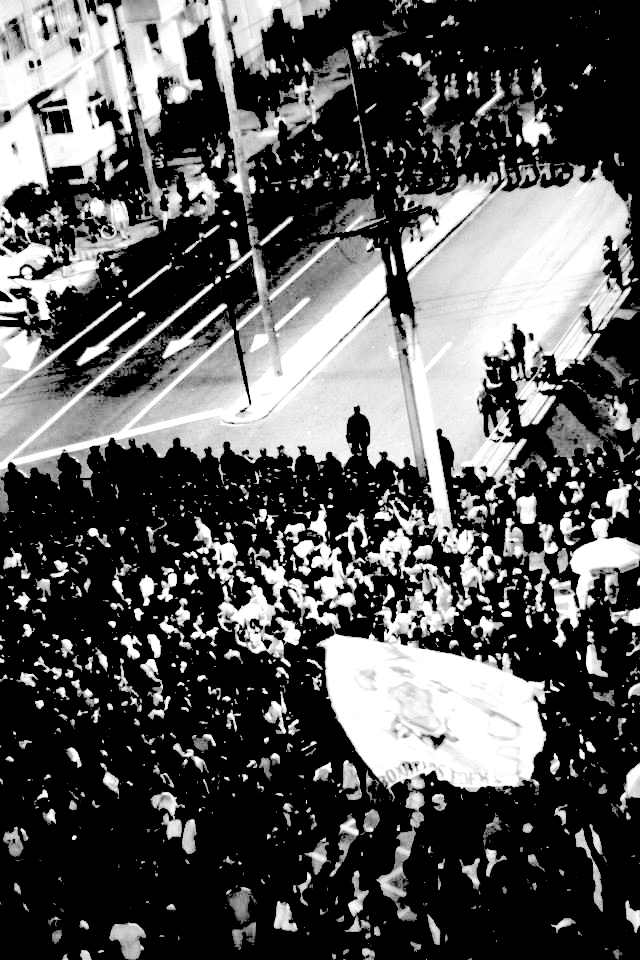
\includegraphics[width=9cm,height=10.92cm]{Imgs/img11.jpg}
\emph{Modelo}, 2013
\end{figure}

\section{Eu digo não ao não}

\subsection{Happening}

Era outubro de 1967. Caetano Veloso e os Beat Boys
subiam ao palco do \versal{III} Festival da Música Popular Brasileira, da \versal{TV}
Record de São Paulo, para apresentar \emph{Alegria, Alegria. }Desde o
primeiro \emph{riff} de guitarra, foram hostilizados com as vaias
uníssonas que vinham da plateia universitária politizada. E Caetano,
sozinho, caminhou alguns momentos contra o vento --- até que a marchinha
\emph{pop} furasse o gosto e se tornasse uma das gratas surpresas
daquele festival, ``apesar'' das guitarras. No mesmo festival em que
Caetano apresentara \emph{Alegria, Alegria,} Gilberto Gil subiu ao palco
com Os Mutantes para interpretar \emph{Domingo no Parque}. Pelo mesmo
motivo --- os instrumentos demoníacos que Os Mutantes empunhavam~---, a
plateia vaia a execução da canção do início ao fim. Aparentemente, as
guitarras elétricas vandalizavam a forma"-canção da Moderna Música
Popular Brasileira; nem \emph{Domingo no Parque}, de Gilberto Gil, nem
\emph{Alegria, Alegria}, de Caetano Veloso, eram tão conteudistas ou
engajadas como \emph{Ponteio}, de Edu Lobo, ou \emph{Roda"-Viva},
de Chico Buarque.

Três meses antes, Elis Regina e Jair Rodrigues, que apresentavam \emph{O
fino da bossa}, haviam participado de uma Marcha contra a guitarra
elétrica que o iê"-iê"-iê popularizava rapidamente entre os jovens
``não"-engajados''. Marchava"-se contra a invasão cultural imperialista,
em favor da tradição, para ``defender o que é nosso''. Mesmo que não se
dessem conta, os jovens universitários marchavam de braços dados com o
mesmo patriotismo dos coturnos militares que esmagavam suas utopias. Sem
estar convencido, Gil participara a convite de Elis Regina --- segundo
ele, ``não sabia dizer não para Elis''. Caetano achava tudo ``muito
estranho''; assistira a marcha passar da janela de um hotel, em
companhia de Nara Leão, que definiu a mobilização como ``integralista''
e ``fascista''. O mesmo povo que antes havia marchado contra a guitarra
elétrica, encontrava nos \emph{riffs }e referências \emph{pop} da marcha
alegórica \emph{cool }de Caetano, e nos arranjos cinematográficos
einsensteinianos de Gil e Duprat em \emph{Domingo no Parque}, o
ponto de partida em que o corpo"-a"-corpo com as guitarras e o choque de
gosto encaminhavam o público no sentido insuspeito de uma radical
mudança de sensibilidade (Favaretto 2007: 20--24).

Um ano mais tarde, trocas: enquanto Gilberto Gil apresentava
\emph{Questão de ordem }acompanhado pelos Beat Boys, Caetano\emph{
}Veloso apresentava \emph{É proibido proibir} no \versal{III} Festival
Internacional da Canção com Os Mutantes, e sua canção protagonizava um
novo choque de gosto. Caetano tem os cabelos compridos e imensos colares
de contas sobre o colo; vestido com roupas de plástico coloridas, seu
corpo sobe ao palco fazendo uma dança erótica, emulando uma relação
sexual. Acompanhado dessa vez pelas guitarras de Os Mutantes, a plateia
virou as costas para o palco em reprovação moral enquanto alguns
atiravam tomates, ovos, pedaços de madeira contra o grupo. Os Mutantes
revidaram tocando de costas para a plateia. E Caetano, emputecido, em
meio ao arranjo de \emph{É proibido proibir}, grita o \emph{mote }de sua
canção, e acusa a plateia --- em sua maioria, formada por estudantes
universitários politizados: ``Vocês estão querendo policiar a Música
Popular Brasileira! Se vocês, em política, forem como são em estética,
estamos feitos!'', dizia Caetano. Corpo do novo contra o gosto
incrustado nos corpos: ``Vocês aplaudem hoje uma música que não
aplaudiriam um ano atrás''. Os carros estavam incendiados.
\emph{Happening }ético contra os códigos de ética. ``Vocês não estão
entendendo nada!''.

\subsection{Ethica}

Assim como a Tropicália reinseria o corpo na música e
reinventava a canção por meio de um procedimento irônico --- que não era
senão uma maneira muito particular de dobrar e desdobrar a cafonice da
era do rádio~---, a potência específica da ética black bloc encontra"-se
em recusar, não sem efeitos irônicos, todo código de conduta em proveito
de uma ética radicalmente corporal.

Nem humanos, nem animais, mas informes, os corpos black blocs formam com
as ruas um agenciamento concreto que faz passar a política como um devir
que atravessa tanto corpos quanto espaços urbanos. Os corpos se
multiplicam e se encontram nas ruas. As ruas definem o \emph{ethos }dos
fluxos, ou lugar em que se vive, logo convertido no ponto de junção em
que a afirmação do direito à cidade (Harvey 2013: 28) coincide com as
singularidades de seu potencial constituinte.

A cidade compõe um \emph{ethos }duplamente estratégico: campo
físico do encontro\footnote{``A cidade é usada como
  arma para sua própria retomada: sabendo que o bloqueio de um mero
  cruzamento compromete toda a circulação, a população lança contra si
  mesma o sistema caótico de transporte das metrópoles {[}\ldots{}{]}''
  (Movimento Passe Livre São Paulo \emph{In: }Maricato et al. 2013:
  16).} e lugar da produção e reprodução das forças que o
definem\footnote{``As cidades são o principal local
  onde se dá a reprodução da força de trabalho'' (Maricato 2013: 19).
  Embora a força de trabalho seja uma das forças de um corpo, não parece
  suficiente para defini"-lo. Sob esse aspecto, cf. a diferença que
  Deleuze e Guattari (2007: 72--84) estabelecem entre arma e ferramenta.
  Aproveitando a definição de Ermínia Maricato, talvez fosse o caso de
  afirmar que ``As cidades são o principal local em que se processam as
  produções das forças e sua conversão em afetos; isto é, armas''.}.
\emph{Ethos} que promove o encontro e o contágio entre corpos
anarquistas, e entre estes e os corpos policiais --- o que não deixa de
definir, em sentido espinosano, o agenciamento concreto que uma ética
supõe. Se a ética é corporal, uma física dos corpos, de suas forças e de
seus arranjos de forças, ela assume a forma de uma \emph{ética do
choque}. Um choque se produz a cada encontro microfísico entre múltiplos
corpos e as multiplicidades que se compõem com seus afetos e desejos. O
mesmo modelo físico de uma ética de corpos capaz de descrever o choque
entre Tropicália e forma"-canção, entre gosto inscrito nos corpos e nova
formação de sensibilidade, ou entre seus instrumentos técnicos (guitarra
elétrica e violão), descreve os encontros entre corpos vândalo e
policial, manifestante e choque, repressão e ação direta, ou entre
violência juridicamente estruturada e tática horizontal de autodefesa
das multidões contra o Um. Em uma ética, tudo o que importa se passa no
\emph{entre} --- \emph{entre} corpos vândalos e rostos policialescos;
\emph{entre }o choque da ética e uma ética corporal do choque;
\emph{entre} o desejo de múltiplo e as capturas do Um. Sai de cena o
modelo ético dos valores em proveito de um modelo físico de encontros
dos corpos, aumentos e diminuições de potências, sujeição das paixões
que afetam um corpo ou multiplicação e sedição de suas forças. Contra a
ética das bulas de princípios e códigos de condutas, as contracondutas
black blocs fundam o vandalismo como um dos instrumentos afirmativos a
serviço de uma recusa radical: contra o capital, contra o Estado que o
suporta, contra a propriedade --- em uma palavra: contra a sociedade
dividida, a sociedade policiada, contra o Um (Clastres 2011). Se, fora
das disciplinas, e para além de qualquer cisão antropológica, o corpo é
um bicho, a dissolução do rosto, a rasura das identidades, a defesa
contra o controle, o anarquismo dos corpos e as ações diretas contra o
Um e seus representantes formam mais que uma ética; formam uma etologia
black bloc que coincide com suas contracondutas campais.

Classicamente, a etologia é definida como o estudo do comportamento
animal. Em certo sentido, superficial e culturalmente muito determinado,
ela ainda faria reverberar uma cisão antrópica. Porém, abandonemos as
concepções culturais em proveito da coincidência sem resíduos entre
política e ontologia que definia toda política como uma
\emph{beaglepolitik}. Se todo corpo é um bicho --- de laboratório
(operação do poder) --- ou simplesmente bicho (teoria dos corpos
anarquistas), devemos atentar mais à pregnância etimológica de
``etologia'' que a seu significado culturalmente decantado. No sentido
em que o propomos, uma etologia black bloc se definira em pelo menos
três sentidos:

\begin{enumerate}
\item A contraconduta que exprime uma vida contra a forma que ela adquire
no \emph{ethos}. A conduta que rasura os códigos morais é a expressão de
uma potência corporal profunda que age contra os modos de vida
naturalizados, e que elege por campo de emergência precisamente no lugar
em que se vive (um dos sentidos etimológicos de \emph{ethos}), a cidade,
em que toda cisão entre o público (\emph{pólis}) e o privado
(\emph{oikos}), como entre vida política (\emph{bios}) e vida orgânica
(\emph{zoé}), perdem o sentido em proveito do corpo e suas potências ---
móbeis ontológico"-políticos dessas expressões;

\item Um corpo que contesta sua forma contém mais do que a mera oposição
entre um corpo humano ou animal poderia exprimir. ``Humano'' ou
``animal'' são predicados culturais ocidentais que definem campos
específicos de forças: o homem é definido em função da potência de
sentir, imaginar, calcular, trabalhar, falar, morrer etc.; tudo está
dado e fechado. Trata"-se, antes, de um corpo"-bicho --- sede de
multiplicação das forças --- contra a antropogênese. Nesse sentido,
inteiramente novo, toda ética --- relação e inter"-relação dos corpos --- é
uma etologia;

\item Em um mundo humano, ser integralmente seu corpo --- um bicho --- é mais
que uma contestação, uma contraconduta. Esse corpo genealógico e ao
mesmo tempo novo, feito de pele e pelos eletrizados, carne e músculos
livres, se forja no encontro intensivo com a impotência de forças sempre
já constituídas. Nos termos de sua etologia, um black bloc define"-se de
acordo com uma ética profundamente espinosana na medida em que um bloco
de corpos encontra sem cessar outros blocos de corpos --- humanos,
policiais, morais, revoltosos, não"-violentos ou irascíveis. Esses
encontros produzem efeitos de criação que tanto podem ser destrutivos
quanto criativos. Puro tesão político, de um encontro pode nascer tanto
repressão e sujeição quanto um beijo \mbox{impossível}.
\end{enumerate}

\subsection{Teoria da ação direta}

Em 1970, Hannah Arendt publicava um
texto destinado a analisar a questão da violência no âmbito da política.
\emph{On violence} propunha uma distinção conceitual radical entre
violência (\emph{Gewalt}) e poder (\emph{Macht}), e apontava um arsenal
crítico contra o elogio sartreano, feito à época das barricadas
estudantis, à ``violência incontrolável do homem recriando"-se a si
mesmo'' (Arendt, 2011, p.~27--28). Arendt reconhecia a força disruptiva
da violência como instrumento político, mas não sem se acautelar contra
os efeitos destrutivos da ``fúria louca'' que, em Fanon, transformava em
homens os ``desgraçados da terra'', ou sem demonstrar que isso
pressupunha considerar a história como um processo contínuo de
automatismos das ações humanas que apenas um evento violento poderia
interromper (Idem, p. 47 e p. 22).

No mesmo ensaio, Arendt definia a violência como ``o agir sem
argumentar, sem o discurso ou sem contar com as consequências'', mas,
estranhamente, parecia encontrá"-la mais ao lado dos jovens estudantes
franceses de 68, ou do movimento \emph{Black Power}, do que do lado do
Estado repressor ou das instituições sociais racistas. Na raiz de sua
repulsa está o fato de que, diferentemente dos advogados de uma
criatividade vital que a violência encerraria, a ação violenta seria
essencialmente destrutiva, incapaz de criar novas condições de ação,
pensamento e discurso em comum. A violência pode mudar o mundo, liquidar
o velho, mas é destituída da capacidade de fazer nascer o novo.
Encontraríamos o novo mais do lado da faculdade de agir em conjunto e do
poder, do que do lado da essência negativa da violência.

De 2013 para cá, a sensibilidade social continua a ser seletivamente
arendtiana: ``A primeira coisa que {[}o black bloc{]} causa em
mim é um sentimento de violência. Eles estão mudos e são fortes. É
exatamente como Arendt caracteriza a violência: ela ocorre na ausência
da palavra, ela é muda'', afirmava Yara Frateschi (2013, p.~182--183),
que, apesar dessa declaração, tampouco queria, em pleno 2013,
``antecipar o que são os Black Blocks''. Essa ``sensibilidade
arendtiana'' parece ter percorrido o campo social e definido uma chave
policial de interpretação dos levantes de 2013/2014 marcada por uma
identificação simples entre a tática black bloc e uma concepção
laxista de violência. Sua estranha característica: jamais se perguntar
sobre os Eichmanns dos batalhões de choque, sobre o mutismo com
que os chefes dos poderes executivos da União e dos Estados autorizavam
as ações policiais violentas, ou sobre as responsabilidades coletivas
acerca da crescente burocratização da vida; isto é, ``a forma de governo
na qual todas as pessoas estão privadas da liberdade política, do poder
de agir'' (Arendt, 2011, p. 101).

Alguns anos antes, em \emph{Eichmann em Jerusalém}, Arendt gerava a
\emph{banalidade do mal} como conceito"-chave que permitia explicar a
pane moral que os fascismos europeus deflagraram ao transformar o horror
em hábito; caçar judeus era uma operação policial de rotina (Sutter,
2017, p. 90) e Adolf Eichmann, finalmente, não era nada além de um
policial comum. Ele jamais foi o monstro moral e inumano que se esperava
encontrar sentado no banco dos réus, mas uma figura tão burocrática
quanto ordinária do \emph{law enforcement} do Estado alemão.

Se formos fiéis a Arendt, e não à ``sensibilidade arendtiana'' que ainda
circula, reconheceremos que os levantes de 2013/2014 constituíram
eventos, ``ocorrências que interrompem processos e procedimentos de
rotina'' (Arendt, 2011, p. 22) em que os homens reuniram"-se com seus
pares, agiram em concerto, aventuraram"-se em algo novo. Isso porque o
poder encontrava"-se do lado dos governados; os governantes, por sua vez,
não cessaram de responder à reunificação do corpo social ao poder
específico que o define com violência institucionalizada. Por isso, é
preciso desassociar os termos black bloc e violência. Como a
integral do corpo social, a tática está mais próxima de uma operação de
retomada do poder dos governados, do que da ação violenta. O black
bloc, como segmento tático das lutas de Junho e além, jamais foi a
violência manifesta e incorporada, ou o duplo simétrico da violência
policial do Estado, como mesmo as análises mais benévolas gostariam de
fazer acreditar. Não foi nem um desastrado fenômeno espetacular
débordiano, nem a emergência aterradora de aparências transitórias na
luz ordinariamente tão exclusiva do espaço público. Ao contrário, o
black bloc foi, e continua a ser ainda hoje, a prova atlética,
eticamente autolimitada, e povoada de perigos, das condições mais
profundas da política: não ``aparecer'', como quisera Arendt (2011, p.
87), mas \emph{presentar} em toda a sua radicalidade \emph{um ato
simples em que ação e discurso se curto"-circuitam.} Eis o significado
profundamente político de qualquer ação direta: apresentar ação e
discurso no \emph{corpus} de um ato simples, em que a ação mesma
constitui um ato de tomada do direito à palavra recusada pelas
democracias representativas, e em que a palavra se encontra inteiramente
expressa na ação disruptiva que a reivindica.

O fato de que certa conformação da sensibilidade social possa
considerá"-lo um resto mudo da antipolítica, ou uma manifestação violenta
e niilista, se deve aos efeitos policiais da burocracia que governa as
sensibilidades coletivas. As rotinas e a ordem policial dos lugares
constituem"-se separando a ordem das palavras e a ordem das ações;
reservando a alguns --- os representantes e os especialistas --- o lugar
exclusivo do discurso, às custas do silenciamento compulsório dos
muitos, e a outros, o papel executivo e efetivamente violento de atuar
os implementos que transfiguram os discursos em palavras de ordem. Por
isso, o black bloc é parte essencial do evento que consiste na
ação concertada do corpo social de retomar o poder à violência ordinária
das burocracias que, hoje, já não podem mais ser definidas como ``o
domínio de Ninguém'', uma ``tirania sem tirano'' (Arendt, 2011, p. 103),
mas como o consórcio espúrio entre as instituições do Estado e o
ecumenismo de mercado que sequestram, segundo uma ordem policial que o
define, as capacidades de pensar, dizer e agir em comum. As ações
diretas rompem o tecido sensível das repartições entre as potências de
ver, dizer e fazer que definem uma dada formação social, e podem apelar
a um começo.

Às sensibilidades conformadas por uma ordem policial, o exercício dessa
capacidade coletiva por tanto tempo forcluída --- e que não cessa de
retornar --- só pode ter a aparência de um niilismo violento praticado
contra todos os axiomas, inclusive os que delimitam a divisão entre o
\emph{político }e o\emph{ antipolítico,} estabelecida em função de uma
sensibilidade policial. Eis o sintoma de que estamos no coração dos
``afetos da ordem'' e manipulamos em comum as condições para constituir
outras partilhas do sensível (``outra ordem dos afetos'').

É isto, o político: estarmos às voltas com a capacidade comum para o
evento, para interromper uma dada ordem sensível e os procedimentos de
rotina pelos quais ela se conserva. O político é a emergência do
\emph{démos} no seio da burocracia e da ordem policial: é a abertura
para novas condições do viver junto que começam pelo desafio essencial
ao qual toda ação direta tenazmente se dedica: dar um fim à polícia para
que a política volte a entrar, mesmo que precariamente, ainda uma vez na
constelação dos possíveis.

\subsection{Lixo lógico}

Depois de estudar o samba, o pagode, a bossa nova
e o funk, nos últimos meses de 2012, Tom Zé lançava ``Tropicália, Lixo
Lógico''. Um disco que, da repetição dos procedimentos, mais que dos
gestos fundacionais do tropicalismo --- como uma espécie de tropicofagia
imanente, mas não autofágica~---, oferecia"-lhe uma espécie de amplo novo
corpo no qual sua pequena e irredutível diferença poderia proliferar. A
paródia de \emph{Enquanto seu lobo não vem}, de Caetano, é exemplar.
Tudo se passa como em um conto de fadas. Nele, a pureza da Música
Popular Brasileira do final dos anos sessenta passeia na floresta
``Enquanto seu lobo não vem''. Porém, seu lobo --- a Tropicália --- logo
entra na festa. Como um corpo"-bicho, tentador e de ``pelos fortes'', mas
que, de fato, ``não comeu ninguém'', a festa promove o encontro entre
uma tropicália lupínica e a pureza da forma"-canção (lupicínica?). A
pureza e o lobo da pureza se tornam, em um outro segmento da canção de
Tom Zé, as encarnações risíveis do embate superficial entre duas
estruturas de pensar: uma, ocidental, conhecida desde os primeiros dias
de escola, equacional e aristotélica; outra, moçárabe, própria dos
analfatóteles, inequacional e diferencial. Tudo se passa como se o
apreendido (aristotélico ou ocidental) e o desejo natural, curioso e
insistente (analfatotélico ou moçárabe), fossem forçados a uma
correspondência que não se podia recusar. Ao resolver ``também com
nossas armas a questão'', ao propor ``uma moçárabe possível solução'', o
resultado quase igual gerava sempre uma pequena diferença, um extra"-ser,
algo como um lixo lógico que, jogado por tão longo tempo --- a duração de
toda uma infância, que corresponde tanto à ausência de \emph{logos}
quanto ao silêncio que marca o inconsciente --- ``no poço do hipotálo'',
só podia acumular"-se a ponto de invadir ``o córtex do arteiro''.

Ao contrário do que supôs toda a teoria marxista do conflito social, uma
revolução não se faz apenas com ideias claras e distintas, nem com
teleologias da história. Não recusamos suas equações, mas é preciso
resolver também com nossas armas a questão. Uma revolução se produz
sempre como efeito de acúmulo e efeito de criação; o lixo lógico é sua
matéria primeira e a revolta profunda de todos os corpos, sua condição.

Em 1932, quando Bergson (2001: 1213) se depara com a afirmação de Émile
Faguet, segundo a qual a Revolução Francesa foi feita, não em nome da
liberdade e da igualdade, mas ``porque se morria de fome'', a pergunta que
jamais cessou de ecoar desde então foi: ``E por que, a partir de um
certo momento, não mais desejamos morrer de fome?''. Como quase tudo, em
Bergson, a resposta se encontrava nos termos do enunciado: ``não mais
\emph{desejamos }morrer de fome''. Algo se passou da ordem de um devir
das formas de vida --- de maneira semelhante como algo se altera no gosto
estético. Na medida em que as intenções com que uma ideia é lançada
continuam a imantá"-la por um longo tempo, é preciso lembrar que, mesmo
para Bergson, toda fórmula democrática origina"-se da revolta, exprime um
desejo revolucionário, formula o que deve ser a fim de liquidar o que é
--- e, nesse sentido, implica um trabalho prático a um só tempo negativo
e positivo. Como não enxergá"-lo na expressividade --- estética, mas
também ética e política --- das ações diretas, tática black bloc contra
formas de viver e modos de sensibilidade que, de repente, se tornaram
intoleráveis?

Ao compreender a Tropicália, ao mesmo tempo, como efeito de criação e
efeito de acúmulo (lixo lógico), a intuição estética de Tom Zé
permitiria reunir Bergson e Lapoujade sob uma simples epígrafe: o corpo
revolucionário é um corpo que não aguenta mais, porque ``não aguentar
mais'' é uma forma de tocar a própria definição de corpo (Lapoujade 2002: 83), assim como o que ainda não sentimos é a matéria de toda sensação.
Em um corpo, a potência se encontra liberada do ato: anti"-Aristóteles,
moçárabe concepção da potência, diferença diminuta que é mais uma gota
``na história milionária de todos os erros''. Uma revolução começa por
uma potência emancipada do ato em um corpo que não aguenta mais o que se
impõe do exterior (organização), como as dobras de sua própria alma
(subjetivação), e a revolta profunda de todos os corpos converte seu
cansaço secular no limiar positivo da recusa: ``é desde sempre e para
sempre que não aguentamos mais, se é desde sempre e para sempre que
resistimos, então esta resistência é um profundo fortalecimento, a
constante de um limite ou de um `último nível'.'' (Lapoujade 2002: 85).

Um corpo é, já, uma ética: erupção contínua do encontro com outros
corpos: luz, oxigênio, comida, sons e palavras. Tudo o corta. Tudo faz
borda. E, no entanto, é esse corpo que não aguenta mais que não cessa de
responder a Bergson: ``primeiro, é preciso suportar o insuportável'',
efeito de acúmulo, ou memória dolorífera (``eu digo sim'') liminar no
seio da qual todo o ser passa a agir, em que a recusa (``eu digo não'')
se converte em positividade (``eu digo não ao não'') explosiva: \emph{é
proibido proibir}. Ponto em que o desejo de multiplicar o múltiplo de
uma etologia black bloc se torna a apologia de sua \emph{ethica}.

\chapter{Devir black bloc}

\begin{center}
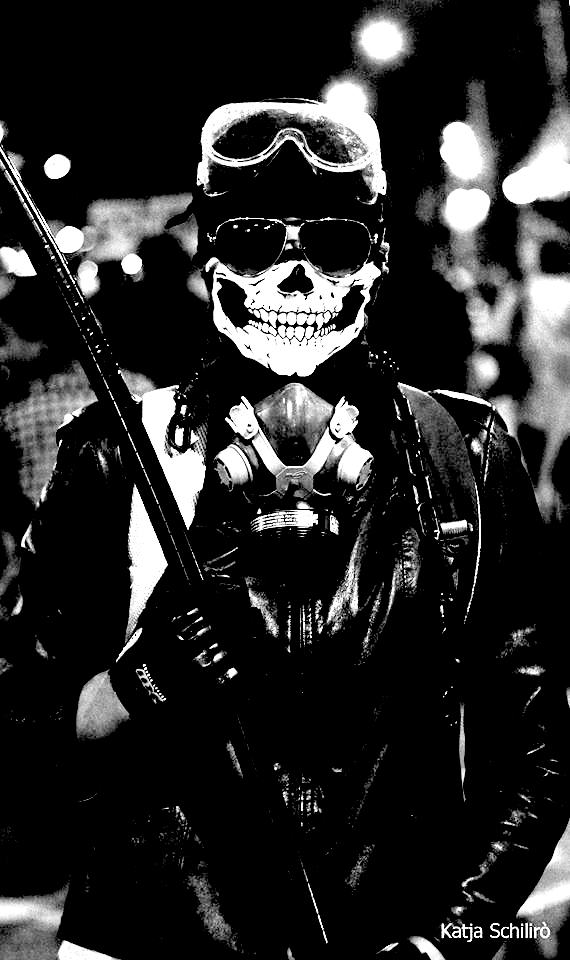
\includegraphics[width=7cm,height=11.7cm]{Imgs/img12.jpg}
\end{center}

Como acontecimento, Junho de 2013 teve duas metades, mas boa parte dos
analistas dedicou"-se mais a uma delas do que à outra. Pensar Junho como
acontecimento é pensá"-lo de acordo com forças que se produzem por
divergência ou bifurcação: de um lado, há os determinismos sociais, as
séries causais, os fatores atuais que conduzem a Junho e à sua atmosfera
de indignação; de outro, há a abertura de campos de possíveis outrora
insondáveis, há o mergulho social na sua instabilidade constituinte
(Deleuze 2003: 215--216) e a transformação de um corpo social estável em
um campo social aberto a transições. Um acontecimento conjuga, portanto,
duas metades: as formas em que se atualiza e as forças que alteram as
formas sem se esgotarem nelas.

Junho foi um acontecimento encarnado, um grito coletivo e múltiplo que
denunciava o intolerável cotidiano, mas foi também o fenômeno de
vidência coletiva e a alteração da partilha do sensível que até então
soldava o desejo coletivo à sua sujeição. Eis a dimensão afetiva e
social que as análises tradicionais mal alcançam, pois captam um
fenômeno mais como ato que como potência; porque se prendem às cadeias
de causalidade histórico"-sociais, quando ``o próprio acontecimento está
em {[}\ldots{}{]} ruptura com as causalidades {[}\ldots{}{]}'' (Deleuze 2003: 215). O que se dissimula sob o truísmo confortável dos intérpretes que
se debatem entre definir Junho como um evento inédito ou ligado a uma
cadeia de causas sociais e políticas é o fato de que não cessamos de
fechar os olhos para o acontecimento puro, para as lógicas em
profundidade que movem as insurgências sociais e para o elemento de
ruptura de que elas são portadoras. As categorias maiores, e as formas
régias do pensamento, não cessam de impor que façamos vistas grossas.

Não é raro que Junho apareça definido a partir de traços negativos.
Junho teria sido, então, o ciclo de protestos do sem: sem partidos, sem
líderes, sem representação, sem previsão de uma institucionalidade
futura, sem unidade, sem causas aparentes; em uma palavra, um bizarro
fenômeno social, ou cultural, mas não político, porque vocalizava
demandas que buscavam extorquir resultados da esfera política formal,
sem dialogar com ela na sua linguagem particular. Outras vezes --- e aqui
se vai mais longe~---, Junho aparece como um acontecimento que resulta de
uma cadeia de causalidades político"-sociais razoavelmente definidas: a
ascensão social de uma classe média baixa subproletária e precarizada,
mas incluída pela via de uma cidadania consumidora, a revolta de
segmentos médios contra os escândalos de corrupção nacionais, demandas
auto"-organizadas pela diminuição da tarifa dos transportes públicos que
aparecem como estopins de demandas mais profundas, como o direito à
cidade, e.\,g. Traços negativos e causalidades conceituais que produzem,
por vias divergentes, o mesmo resultado: presos às expressões
atualizadas de Junho, deixam escapar a metade virtual do acontecimento;
analisando"-o como ato, deixam de analisá"-lo como potência.

Essas análises não devem ser descartadas. No registro atual do fenômeno,
as análises negativas são até certo ponto úteis para questionar o que
deixamos de ser, embora percam de vista os traços positivos. As análises
causais permitem entrever um corpo social aparentemente homogêneo e
estável no ponto em que é atravessado por fissuras que estariam na
origem de transformações macropolíticas. Embora úteis, ambos os modelos
de análise terminam por perder de vista o essencial: questionar em que
consiste o aspecto transformador e revolucionário dessas rupturas que
atravessam um corpo social até então estável? Que devires fissuram uma
formação social a ponto de romper o seu equilíbrio precário? Mas,
principalmente, o que esses devires exigem de nós? Que outros modos de
vida, de relações em comum, que outros povos e mundos por vir esses
devires enunciam em sua maquinação coletiva? Em Junho de 2013, fugimos
--- socialmente, politicamente~---, mas para onde? Eis a pergunta que mais
nos fizemos, e que menos pudemos responder, esmagados pela surpresa,
pelo erro, pela incompreensão ou pela má consciência analítica.

Todos os erros e insuficiências que se produziram em relação a Junho
também se produziram em relação ao black bloc, o que o converte em um
analisador geral de Junho em potência. No entanto, é preciso entender em
que termos. Assim como os acontecimento podem ser analisados sob o ponto
de vista do ato ou da potência, o mesmo se passa com os ``grupos
sociais''. No entanto, analisar os grupos sociais em virtude de sua
identidade de grupo, de suas ações e práticas, de sua cultura social e
política, seria ainda permanecer refém dos limites etnográficos. Assim
como é preciso compreender Junho mais como potência do que como ato,
mais como devir do que como resultado de uma cadeia de causalidades, é
preciso compreender o black bloc mais como algo que se instala em uma
linha de fuga de um campo social do que como grupo.

Talvez esse exercício sirva para completar as análises etnográficas com
sua desejosa porção política e metafísica --- uma vez que o black bloc,
na nossa tradição recente, é o que não merece ser matéria do pensamento,
entregue à opinião e ao juízo. Trata"-se menos de analisar um grupo
social --- tarefa da etnografia --- do que de analisar os sentidos que o
``social'' recebe em um grupo; isto é, cartografar as linhas de fuga
impessoais, definidoras de um campo social, que o black bloc faz passar.
Eis o que quer dizer fazer do black bloc um analisador de Junho:
compreendê"-lo como uma singularidade em conexão com as forças do campo
social; estimar seus potenciais para desterritorializar e
reterritorializar o social, perguntando sobre o seu modo relacional:
``qual o recado de Junho de que o black bloc poderia ser a expressão?''

Já não se trata de fazer falar as pessoas ou as classes por detrás das
máscaras. Trata"-se desenvolver a máscara como um ponto de vista interno
ao campo social, e fazer falar este ponto de vista como máquina de
enunciação coletiva; descrever seus traços positivos; estimar as novas
relações sociais e políticas que ele performa ou pré"-forma; tentar estar
à altura da matéria social em movimento que o black bloc exprime. Tentar
definir ``que política se produz a partir da recusa, do não, do
negativo?''. ``Que fugas o black bloc prepara para o social e o
político?''. Gostaria de desenvolver três hipóteses para essas questões
a partir da descrição de três devires comuns ao campo social, a Junho de
2013 e ao black bloc: os devires -ninguém, -qualquer um e -todo mundo.

\section{Devir"-ninguém}

Quem somos nós nas metrópoles do capitalismo
cognitivo, nas usinas sociais do trabalho precário e nas sociedades de
controle? \emph{Quem} é uma questão anacrônica. Quando nossa vida passa
a ser administrada em escala planetária como multiplicidades abertas
quaisquer (Deleuze 2014: 366), deixamos de ser o que fomos para as
formações soberanas e disciplinares --- sujeitos ou corpos físicos~---, e
nos tornarmos dados, massas, amostras, informações, bancos, imagens
(Deleuze 2008: 222). Isto é, tornamo"-nos \emph{ninguém}, pois os
dispositivos que hoje nos asseguram alguma identidade, o fazem de
maneira difusa e fragmentária (Agamben 2014: 85), segundo os limites
imanentes que o capital opera por expansão e deslocamento no campo
social (Deleuze e Guattari 2007: 127). Os processos de subjetivação e
os modos da identidade passam a se constituir de forma integrada ao
capitalismo global, tornando os processos de subjetivação e de relação
social um campo singular de lutas políticas. Indivíduos infinitamente
divisíveis, dividuais, focos emissores de signos, de comunicação e
constelações de afetos conectados em redes planetárias e geradores de
valor. O interior das vidas integra hoje o terreno das operações do
capital e do antagonismo político.

Nesse panorama desolador em que um sistema de dominação passa ao
interior de nós mesmos e se apresenta sob a sedutora forma do
``empreenda"-te a ti mesmo'' (Dardot e Laval 2016: 396), não faltou quem
tenha declarado --- em paralelo com o esmorecimento do ciclo de revoltas
globais --- a morte de toda possibilidade de revolução e de resistência
interna ao capitalismo (Han 2014). É curioso que hegelianos e
heideggerianos costumem encarregar"-se de bom grado dos obituários
políticos do nosso século; sinal de que, por mais que sejam bons
diagnosticadores, têm muito pouco a dizer sobre o devir"-revolucionário
das pessoas.

Entretanto, algumas linhas de ruptura foram expostas no interior dos
processos de subjetivação capitalísticos. Decretar a impossibilidade das
revoluções em um sistema de poder que se estabiliza pela suave sedução
das promessas de prosperidade pessoal em contraste com a dura
normalização das disciplinas deveria fazer"-nos ler em sentido
politicamente forte a prescrição de Deleuze (2008: 220): ``Não se deve
perguntar qual é o regime mais duro, ou o mais tolerável, pois é em cada
um deles que se enfrentam as liberações e as sujeições''. Não há como
estimar as sujeições e as fugas senão na imanência de uma formação
social e de seu sistema de dominações. Se as revoluções já não parecem
possíveis, talvez isso se deva menos à representação abstrata da morte
do seu futuro do que ao fato de que os novos movimentos sociais produzem
uma outra lógica política: a lógica dos levantes e das revoltas, que têm
mesmo muito pouco a ver com as clássicas organizações revolucionárias.

Os levantes e as revoltas não obedecem à dialética das revoluções, mas à
lógica horizontal e transversal das insurgências. No nível da
subjetivação, sua ação política consiste em realizar o que às revoluções
parece ser impossível: converter aspectos das subjetividades controladas
em processos insurgentes de subjetivação política (Hardt e Negri 2014:
49). Isso só pode ocorrer no seio do corpo social no qual nos
encontramos inscritos, como uma experimentação social e política capaz
de responder a demandas mais universais, ligadas ao domínio planetário
do capital.

Talvez o traço que mais distinga o black bloc sejam suas
características visuais: as máscaras e as roupas pretas. Características
que dizem respeito à tática de intervenção nas ruas, que remetem ao
simbolismo das bandeiras negras, e possuem razões muito pragmáticas ---
como poder realizar uma ação direta e fugir para o interior do bloco
negro, permanecendo invisível (Dupuis"-Deri 2014). Aí está em jogo um uso
político do \emph{devir"-ninguém }que atravessa as sociedades de
controle: contra os poderes e as subjetividades constituídas, é possível
devir um ninguém que eles não querem que sejamos e apontá"-lo
precisamente contra os ninguéns em que eles nos transformaram.

Dissimular o rosto com máscaras ou tecidos, homogeneizar os corpos em
vestes negras, reconverte o anonimato da vida nas grandes metrópoles e
dos circuitos capitalistas do entretenimento e do espetáculo, que
reservam a notoriedade como prêmio pela útil sujeição de alguns poucos.
Não é à toa que o black bloc reivindica um ``anonimato
notório'', de maneira coletiva e agindo no coração das metrópoles
e das instituições do capital financeiro.

O que torna as sociedades de controle eficazmente difusas e modulares é
a sua capacidade de exercer controle em praticamente qualquer espaço e
em qualquer nível, macro ou micrológico. Seus dispositivos sociotécnicos
vigiam desde as massas anônimas e anárquicas até as rugas de um rosto na
multidão. Isso faz do rosto mais do que um signo de fixação da
identidade pessoal --- ele se converte em uma máscara biopolítica. É
nesse sentido que o ponto de vista da máscara black bloc sobre o
rosto constitui uma forma de vandalismo primeiro.

Desfazer"-se do rosto, sobrepor"-lhe uma máscara para desbloquear a ação
direta, é converter a cifra anônima dos controles em fator de
insurgência ingovernável. É recusar ativamente os signos da identidade
fragmentária das rostificações em benefício de uma política em que os
ninguéns podem formar multidões informes e confusas. A verdade profunda
das multidões baseia"-se na recusa ativa do rosto em proveito das
singularidades irredutíveis de um corpo social criativo, múltiplo,
nômade, anônimo, potente, inclassificável e incoercível. O rosto é uma
política e desfazê"-lo é nosso destino, porque no seio de uma cultura
identitária, a política se define como uma guerra de guerrilhas entre
corpos indisciplinados e rostos despóticos.

Trata"-se de uma política contra o rosto, mas apenas na medida em que ela
o faz entrar em relação com outras forças biopolíticas insondáveis.
Devir"-ninguém, do rosto ao corpo, é a condição para um devir
radicalmente democrático nas sociedades de controle, e seu ponto de
partida e de conversão são as subjetividades controladas. É
significativo que dissimular o rosto tenha se convertido em uma condição
prática para fazer política nas democracias pós"-espetaculares; é ainda
mais significativo que as máscaras torçam o anonimato cotidiano das
vidas contra os seus controles segundo as vias divergentes de um
devir"-ninguém absolutamente outro.

\section{Devir"-qualquer um}

No entanto, devir"-ninguém é uma condição ainda
negativa. Consiste em apagar o rosto como dispositivo por meio do qual
as disciplinas e os controles biopolíticos governam e administram a vida
em comum e o seu valor. O corpo tampouco salva. O rosto é o elemento
formal a que o corpo aliena a sua potência, e a máquina de rostificar é
estatal. Há corpos inteiramente rostificados (Deleuze e Guattari 2008: 35);
isto é, impotentes. Se o rosto é uma política e as máscaras são
um ponto de vista contra o rosto que libera a ação e torna os corpos
ingovernáveis, é preciso, de um lado, definir o estatuto dessas
subjetividades emergentes e, de outro, reencontrar os corpos sob os
rostos desfeitos. Eis o ponto em que ultrapassamos a negatividade: a
antipolítica da rostidade, efetuada por um devir"-ninguém, cede lugar a
uma práxis dos corpos anarquistas: um devir"-qualquer um.

Sob as máscaras e as identidades dissolvidas, um adepto da tática dizia
``agora somos bloco. {[}\ldots{}{]} deixo de ser eu e me junto
a eles'' (Solano et al. 2014: 87). O que isto quer dizer? Que as
identidades fragmentárias e dispersivas produzidas pelo capitalismo
ecumênico, liberadas do controle e de seus sistemas de pertença de
maneira acontecimental e efêmera, já não podem ser dados, massas,
índices, pontos abstratos em uma curva de normalidade biopolítica, ou
elementos dividuais passíveis de controle. Tornam"-se singularidades
flutuantes, abertas a individuações e agenciamentos coletivos livres;
convertem"-se em corpos insubmissos outra vez capazes da ação política
porque relativamente insujeitos aos controles. Eles se definem mais pela
variação contínua de uma potência de agir e de dissimular"-se no bloco, e
pela potência de variar a ação taticamente em função de necessidades
estratégias das situações (Dupuis"-Déri 2014: 63) que por identificações
individuais ou coletivas.

Então, o que para os controles eram fragmentos dispersos de identidades,
agora funciona como uma composição variável de corpos definidos pelo seu
poder de afetar e de serem afetados. O agenciamento de corpos
relativamente livres dos controles, reunidos à sua potência específica,
produz um bloco; um bloco é uma composição em variação contínua no qual
se produz um devir"-qualquer um. Eis o que significa ``deixar de ser
eu'', ``juntar"-se a eles'' (essa terceira pessoa do plural que permanece
impessoal) ou ``ser bloco''. É constituir uma singularidade que compõe
com outras singularidades segundo a sua capacidade de afetar e ser
afetada, de acordo com seus graus de potência (liberdade) ou de
impotência (servidão) (Espinosa 2009).

A composição das potências e impotências entre esses corpos insubmissos
pode fazer"-nos tocar noções de democracia de pensadores tão distantes
quanto Platão. O ideal platônico de governo sempre foi assombrado pelo
advento da democracia que, no livro \versal{VIII} da República, aparece como a
antítese de qualquer forma de governo político e como a reversão de
todas a relações bem ordenadas que estruturam as sociedades humanas
(Rancière 2014: 50--51).

``Por meio da revolta, e sem qualquer motivo aparente'', as democracias
fazem desaparecer as divisões que permitiam hierarquizar governantes e
governados, homens e mulheres, pais e filhos, cidadãos e estrangeiros,
professores e alunos, velhos e jovens, animais e homens (Platão 2011:
1729--1730 {[}562d--563d{]}). A democracia é a forma de governo múltipla e
anárquica em que o desejo, o prazer e os afetos das multidões governam,
liberados da domesticação da ``boa ordem viril'' que a educação pela
música e pela ginástica teria imposto às almas e à pólis (livros \versal{III} e
X). Quando os pobres vencem os oligarcas e partilham igualmente o
governo e as magistraturas, geralmente por sorteio, a plebe governa por
decretos assembleares. Trata"-se de um Estado em que não há necessidade
alguma de mandar e de obedecer, em que se reparte uma igualdade radical.

Nas ruas, quando se passa das singularidades anônimas à sua composição
em bloco, do devir"-ninguém ao devir"-qualquer um, corpos quaisquer são
reunidos à potência outrora alienada à forma do Estado. Essa é uma
operação que produz, a um só tempo, a restauração da multiplicidade dos
corpos no comum e a restauração do comum na multiplicidade dos corpos. Eis
aí o efeito profundamente político de devir"-qualquer um: a democracia,
compreendida como governo múltiplo das singularidades quaisquer, que
repudiava os governos eleitos em proveito dos sorteados, permanece
aberta ao governo de qualquer um, independentemente da posse de títulos
ou propriedades.

O que os analistas chamaram de ``falência da representação política''
como principal sintoma de Junho recupera, então, todo o seu sentido
positivo. A marca de Junho não está na recusa da representação --- esta é
tão somente o sinal de uma recusa mais profunda e democrática: está,
antes, na recusa da alienação do poder do corpo social à forma do Estado
(Clastres 2003: 219--220). Nas sociedades ditas primitivas, toda a
política dos selvagens resume"-se à luta para que o Estado não advenha, e
para que esta alienação não se opere (Clastres 2011: 138). Em nossos
Estados oligárquicos de direito (Rancière 2014: 92), caracterizados
pelo sequestro do poder político em uma esfera separada do corpo
social,\footnote{``La théorie de la souveraneité du peuple
  contient en elle"-même sa négation. Si le peuple tout entier était
  vraiment souverain, il n'y aurait plus de gouvernement, plus des
  gouvernés. Le souverain serait réduit à zéro. L'État n'aurait plus la
  moindre raison d'être, il s'identifierait avec la société''
  (Guérin 2016: 27),} a política não deixa de ser, para nós, algo do
que fora para as sociedades primitivas: recusar o sequestro do poder
social em uma esfera separada chamada Estado; contraefetuar todo o
dimorfismo social e político; afirmar uma igualdade radical sem
precedentes e transformar essa afirmação em enunciado coletivo e em
gesto político que pode ter \emph{qualquer um} por porta"-voz.

\section{Devir"-todo mundo}

A verdadeira horizontalidade de Junho de
2013 não está na dinâmica formal das manifestações de rua; este é o
horizontalismo fraco com o qual os intelectuais de Estado querem que nos
confortemos. Assim como há em Junho, e nos black blocs, uma
recusa do Estado como forma de consolidar a separação entre um corpo
social e seu poder, há também um horizontalismo forte, a instauração de
dinâmicas assembleares e da ocupação de espaços públicos que,
politicamente, criam balões de ensaio para uma democracia radical por
vir. Eis o terror de Platão e dos rostos despóticos: que os corpos
anarquistas emerjam e vençam; que eles se auto"-organizem e se
autogovernem; e pior, que possam tomar todo mundo em um devir.

E se nossos corpos se portassem como pontos de expressão das relações de
poder que efetivamente os atravessam? Se recuperassem, mesmo que de
maneira efêmera, a potência ingovernável que deles foi separada para
constituir os governos? Criaríamos outras composições para as forças,
relações e corpos? Suscitaríamos outros encontros, uma nova ética,
outros mundos, nascidos do gérmen apodrecido das nossas sociedades
divididas e policiadas? Eis os problemas políticos radicais que as ações
diretas propõem.

Devires constituem as linhas de fuga que definem um campo social. Desse
ponto de vista, devires são forças que abrem uma formação social para
além da sua matéria formada. Elas mobilizam a potência contra o ato, o
virtual contra o atual, a política contra o ser, a realidade contra as
ficções estruturais e o campo social contra os contratos. Isso permite
compreender o black bloc não como um subconjunto de Junho, mas
como um terreno de experimentação política, um campo de variação
contínua que mantém uma relação de composição com as linhas de fuga que
definem um campo social. Por isso, o black bloc não é responsável
pelos devires de Junho, mas pode constituir um analisador geral na
medida em que se instala em suas principais linhas de fuga.

A linha de fuga que Junho de 2013 fez passar --- sobre a qual as
caravanas black blocs se instalaram --- consistiu no limite
imanente de todas as fugas políticas: um \emph{devir"-todo mundo.} Nem
fascismo, nem niilismo, nem denuncismo, nem espetáculo: as ações
diretas, voltadas à destruição de propriedades e símbolos do capitalismo
financeiro, e também contra o Estado, não eram imagens, mas exercícios
profanatórios de poderes que encontramos dispersos e em funcionamento
por toda a extensão do grande consórcio legal entre mercado e Estado. Os
poderes de erguer barreiras, de impedir acessos, de constranger
liberdades, de fazer fluir as ruas ou consumir e destruir mercadorias e
propriedades. Em um regime de conexão assimétrica com as formas de
exercício do poder sequestrado do campo social pela forma"-Estado, as
ações diretas instauraram cintilações divergentes, arrancaram partículas
diferenciais.

Quando os black blocs afirmavam que ``violento é o Estado'', ``o
mercado'', ``o transporte público'' ou ``o dia a dia'', ``não as ações
diretas'', propõem uma distinção entre poder e violência (Corrêa 2017:
45); afirmam que a única condição para que se possa exercer o poder sem
violência é que ele não seja sequestrado na forma do Estado e na ficção
da representação; isto é, que ele permaneça inseparável das
multiplicidades que compõem um dado campo social. As ações diretas são
tão simbólicas quanto afirmativas e reais. Elas não são um duplo
simétrico da violência do Estado; são manifestações de poder e práticas
de sua aberta divergência em relação à violência sistêmica. ``Destruir
um símbolo'' é afirmar a coincidência entre ação e discurso; praticar a
distância real entre o exercício do poder e o da violência. O
black bloc não faz ``como'' o Estado; compõe uma nova paisagem
sensível nas metrópoles com as polícias, os controles, o capital e a
propriedade.

Mais do que \emph{devir"-ninguém}, o que está em jogo no black bloc
é arrancar às formas de subjetividade imanentes aos controles de nossa
época um \emph{devir"-imperceptível}. É nesse ponto que o anonimato do
black bloc ganha todo o seu sentido e potência políticos.
Dessubjetivar"-se, \emph{devir"-ninguém} sempre nos expõe ao perigo de
sermos rapidamente enquadrados pelos controles (Cocco e Tascheto 2017:
43). No entanto, \emph{devir"-ninguém} pode ser a máscara --- jamais imune
a riscos e perigos --- sob a qual se dissimula um aspecto essencial do
\emph{devir"-todo mundo}: a capacidade de fazer um movimento real passar
despercebido (Deleuze e Guattari 2007: 74--75).

Deleuze (1998: 10) não cessou de dizer que devir não é imitar. Devir é
``extrair partículas, entre as quais instauramos relações de movimento e
repouso, de velocidade e lentidão, as mais\emph{ próximas }daquilo que
estamos em vias de nos tornarmos, e através das quais nos tornamos''
(Deleuze e Guattari 2007: 64). Isso exige que se crie uma zona de
vizinhança --- ou de indeterminação --- entre aquilo que se é, o lugar em
que se está, a vida que se vive e o que tudo isso vem a ser. Portanto,
as grandes transformações são as que se deslocam anônimas, que parecem
fazer parte de uma paisagem prosaica porque instauram uma zona de
vizinhança entre o que se é e o que se vem a ser. Um devir não comporta
a sabedoria do camaleão, que se colore com a paisagem, mas a malícia
elusiva dos cefalópodes, que tingem o oceano para fugir. Não imitar a
paisagem, mas compor com ela; pintá"-la com as cores da fuga que vem. Os
20 centavos e, mais tarde, Amarildo, nomearam deslocamentos anônimos do
desejo social que se tornou capaz de perceber os aspectos intoleráveis
da vida em comum. Junho pintou uma paisagem e nos introduziu na
atmosfera de indignação que o aumento ou o desaparecimento de Amarildo
requeriam.

\emph{Devir"-todo mundo} implica, então, duas coisas: de um lado, passar
despercebido pelas formas \emph{a priori} da sensibilidade atual; de
outro, instaurar uma composição capaz de fissurar essa sensibilidade de
modo imperceptível. As sensibilidades policiadas só conseguem perceber
um fenômeno como o black bloc nos seus próprios e exclusivos
termos. Por isso, toda a má literatura sobre criminosos mascarados e
sobre a sua suposta solidariedade com os circuitos capitalísticos do
espetáculo. Toda essa paranoia intelectual é incapaz de explicar tanto
os devires quanto as expressões concretas de um campo social. Isso
talvez se deva menos à incapacidade teórica dos intérpretes e mais à
potência do black bloc para \emph{devir"-imperceptível:} sua
capacidade política está em fazer passar despercebido o movimento real
de Junho precisamente ao permanecer sob as luzes dos holofotes.

Sensibilidades policiais não apenas não percebem o que se passa, como
não percebem que algo se passa. Para percebê"-lo, é preciso ter captado
os movimentos políticos ou reais do campo social com o qual essas
subjetividades insurgentes compõem. É preciso compreender como elas
criam uma nova paisagem com a qual fazem contato; como produzem mundos
comunicantes, mas que permanecem imperceptíveis sob o velho casaco do
constituído.

O \emph{devir"-todo mundo} tem, pois, dois sentidos que se compõem entre
os planos do transcendental e do empírico: um
\emph{devir"-imperceptível}, que consiste em pintar o mundo com a sua
cor, preparar uma paisagem; mas também, o ato de \emph{instalar todo
mundo em uma fuga, }produzir uma constelação de alternativas ao mesmo
tempo distinta e interior àquela paisagem. Eis o que explica que se
tenha compreendido tão mal o black bloc, especialmente os que o
veem como procelárias dos tempos do espetáculo. O black bloc
compõe com um campo social permeado por uma sensibilidade policial e
espetacular. Por isso, sob o seu regime, tudo o que se pode perceber,
ver e dizer sobre o black bloc dá"-se nos termos dos seus próprios
referenciais: niilismo político, espetáculo e crime.

Quando uma subjetividade política se choca com a sociedade em que a
política foi sequestrada por uma oligarquia de Estado, toda ação
política será chamada ``antipolítica''. Quando uma ação direta se choca
contra uma sociedade policiada, todo extravasamento de seus códigos terá
por nome ``crime''. Quando um fenômeno social se choca contra uma
sociedade espetacular e pós"-industrial, todo\emph{ possível }será visto
como imagem reiterativa. Portanto, não deve soar paradoxal que o
black bloc permaneça em uma anônima notoriedade. Em uma sociedade
de ninguéns que lutam para ser alguém, sua singularidade permanece
clandestina na medida em que qualquer um pode compor com um black
bloc e em que o black bloc poderia compor com qualquer um;
isto é, com todo mundo.

Nas margens dos legalismos ilegais do capitalismo, garantidos pelo
consórcio com o Estado e suas polícias, composições de singularidades
perseveram na potência de prefigurar uma outra vida em comum: sem a
propriedade, sem o grande capital, sem a polícia, sem as sujeições
hierárquicas e os dimorfismos que as sustentam, sem o Estado, que
sequestra o poder do corpo social em uma esfera separada, e que separa
os corpos anárquicos daquilo que eles podem. Talvez um pouco como dizem
os pichadores que se recusam a entrar nas galerias de arte (``Fui crime,
serei poesia''), também o black bloc possa dizer depois de Junho:
``querem"-nos crime porque muito antes teremos sido, e seremos,
política''.

%\chapter{Procuram-se armas}
\begin{bibliohedra}
\hedramarkboth{procuram-se armas}{}

\tit{AGAMBEN}, Giorgio. \emph{Mezzi senza fine: Note sulla politica}.
Torino: Bollati Boringhieri, 1996.

\tit{\_\_\_\_\_}. \emph{L'aperto: L'uomo e l'animale}. Torino: Bollati
Boringhieri, 2002.

\tit{\_\_\_\_\_}. \emph{Homo sacer: O poder soberano e a vida nua \versal{I}}.
Tradução de Henrique Burigo. Belo Horizonte: Editora da \versal{UFMG}, 2007.

\tit{\_\_\_\_\_}. \emph{O que resta de Auschwitz} (Homo Sacer \versal{III}).
Tradução de Selvino J. Assman. São Paulo: Boitempo, 2008.

\tit{\_\_\_\_\_}. \emph{Nudez}. Tradução de Davi Pessoa. Belo
Horizonte: Autêntica, 2014.

\tit{ARANTES}, Paulo. \emph{O novo tempo do mundo}. São Paulo: Boitempo, 2014.

\tit{ARENDT}, Hannah. \emph{Origens do totalitarismo}. Tradução de
Roberto Raposo. São Paulo: Companhia das Letras, 2009.

\tit{\_\_\_\_\_}. \emph{Sobre a violência}. Tradução de André
Duarte de Macedo. 3ª ed. Rio de Janeiro: Civilização Brasileira, 2011.

\tit{ARISTÓTELES}. \emph{Les politiques}. Tradução e apresentação de Pierre Pellegrin. 2ª ed. Paris: \versal{GF} Flammarion, 1993.

\tit{AVELAR}, Idelber. ``The June 2013 uprisings and the waning of
Lulismo in Brazil: Of antagonism, contradiction, and oxymoron''.
\emph{Luso"-Brazilian Review} 54: 1, 2017.

\tit{BERGSON}, Henri. \emph{Œuvres: Édition du centenaire}. Paris:
Presses Universitaires de France, 2001.

\tit{\_\_\_\_\_}. \emph{Duração e simultaneidade}. Tradução de Cláudia
Berliner. São Paulo: Martins Fontes, 2006.

\tit{BUCCI}, Eugênio. \emph{A forma bruta dos protestos: Das
manifestações de junho de 2013 à queda de Dilma Rousseff em 2016}. São
Paulo: Companhia das Letras, 2016.

\tit{CAVA}, Bruno. \emph{A multidão foi ao deserto: as manifestações
no Brasil em 2013 (jun--out)}. São Paulo: Annablume, 2013.

\tit{CAVA}, Bruno; \versal{MENDES}, Alexandre. \emph{A constituição do comum:
Antagonismo, produção de subjetividade e crise no capitalismo}. Rio de
Janeiro: Revan, 2017.

\tit{CHAUÍ}, Marilena. ```Black blocs' agem com inspiração fascista, diz
filósofa a \versal{PM}s do Rio''. \emph{Folha de S.\,Paulo}, 27/08/2013.

\tit{CLASTRES}, Pierre. \emph{A sociedade contra o Estado: Pesquisas
de antropologia política}. Tradução de Theo Santiago. São Paulo: Cosac
Naify, 2003.

\tit{\_\_\_\_\_}. \emph{Arqueologia da violência: Ensaios de
antropologia política}. Tradução de Paulo Neves. São Paulo: Cosac Naify, 2011.

\tit{COCCO}, Giuseppe. \emph{Mundobraz: O devir"-mundo do Brasil e o
devir"-Brasil do mundo}. Rio de Janeiro: Record, 2009.

\tit{\_\_\_\_\_}. \emph{KorpoBraz: Por uma política dos corpos}. Rio de
Janeiro: Mauad X, 2014.

\tit{COCCO}, Giuseppe; \versal{TASCHETO}, Marcio. ``Eu (não) sou ninguém: A
subjetividade sem nome''. \emph{Kalagatos}. Fortaleza, v. 14, nº 2, 2017. p.
37--57.

\tit{CORRÊA}, Murilo Duarte Costa. ``Para dar um fim à polícia''.
\emph{Lugar Comum}. Rio de Janeiro, nº 50, junho/setembro, 2017. p. 33--48.

\tit{\_\_\_\_\_}. ``Rafael Braga Vieira: O singular e os universais da
polícia''. \emph{Dilemas: revista de estudos e de conflito social}. Rio de
Janeiro, v.\,11, nº\,2, 2018.

\tit{DARDOT}, Pierre; \versal{LAVAL}, Christian. \emph{A nova razão do mundo:
Ensaio sobre a sociedade neoliberal}. Tradução de Mariana Echalar. São
Paulo: Boitempo, 2016.

\tit{DELEUZE}, Gilles. \emph{Spinoza et le problème de l'expression}.
Paris: Presses Universitaires de France, 1968.

\tit{\_\_\_\_\_}. \emph{Foucault}. Paris: Presses Universitaires de
France, 1983.

\tit{\_\_\_\_\_}. \emph{Nietzsche e a filosofia}. Porto: Rés"-Editora, 2001.

\tit{\_\_\_\_\_}. \emph{Deux régimes de fous: Textes et entretiens
(1975--1995).} Paris: Les Éditions de Minuit, 2003.

\tit{\_\_\_\_\_}. \emph{Diferença e repetição}. Tradução de Luiz
Orlandi e Roberto Machado. 2ª ed. Rio de Janeiro: Graal, 2006.

\tit{\_\_\_\_\_}. \emph{Conversações (1972--1990)}. Tradução de Peter Pál
Pelbart. São Paulo: Editora 34, 2008.

\tit{\_\_\_\_\_}. \emph{El poder: Curso sobre Foucault}. Tomo \versal{II}. Buenos
Aires: Cactus, 2014.

\tit{DELEUZE}, Gilles; \versal{GUATTARI}, Félix. \emph{Mil platôs: Capitalismo e
esquizofrenia}. Vol. 4. Tradução de Suely Rolnik. São Paulo: Editora 34, 2007.

\tit{\_\_\_\_\_}. \emph{Mil platôs: Capitalismo e
esquizofrenia}. Vol. 5. Tradução de Peter Pál Pelbart e Janice Caiafa.
São Paulo: Editora 34, 2007.

\tit{\_\_\_\_\_}. \emph{O que é a filosofia? }Tradução de
Bento Prado Júnior e Alberto Alonso Muñoz. São Paulo: Editora 34, 2007.

\tit{\_\_\_\_\_}. \emph{Mil platôs: Capitalismo e
esquizofrenia}. Vol. 3. Tradução de Aurélio Guerra Neto, Ana Lúcia de
Oliveira, Lúcia Cláudia Leão e Suley Rolnik. São Paulo: Editora 34, 2008.

\tit{DELEUZE}, Gilles; \versal{PARNET}, Claire. \emph{Diálogos.} Tradução de Eloisa
Araújo Ribeiro. São Paulo: Escuta, 1998.

\tit{DERRIDA}, Jacques. \emph{Mal de arquivo: Uma impressão freudiana}.
Tradução de Cláudia de Moraes Rego. Rio de Janeiro: Relume"-Dumará, 2001.

\tit{DESCOLA}, Phillipe. \emph{Par de là nature et culture. }Paris:
Gallimard, 2005.

\tit{DOUZINAS}, Costas. \emph{Human rights and empire: The political
philosophy of cosmopolitanism}. New York: Routledg"-Cavendish, 2007.

\tit{\_\_\_\_\_}. \emph{Philosophy and resistance in the crises:
Greece and the future of Europe}. Cambridge: Polity Press, 2013.

\tit{DUPUIS"-DÉRI}, Francis. \emph{Black blocs. }Tradução de Guilherme
Miranda. São Paulo: Veneta, 2014.

\tit{ESPINOSA}, Baruch de. \emph{Tratado teológico"-político}. Tradução
de Diogo Pires Aurélio. São Paulo: Martins Fontes, 2008.

\tit{\_\_\_\_\_}. \emph{Tratado político}. Tradução de Diogo Pires
Aurélio. São Paulo: Martins Fontes, 2009.

\tit{FAVARETTO}, Celso. \emph{Tropicália, alegoria, alegria}. 4ª ed.
Cotia: Ateliê Editorial, 2007.

\tit{FIGUEIREDO}, Ney. ``Os empresários e os movimentos de rua''. \emph{In:} 
\versal{FIGUEIREDO}, Rubens (Org). \emph{Junho de 2013: A sociedade enfrenta o
Estado}. São Paulo: Summus Editorial, 2014. p. 61--72.

\tit{FRATESCHI}, Yara; \versal{RIBEIRO}, Nádia Junqueira. ``Entrevista: Yara
Frateschi''. \emph{Inquietude}. Goiânia, vol. 4, nº 2, jul/dez, 2013.
p. 178--187.

\tit{FOUCAULT}, Michel. ``Qu'est"-ce que la critique? Critique et
Aufklärung''. \emph{Bulletin de la Société française de philosophie}.
Tradução de Gabriela Lafetá Borges. Vol.
82, nº 2, abr/jun 1990 (Conferência proferida em 27 de
maio de 1978). p. 35--63.

\tit{\_\_\_\_\_}. \emph{Dits et écrits}. Paris: Quarto/Gallimard, 2001.

\tit{\_\_\_\_\_}. ``Le philosophe masqué''. \emph{In}: \emph{Dits et
écrits. }\versal{II} (1976--1988). Paris, Quarto/Gallimard, 2001. p. 923--929.

\tit{\_\_\_\_\_}. \emph{Em defesa da sociedade.} Tradução de Maria
Ermantina Galvão. São Paulo: Martins Fontes, 2002.

\tit{\_\_\_\_\_}. \emph{Hermenêutica do sujeito}. Tradução de Márcio
Alves da Fonseca e Salma Tannus Michail. São Paulo: Martins Fontes, 2006.

\tit{\_\_\_\_\_}. \emph{Segurança, território, população}. Tradução de
Eduardo Brandão. São Paulo: Martins Fontes, 2008.

\tit{\_\_\_\_\_}. \emph{História da sexualidade: a vontade de saber 1}.
Tradução de Maria Thereza da Costa Albuquerque e J. A. Guilhon
Albuquerque. 19ª ed. Rio de Janeiro: Graal, 2009.

\tit{\_\_\_\_\_}. \emph{Vigiar e punir: Nascimento da prisão}. Tradução
de Raquel Ramalhete. 40ª ed. Petrópolis: Vozes, 2012.

\tit{GUÉRIN}, Daniel. \emph{L'anarchisme: De la doctrine à la
pratique}. Paris: Éditions Gallimard, 2016.

\tit{GOHN}, Maria da Glória. \emph{Manifestações de junho de 2013 no
Brasil e praças dos indignados no mundo}. Petrópolis: Vozes, 2014.

\tit{HAN}, Byung"-Chul. ``Por que hoje a revolução não é possível?''
\emph{El País}, 03/10/2014.

\tit{HARDT}, Michael; \versal{NEGRI}, Antonio. \emph{Declaração: Isto não é um
manifesto}. Tradução de Carlos Szlak. São Paulo: n-1 edições, 2014.

\tit{HOBBES}, Thomas. \emph{Do cidadão}. Tradução de Renato Janine
Ribeiro. São Paulo: Martins Fontes, 2002.

\tit{\_\_\_\_\_}. \emph{Os elementos da lei natural e política}.
Tradução de Bruno Simões. São Paulo: Martins Fontes, 2010.

\tit{JUDENSNAIDER}, Elena et al. \emph{Vinte centavos: A luta contra
o aumento}. São Paulo: Veneta, 2013.

\tit{LA BOÉTIE}, Etienne. \emph{Discurso da servidão voluntária.
}Tradução de Laymert Garcia dos Santos. São Paulo: Brasiliense, 1982.

\tit{LACAN}, Jacques. ``D'une question préliminaire à tout traitement
possible de la psychose''. \emph{In:} \emph{Écrits.} Paris: Éditions du
Seuil, 1966. p. 531--583.

\tit{LAPOUJADE}, David. ``O corpo que não aguenta mais''. \emph{In: }\versal{LINS},
Daniel; \versal{GADELHA}, Sylvio (Orgs.).\emph{ Nietzsche e Deleuze: Que pode o
corpo}. Rio de Janeiro: Relume"-Dumará, 2002. p. 81--90.

\tit{LAZZARATO}, Maurizio. \emph{As revoluções do capitalismo}.
Tradução de Leonora Corsini. Civilização Brasileira, 2006.

\tit{MARICATO}, Ermínia et al. \emph{Cidades rebeldes: Passe livre e
as manifestações que tomaram as ruas do Brasil}. São Paulo: Boitempo e
Carta Maior, 2013.

\tit{MELMAN}, Charles. \emph{O homem sem gravidade: Gozar a qualquer
preço}. Entrevistas por Jean"-Pierre Lebrun. Tradução de Sandra Regina
Felgueiras. Rio de Janeiro: Companhia de Freud, 2003.

\tit{NEGRI}, Antonio. \emph{De volta: Abecedário biopolítico}.
Entrevistas com Ande Dufourmantelle. Rio de Janeiro: Record, 2006.

\tit{\_\_\_\_\_}. \emph{La fábrica de porcelana: Una nueva
gramatica de la política}. Traducción de Susana Lauro. Barcelona: Paidós, 2008.

\tit{NEGRI}, Antonio; \versal{COCCO}, Giuseppe. \emph{Glob(AL): Biopoder e luta
em uma América Latina globalizada}. Tradução de Eliana Aguiar. Rio de
Janeiro: Record, 2005.

\tit{NEGRI}, Antonio; \versal{HARDT}, Michael. \emph{Império}.
Tradução de Berilo Vargas. 8ª ed. Rio de Janeiro: Record, 2006.

\tit{NIETZSCHE}, Friedrich Wilhelm. \emph{Genealogia da moral: Uma
polêmica}. Tradução de Paulo César de Souza. São Paulo: Companhia das
Letras, 2008.

\tit{NOGUEIRA}, Marco Aurélio. \emph{As ruas e a democracia: Ensaios
sobre o Brasil contemporâneo}. Rio de Janeiro: Contraponto, 2013.

\tit{NUNES}, Rodrigo. ``June n'est pas fini''. \emph{In: Les temps modernes},
nº 678, 2014. p. 4--23.

\tit{OLIVEIRA}, Ana de (Org.). \emph{Tropicália ou panis et
ciercencis}. São Paulo: Iyá Omin, 2010.

\tit{ORTELLADO}, Pablo. ``A negação de Junho, 4 anos depois''. \emph{Folha
de S.\,Paulo}, 18/06/2017.

\tit{PINTO NETO}, Moysés. ``A hipótese anarquista''. \emph{In: Sopro}, nº
96. Setembro de 2013.

\tit{POMAR}, Marcelo. ``Não foi um raio em céu azul''. \emph{In:}
\versal{JUDENSNAIDER}, Elena et al. \emph{Vinte centavos: A luta
contra o aumento}. São Paulo: Veneta, 2013. p.~08--19.

\tit{PINHEIRO}, Paulo Sérgio. ``Governo democrático, violência e estado
(ou não) de direito''. In: \versal{BETHELL}, Leslie (Org.). \emph{Brasil: Fardo do
passado, promessa do futuro. Dez ensaios sobre política e sociedade
brasileira}. Rio de Janeiro: Civilização Brasileira, 2002. p.~237--269.

\tit{PLATÃO}. \emph{A república}. Tradução de Maria Helena da
Rocha Pereira. 13ª ed. Lisboa: Fundação Calouste Gulbenkian, 2012.

\tit{\_\_\_\_\_}. \emph{Œuvres complètes, sous la direction de Luc
Brisson}. Paris: Flammarion, 2011.

\tit{RANCIÈRE}, Jacques. \emph{O desentendimento: Política e
política}. Tradução de Ângela Leite Lopes. São Paulo: Editora 34, 1996.

\tit{\_\_\_\_\_}. \emph{Ódio à democracia. }Tradução de Mariana
Echalar. São Paulo: Boitempo, 2014.

\tit{RODRIGUES}, Jorge Caê. \emph{Anos Fatais: Design, música e
tropicalismo}. Rio de Janeiro: Novas Ideias, 2007.

\tit{ROSENFELD}, Denis. ``Entre o libertário e a usurpação''. \emph{In:
}\versal{FIGUEIREDO}, Rubens (Org). \emph{Junho de 2013: a sociedade enfrenta o
Estado}. São Paulo: Summus Editorial, 2014. p. 133--144.

\tit{SOLANO}, Esther et al. \emph{Mascarados: A verdadeira história
dos adeptos da tática black bloc}. São Paulo: Geração Editorial, 2014.

\tit{SOUZA}, Jessé. \emph{A tolice da inteligência brasileira: Ou como
o país se deixa manipular pela elite}. São Paulo: LeYa, 2015.

\tit{SUTTER}, Laurent de. \emph{Aprés la loi}. Paris: Presses
Universitaires de France, 2018.

\tit{\_\_\_\_\_}. \emph{Poétique de la police.} La Roque d'Anthéron: Rouge
Profond, 2017.

\tit{TOM ZÉ}. \emph{Tropicalista, lenta luta}. São Paulo: Publifolha, 2003.

\tit{VIVEIROS DE CASTRO}, Eduardo. \emph{A inconstância da alma
selvagem e outros ensaios de antropologia}. São Paulo: Cosac Naify, 2002.
\end{bibliohedra}

\section*{Créditos das imagens}

Todas as imagens reproduzidas em \emph{Filosofia black bloc}, capa e
contracapa, foram gentilmente cedidas pela fotógrafa Katja
Schilirò (2013). Exceto: 1) Imagem de abertura de ``Contra o rosto''
(de Madalena Schwartz, \emph{circa} 1975, cedida graciosamente pelo
Instituto Moreira Sales); 2) Imagem de abertura de ``Filosofia dos
corpos misturados'' (de Reinaldo de Moraes, 1977; fotograma reproduzido
com autorização do criador, Chico Andrade); 3) Imagem de abertura de
``Beaglepolitik'' (fotografia de autoria desconhecida, cedida por \versal{ALF}
--- Frente de Liberação Animal).

%Advertência

%Filosofia Black Bloc é um texto de ficção. Qualquer alusão a fatos ou
%pessoas é meramente incidental.

%Murilo Duarte Costa Corrêa

%\includegraphics[width=13.487cm,height=18.78cm]{Pictures/10000000000002B3000003C067AA56BB.jpg}

%Editora

%2018
